%PREAMBLE
\begin{comment}
%\documentclass[11pt]{article}
%\begin{document}
asdf
%ENDPREAMBLE
\end{comment}


\chapter{The ATLAS experiment at the LHC of CERN}
%{\LARGE \textbf{The ATLAS experiment at the Large Hadron Collider of CERN laboratory}\\}

\vspace*{0.1 cm} 
\hspace*{200pt} \\
\hspace*{120pt} \textit{Las cebollas tienen capas,} \\
\hspace*{120pt} \textit{\sout{los ogros} ATLAS tiene capas.} \\
\hspace*{140pt} ---\textsc{Shrek (2001)} \\% \textit{} \\
\vspace*{2cm} 

%\tableofcontents
\label{chap:ATLAS}

The work developed in this thesis is framed in the context of the ATLAS detector~\cite{ATLAS:1999vwa}, 
a general-purpose particle physics detector that records events arising from collisions within the 
LHC, the most powerful particle accelerator built to date. 
This experimental setup is located at CERN, one of the world's premier centres for scientific inquiry.

This chapter is devoted to the introduction of the CERN laboratory and the description of the technical
design of the LHC, its experiments and the ATLAS detector.
In Section~\ref{sec:Chap2:CERN}, the CERN organisation is presented through an overview of its history, its achievements and 
some of the most relevant research projects carried out currently.
Through Section~\ref{sec:Chap2:LHC}, the essential technical aspects of the LHC machine design are covered. 
The distribution and functioning of the
accelerator complex and the main experiments conducted at LHC are summarised as well. 
Finally, in Section~\ref{sec:Chap2:ATLAS}, a full overview of the different components of the ATLAS detector is provided, presenting
the specific features of each part.


%%%%%%%%%%%
%     CERN     %
%%%%%%%%%%%
\section{CERN}
\label{sec:Chap2:CERN}
%\paragraph{History}
The European Organization for Nuclear Research, known as CERN, is the largest particle physics laboratory in the
world. The convention establishing CERN was signed in 1953 and ratified a year later.
Its name is derived from the French acronym \textit{Conseil Européen pour la Recherche Nucléaire}, which 
was the provisional body designated in 1952 to foster fundamental physics research in Europe, and the 
acronym has been maintained until the foundation of CERN.
Initially formed by 12 member states, now it has 23 member states\footnote{Spain joined CERN in 
1961 and presented its withdrawal eight years later. In 1983 Spain re-joined the organisation~\cite{SpainWithdrawal, SpainReJoin}.}
 and many non-European countries involved
in different ways such as associate members, partners and observers~\cite{CERN_membersates}.

The main site of the laboratory is located at Meyrin, a municipality of the Canton of Geneva (Switzerland), 
at the Franco--Swiss border. There are other sites in the vicinity of the main site, being the most relevant %of these 
the %Prévessin Site, the CERN’s second-largest site, straddling the communes of Prévessin-Moëns (France).
the one located at Prévessin-Moëns (France).

%\paragraph{Contributions}
Since its beginning, the objective of CERN has been helping to uncover what the universe is made of and how it works.
CERN started its first accelerator, the Synchrocyclotron, in 1957 and observed 
the pion decay into an electron and antineutrino
for the very first time~\cite{PhysRevLett.1.247}. Thereafter, %the laboratory has been continuously contributing
%to particle and nuclear physics and to more technical fields.%, such as computer science.
 %For instance, 
 one of the most significant achievements made by the CERN experiments 
 was the discovery in 1973 of neutral currents in the Gargamelle bubble chamber located 
 in the Proton Synchrotron (PS)~\cite{HASERT1973138}. This milestone provided indirect evidence of the 
 existence of the \PZ boson and in fact, a decade later, in 1983, CERN announced the discovery 
 of the \PZ and \PW bosons~\cite{doi:10.1080/00107518608211015} by the UA1 and UA2 
 experiments within the Super Proton Synchrotron (SPS). 
 Thanks to this achievement, the Nobel Prize in Physics in 1984 was awarded to C. Rubbia and S. van der 
 Meer for their contribution to the discovery of subatomic particles. This significant accomplishment marked the 
 first recognition of the scientific program conducted at CERN.

Other major successes of CERN were the determination of the number of light-flavour neutrino families 
at the Large Electron--Positron % Neutrino families presented at \ref{sec:chap1:SM_and_EParticles}
(LEP) Collider in 1995~\cite{DECAMP1989519} and the creation for the very first time of antihydrogen atoms in 1995 at the PS210 
experiment~\cite{BAUR1996251}. 
More crucial accomplishment followed such as the discovery during the 1990's of \CP violation by the NA31~\cite{BARR1993233_NA31} 
and NA48 experiments~\cite{1999335NA48}. 
Later on, in 2012, the discovery of the Higgs boson was achieved by the 
ATLAS and CMS experiments~\cite{20121_ATLAS_HiggsDiscovery, 201230_CMS_HiggsDiscovery}, which was
a fundamental probe of the robustness of the SM as described in Section~\ref{sec:Chap1:HiggsPhys_discovery}. 
More recently, in 2015, a state consistent with a pentaquark particle was observed at the LHCb experiment~\cite{LHCb:2015yax}. 


%\paragraph{Experiments}
The collider-based experiments of LHC are described in more detail in Section~\ref{sec:Chap2:LHC}.
Apart from these, fixed-target experiments, antimatter experiments and experimental 
facilities make use of the LHC injector chain. The main fixed-target experiments at CERN are the Antiproton Decelerator
(AD)~\cite{Maury:1997lnx} for slowing antiprotons for the antimatter factory~\cite{Bulletin:1352088} and the On-Line Isotope Mass Separator 
(ISOLDE) facility for short-lived ions~\cite{Catherall_2017}. Other relevant experiments carried out at CERN are 
 the Advanced Proton Driven Plasma Wakefield Acceleration Experiment (AWAKE)~\cite{Awake_201676} or
 the Alpha Magnetic Spectrometer (AMS)~\cite{AGUILAR2002331}. % ~\cite{Alemany:2019vsk}
 
%Currently, a wide diversity of projects are carried at CERN being the most renowned of them the LHC and its experiments which 
%are described in more detail in Section~\ref{sec:Chap2:LHC}. In addition, fixed-target experiments, antimatter experiments and experimental 
%facilities make use of the LHC injector chain. The main fixed-target experiments at CERN are the Antiproton Decelerator
%(AD)~\cite{Maury:1997lnx} for slowing antiprotons for the antimatter factory~\cite{Alemany:2019vsk} and the On-Line Isotope Mass Separator 
%(ISOLDE) facility for short-lived ions~\cite{Catherall_2017}. The world's first proton-driven plasma wakefield acceleration experiment is
%also at CERN, the Advanced Proton Driven Plasma Wakefield Acceleration Experiment (AWAKE)~\cite{Awake_201676}. Even in the International
%Space Station , CERN's Alpha Magnetic Spectrometer (AMS) tries to observe dark matter by studying cosmic rays~\cite{AGUILAR2002331}. 
%The research programme at CERN covers topics from the basic structure of matter 
%to cosmic rays, and from the SM to supersymmetry. 

% Closure
%\begin{comment}
%Important breakthroughs and advances have been done by CERN on three main technical fields: accelerators, detectors and computing.
%Behind these three areas of technology, lies a great number of topics of expertise: cryogenics, ultra-high vacuums, particle tracking, 
%radiation monitoring, superconductivity, plasma-physics and many more. Probably, the most popular of the contributions is the 
%invention of the World Wide Web (WWW) in 1989 at CERN facilities~\cite{Berners-Lee:2639699}. All of these proves the versatility and capability of CERN as
%a contributor to science, technology and society.
%\end{comment}

%%%%%%%%%%%
%     LHC     %
%%%%%%%%%%%
\section{Large Hadron Collider}
\label{sec:Chap2:LHC}
% Intro - History
\begin{comment}
In the middle of the 80's, the plans for building the LHC were started.
At several high-energy physics workshops and conferences, the idea of assembling a machine able to 
reach multi-TeV energies was discussed. This instrument would allow physicists to search for the Higgs
boson at all possible masses. In 1991 the Long-Range Planning Committee of CERN proposed the
construction of the LHC as the best step forward in the future of CERN. The approval of
the LHC project arrived in 1994 and in 1995 the Conceptual Design Report was published~\cite{Pettersson:291782}. 
 on 10 September 2008, a beam of protons was successfully  directed into the LHC pipes for the first time.
%\footnote{9 days after the start of LHC, several conducting magnets were damaged due to an electrical fault in the bending magnets.
%The LHC was started again in November 2009.}.
\end{comment}

The LHC is the largest\footnote{Alongside LEP, which was equally large.} and most powerful 
particle accelerator ever built~\cite{Evans_2008}. %~\cite{CERN_LHC_web}. 
In 1991, the LHC was proposed with the purpose of searching 
for the elusive Higgs boson~\cite{LHC_CernCouncil_Experiments, Pettersson:291782}. 
Finally, after several years of planning and construction, on September 10  2008, 
a beam of protons was successfully  directed into the LHC pipes for the first time.

The LHC is a circular hadron accelerator with a circumference of $27\,$km that is 
located where once was the LEP\footnote{LEP is the accelerator used 
by CERN from 1989 to 2000~\cite{Myers226776}} collider tunnel.
%The LHC tunnels are almost entirely outside the main site, 
%being mainly on french territory. %An overall schematic view of the LHC is shown in Figure~\ref{fig:Chap2:OverallLHC}.
Circular accelerators are more space-efficient than linear ones due to their ability to speed up 
particles with less physical space. They simultaneously ramp up opposite charge beams with 
a single magnetic field, with bending power given by $p=0.3qBr$, 
where $p$ is momentum, $q$ is particle charge ($q=1$ for protons), $B$ is the
magnetic field, and $r$ is accelerator radius~\cite{Wilson:2743947}.


%&&&%%%%%%%%%%%%%%%%%%%
%      	  LHC - Machine design              %
%%%&&&%%%%%%%%%%%%%	%%%%
\subsection{Machine design}

A summary of the main parameters of LHC for $\Pproton\Pproton$ collisions 
is presented in Table~\ref{tab:Chap2:LHC:Parameters}. These parameters are shown for 
Run 1 (2011--2012), Run 2 (2015--2018), and Run 3 (2022--2025).
The forecasted values for Run 4 after the High Luminosity (HL) LHC upgrade, scheduled to start in 2029, are provided too.
The work developed in this thesis uses the data collected during Run 2 of LHC.

% CERNs agenda: https://lhc-commissioning.web.cern.ch/schedule/LHC-long-term.htm

\begin{table}[]
\resizebox{\textwidth}{!}{%
\begin{tabular}{l|l|l|l|l|l}
\toprule
Parameter                								& Design 	& Run 1 		& Run 2    			& Run 3    	 		& HL-LHC     \\ \midrule
Beam energy [TeV]									& 7		& 3.5 - 4		& 6.5					& 6.8					& 7		\\
Centre-of-mass energy (\CM) [TeV]                   			& 14     	& 7 - 8 		& 13       				& 13.6        				& 14         \\
Bunch spacing [ns]             						& 25     	& 50    		& 25       				& 25        				& 25         \\
Bunch Intensity [$10^{11}$ ppb]     					& 1.15   	& 1.6   		& 1.2      				& up to 1.8 			& 2.2        \\
Number of bunches    ($n_b$)          					& 2808   	& 1400  		& 2500     				& 2800      			& 2800     \\
Transverse emittance ($\epsilon$) [\textmu m] 			& 3.5    	& 2.2   		& 2.2      				& 2.5       				& 2.5        \\
Amplitude function at the interaction point ($\beta^*$)[cm] & 55  	& 80    		& 30$\rightarrow$25		& 30$\rightarrow$25    	& down to 15 \\
Crossing angle [\textmu rad]          					& 285    	& -     		& 300$\rightarrow$260	& 300$\rightarrow$260	& TBD        \\
Peak Luminosity [$10^{34}\,$\lumiunits] 				& 2.1    	& 0.8   		& 2.0      				& 2.0       				& 5.0        \\
Peak pile-up                    							& 25     	& 45    		& 60       				& 55        				& 150       \\  
Nominal magnetic field ($B$) [T] 					& 8.73	& 4.16 - 7.76	&7.73				& 8.73				& 8.73 / 12	\\ 	\midrule
%%
 Injection energy [GeV]							& \multicolumn{4}{c |}{450}      &       				\\
 Circumference length [km]                             			& \multicolumn{4}{c |}{26.7}     &                       		\\
 Radius   [km]                          						& \multicolumn{4}{c |}{4.24}     &                       		\\
 Number of dipole magnets						& \multicolumn{4}{c |}{1232}    &          			\\
 Length of dipole magnets  [m]                          			& \multicolumn{4}{c |}{14.3}     &                         	\\
 Number of quadrupole magnets                       			& \multicolumn{4}{c |}{395}      &                        		\\
 Total mass [tons] 			                      			& \multicolumn{4}{c |}{27.5}     &                        		\\
 \bottomrule
\end{tabular}%
}
\caption{Summary of main accelerator parameters for the LHC, showing the design values, and those used during Run 1, Run 2 
and Run 3, as well as the expected parameters for Run 4 at the HL-LHC~\cite{Bruning:782076, Boyd:2020qox, ZurbanoFernandez:2020cco}.}
\label{tab:Chap2:LHC:Parameters}
\end{table}

% Crossing angle  :: https://home.cern/news/news/accelerators/lhc-report-colliding-angle




%	\begin{figure}
% 	  \centering
% 	  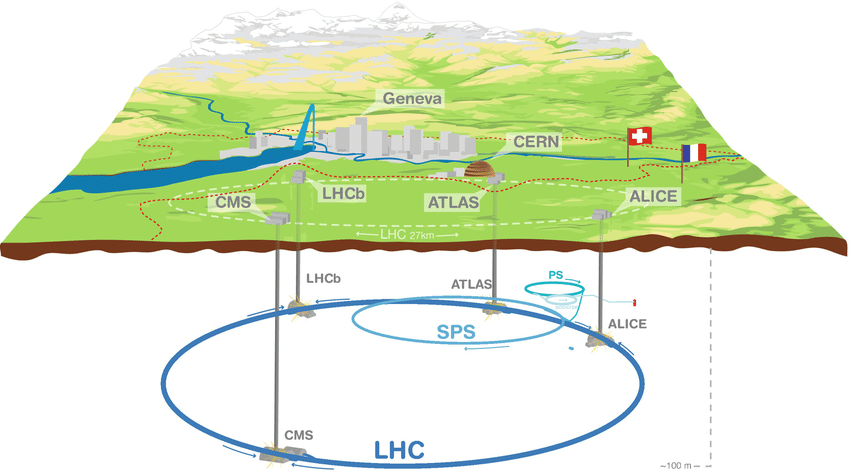
\includegraphics[width = \textwidth]{Chapter2/OverallLHC_1}
 % \caption{Overall view of the LHC including the ATLAS, CMS, ALICE and LHCb experiments. \pablo{This image duplicates the information of Figure~\ref{fig:Chap2:LHC_AcceleratorComplex}}}
%	  \label{fig:Chap2:OverallLHC}
%	\end{figure}

The LHC has two rings with ultra-high vacuum (to prevent collisions with gas molecules 
while moving through the accelerator) in which particle beams travel in opposite directions. 
%The design expected to collide proton beams at a centre-of-mass energy (\CM) up to $14\,$TeV at 
% a luminosity (\lumi) of $10^{34}$\lumiunits (see Section~\ref{sec:Chap2:LHC:lumi} for details about luminosity). 
As well as protons, it can collide heavy ions, in particular lead nuclei. 
% at $\CM=2.3\,$TeV per nucleon and a peak luminosity of \mbox{\lumi$=10^{27}$\lumiunits}~\cite{doi:10.1146/annurev-nucl-102711-094910}.
%These specifications make the LHC the accelerator with higher \CM collision energy~\cite{CERN_LHC_web}. 

The beams in the LHC are made up of bunches of protons that %are spaced $7\,$m apart and 
collide every $25\,$ns. 
Each bunch contains approximately $1.1 \times 10^{11}$  hadrons, being about 2500--2800 the maximum possible 
number of bunches that can be reached with the beam preparation method currently used~\cite{steerenberg2019operation}.
The size of each bunch is approximately $25\,$cm~\cite{Evans_2008}.


% Tunnels
The LHC tunnel lies between $45\,$m and $170\,$m below the surface on a plane inclined at 1.4\% sloping towards the Léman Lake.
The underground construction adds some shielding from outside interferences that could interact with the detectors and cause 
anomalous readings. Even $100\,$m underground, the cosmic rays can reach the detectors, so these are used to help calibrate them.
%The tunnel has an internal diameter of $3.7\,$m, which makes it extremely difficult to install two completely separate proton rings
%\cite{Blewett:103798} as in the Superconducting Super Collider (SSC). Therefore, the counter-rotating rings are built
%under the \textit{two-in-one} twin-bore superconducting magnet design. 
%These twin bore configurations have the disadvantage of having the rings magnetically coupled, which adversely affects flexibility~\cite{Evans_2008}.
%Figure~\ref{fig:Chap2:LHC:DipoleCS} shows an example of the LHC twin-bore dipole magnet.
The two rings are built under the \textit{two-in-one} twin-bore superconducting magnet design~\cite{Evans_2008} .%%&~\cite{Blewett:103798}.

%\begin{figure}
%\centering
%\begin{minipage}{.45\textwidth}
%  \centering
%  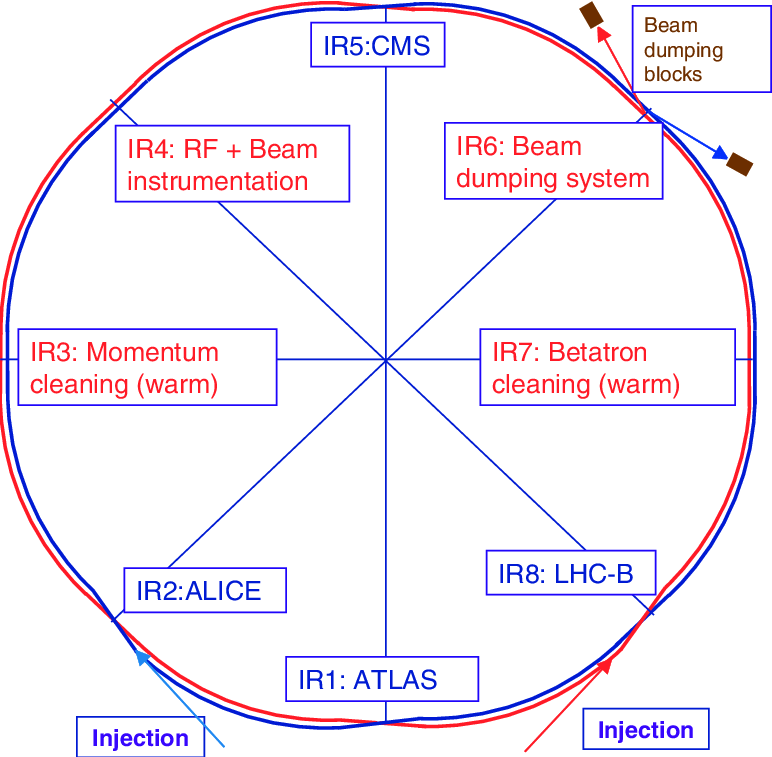
\includegraphics[width=.99\linewidth]{Chapter2/LHC_magnetSystem}
%  \captionof{figure}{Schematic layout of the LHC (Beam 1 clockwise, Beam 2 anticlockwise).}
%  \label{fig:Chap2:LHC:Layaout}
%\end{minipage}%
%\begin{minipage}{.54\textwidth}
%%  \centering
%  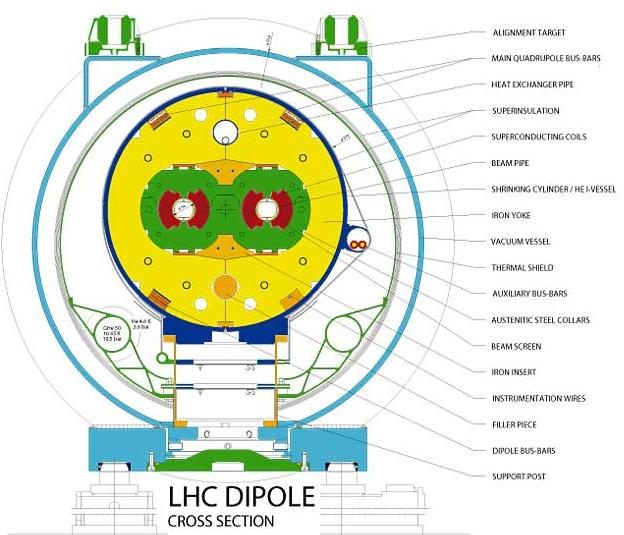
\includegraphics[width=.99\linewidth]{Chapter2/LHC_DipoleCrossSection}
%  \captionof{figure}{LHC dipole cross section.}
%  \label{fig:Chap2:LHC:DipoleCS}
%\end{minipage}
%\end{figure}

% Lattice Layout and Magnet system
%The LHC is not a perfect circle. Approximately $22\,$km of the LHC ring consists of 8 curved sections. 
%The remaining $5\,$km of the tunnel are made of 8 straight sections, denominated insertion regions (IR), that provide space for the experiments.
%Figure~\ref{fig:Chap2:LHC:Layaout} shows the distribution of IR and crossing points for the LHC. This layout follows that
%of the LEP tunnel. The number of crossing points  where the beams pass from one ring to the
%other for colliding was decreased from the original eight at LEP to four in the LHC in order to reduce costs and 
%optimise the utility insertions containing Radio Frequency (RF), the collimation and the
%beam dump systems~\cite{Pettersson:291782}. 

The LHC contains %the dipole bending magnets, which are shown in Figure~\ref{fig:Chap2:LHC:DipoleCS}.The 
1232 twin-bore dipole magnets to curve the trajectory of the particle beams. %that would, otherwise, follow a straight line.
Dipoles are also equipped with additional multipole-lattice magnets (sextupole, octupole and decapole), which correct for small imperfections 
in the magnetic field at the extremities of the dipoles. 

%Each of the eight straight sections is approximately $528\,$m long. The RF cavities delivering
%$2\,$MV (an accelerating field of $5\,$MV/m) at $400\,$MHz are located in the IR4. 
%The 16 RF cavities compensate the synchrotron radiation
%losses (the electromagnetic radiation emitted when charged particles travel in curved paths) that
%take place at the arcs of LHC.
%Since the protons loose much less energy than electrons in a circular collider\footnote{The
%energy radiated per particle by synchrotron radiation is proportional to the 
%inverse of the mass of the particle: $\Delta E \propto 1/m^4$. }, the LHC would have
%profited from more circular sections. However, re-using LEP tunnels was preferred in terms of cost.
%During the 20 minutes that are needed to reach the beams maximum energy,
%the bunches have passed the RF cavities more than 10 million times~\cite{Pettersson:291782}.

The Radio Frequency (RF) cavities (also known as resonators) %are metallic chambers spaced at intervals along the accelerator shaped to resonate at 
%specific frequencies, 
allow radio waves to interact with passing particle bunches. The main role of
the RF cavities is to keep the proton bunches tightly packed to ensure the required luminosity at
the interaction point (IP). They also transfer RF power to the beam to accelerate it to the target energy.

At the insertion of the arc and straight sections, quadrupole magnets are installed to suppress
the dispersion of particles. Acting as focal lenses, quadrupole magnets gather the particles 
together.  %This system not only cancels the horizontal dispersion arising in the arc but also
%adapts the LHC reference orbit to the geometry of the LEP tunnel. 
%Before entering the detectors, the inner triplets (which are made mostly from quadrupoles)
%tighten the beam, from $0.2\times 10^{-3}\,$m  down to $16\times 10^{-6}\,$m. These are known as insertion magnets.

In total, there are more than 9000 magnets all over the LHC and more than 50 types of magnets are needed to
 make the particles circulate in their path without losing speed.
The coils are made of niobium-titanium (NbTi)  which is cooled to less than $2\,$K with superfluid helium to reach superconductivity. 

\begin{comment}
Of course, only stable charge particles\footnote{Long-lived particles such as the muon ($\tau \approx 2\times10^{-6}$ s) are discussed to be 
used on a muon collider~\cite{Long:2020wfp}.} such as electrons, positrons, protons, antiprotons and some ions, can be accelerated by
the magnetic fields described. The force that experiments a charged particle with charge $q$ moving under a magnetic field $B$ at
a speed $v$ is given by Lorentz law
\begin{equation}
	\overrightarrow{F} = q \overrightarrow{v} \times \overrightarrow{B}
\end{equation}
and, since $\overrightarrow{B}$ is perpendicular to $\overrightarrow{v}$, this force is always directed to the centre of the circle of radius $r$:  $F = Bqv = m\frac{v^2}{r}$.
\end{comment}


%A proton machine such as LHC does not have the same synchrotron
%radiation problem and would, ideally, have longer arcs and shorter straight sections for the same
%circumference, but accepting the tunnel “as built” was the cost-effective solution. However, it was
%decided to equip only four of the possible eight interaction regions and to suppress beam crossings
%in the other four to prevent unnecessary disruption of the beams.

%&&&%%%%%%%%%%%%%%%%%%%
%      	LHC - Accelerator Complex         %
%%%&&&%%%%%%%%%%%%%	%%%%
\subsection{Accelerator complex}
\label{sec:Chap2:LHC:AcceleratorComplex}
To accelerate the proton beams, the existing CERN accelerator complex is used.
These accelerators were, back in the day, the state of the art colliders and now they serve
as injection system for the LHC. The path followed by the particle beams is presented in
 Figure~\ref{fig:Chap2:LHC_AcceleratorComplex}. The accelerator complex consists of
several machines interconnected to boost the beams until these reach the LHC.

The proton bunches are produced by ionising a gas of hydrogen atoms and then they are accelerated to a
momentum of 50 MeV by the linear accelerator (LINAC2). %Starting from Run 3, the LINAC2 is being replaced by
%the LINAC4. 
After being produced, the beams enter the first circular accelerator, the Proton Synchrotron 
Booster (PSB), which has 630 m radius and increases the energy of the protons up to 1.4 GeV.
Right after the PSB, the PS brings the particles up to $25\,$GeV. 
It is followed by the SPS, which raises the energy of the particles to 450 GeV. % SPS = 6.9 km  
%Once the protons have 450 GeV, the minimum energy at which the LHC can maintain a stable beam, they
Then, the beam is injected into the LHC by two different  transfer injection (TI) lines~\cite{Lari:1069714}. % $2\,$km long transfer injection lines
%Protons will circulate in the LHC for 20 minutes until reaching the nominal beam energy~\cite{Evans_2008}.
 
Heavy-ion collisions were included in the conceptual design of the LHC from an early stage and 
follow the same path to maximum acceleration as the protons. Lead ions are extracted from a source 
of vaporised lead and are initially accelerated by the Low Energy Ion Ring (LEIR). 

	
	\begin{figure}
 	  \centering
 	  \includegraphics[width = \textwidth]{Chapter2/CCC-v2022}
	  \caption{Scheme of CERN accelerator complex.}
	  %Protons are injected from the LINAC2 into the PS Booster, then the PS, 
	  %followed by the SPS, before finally reaching the LHC.}
	  \label{fig:Chap2:LHC_AcceleratorComplex}
	\end{figure}

%&&&%%%%%%%%%%%%%%%
%      	LHC - Experiments       %
%%%&&&%%%%%%%%%%%%%	
\subsection{LHC experiments}
%In the LHC are carried 4 major experiments: ATLAS, CMS, LHCb and ALICE. The detectors for these experiments
%are shown in Figure~\ref{fig7:Chap2:LHC_experiments}.
%In the 4 interaction points of LHC (described in Figure~\ref{fig:Chap2:LHC:Layaout}) are located the four detectors. 
%The IR1 and IR5 house the high luminosity experiments of the LHC: ATLAS and CMS respectively. These IR 
%are identical in terms of hardware and optics being the only difference that the crossing-angle is in the vertical plane
%in Point 1 and in the horizontal plane in Point 5~\cite{Evans_2008}. 
%The straight sections of IR2 and IR8, with medium luminosity, host the ion experiment ALICE and LHCb detector.
%Luminosity levelling is usually applied for the two low luminosity experiments in IP2 and IP8.


In the LHC four major experiments are carried out, each of them with its own detector (see Figure~\ref{fig7:Chap2:LHC_experiments})
and physics programme.
%These particle detectors measure particles produced as debris from the $\Pproton \Pproton$ (or lead) collisions through the interaction
%with the material of the sub-detectors. 
Distributed along the collider as is shown in Figures \ref{fig:Chap2:LHC_AcceleratorComplex}, 
these highly sophisticated experiments are:
\begin{itemize}
  \item \textbf{A Toroidal LHC ApparatuS (ATLAS)}~\cite{ATLAS:2008xda}:
  		It is a generic multi-purpose experiment for high luminosity. %(up to \lumi = $10^{34}$\lumiunits)
		It studies $\Pproton \Pproton$ collisions and investigates a wide range of physics, from the SM to the search for extra dimensions or
		dark matter. It has the dimensions of a cylinder, $46\,$m long, $25\,$m in diameter. The ATLAS detector weighs $7\times 10^{3}$ tonnes.
		%Similar to the weight of the Eiffel Tower
		Its design features excellent jet and missing transverse energy resolution, particle identification and flavour tagging
		and standalone muon measurements.  %A scheme of this detector is shown in Figure~\ref{fig7:Chap2:LHC_experiments:ATLAS}.
		ATLAS is covered in detail in Section~\ref{sec:Chap2:ATLAS} as it is the detector used to perform the analysis presented in
		this thesis.
	
  \item \textbf{Compact Muon Solenoid (CMS)}~\cite{CMS:2008xjf}: 
  		It is the other general-purpose experiment for high luminosity. %(same \lumi  as ATLAS). 
		CMS has the same objectives and goals as ATLAS but both its hardware and software designs are different. 
		Even though CMS is smaller than ATLAS ($21\,$m long, $15\,$m in diameter) it is much heavier, weighting  $14\times 10^{3}$ tonnes.
		The bulk of its weight is the steel yoke that confines the $4\,$T magnetic field of its superconducting solenoid.
		%At the core of the CMS detector sits a high-magnetic-field and large-bore superconducting solenoid surrounding 
		%an all-silicon pixel and strip tracker, a lead-tungstate scintillating-crystals electromagnetic calorimeter, and a brass-scintillator 
		%sampling hadron calorimeter
		The design of CMS emphasises magnificent electron/photon energy and momentum resolution. 
		%Figure~\ref{fig7:Chap2:LHC_experiments:CMS} illustrates this device. 
		The role of the coexistence of CMS and ATLAS is fundamental so that the scientific community 
		can verify and confirm the independent results found by these experiments.
		
		
  \item \textbf{Large Hadron Collider beauty (LHCb)}~\cite{LHCb:2008vvz}:
    		It is a lower luminosity\footnote{By lower luminosity it means that less collisions are delivered by the LHC the experiment.}
		 experiment designed to study the small asymmetries between matter and antimatter through \CP violation using rare decays
		of \Pbottom-quark based hadrons. 
		The detector is arranged as a succession of planar sub-detectors %(as can be seen in Figure~\ref{fig7:Chap2:LHC_experiments:LHCb})
		since most of the \Pbottom-flavoured mesons follow the beam-pipe direction
		when created in the $\Pproton \Pproton$ collision. LHCb delivers remarkable low-momentum track reconstruction and particle identification. 

  \item \textbf{A Large Ion Collider Experiment (ALICE)}~\cite{ALICE_Collaboration_2008}:
  		It is a low luminosity experiment in IR8 that focuses on QCD. %, the strong-interaction sector of the SM. 
		The main feature of ALICE is a  general-purpose detector that uses heavy-ion collisions to 
		 study matter interacting at extreme densities and temperatures, thus reproducing the quark-gluon plasma.
		 This detector provides highly efficient 
		 track reconstruction in an environment full of heavy ions.
		 Besides running with lead ions, the physics programme includes collisions with lighter ions, 
		 lower energy collisions and a dedicated proton--nucleus run.

\end{itemize}


\begin{figure}[ht] 
  \begin{subfigure}[b]{0.5\linewidth}
    \centering
    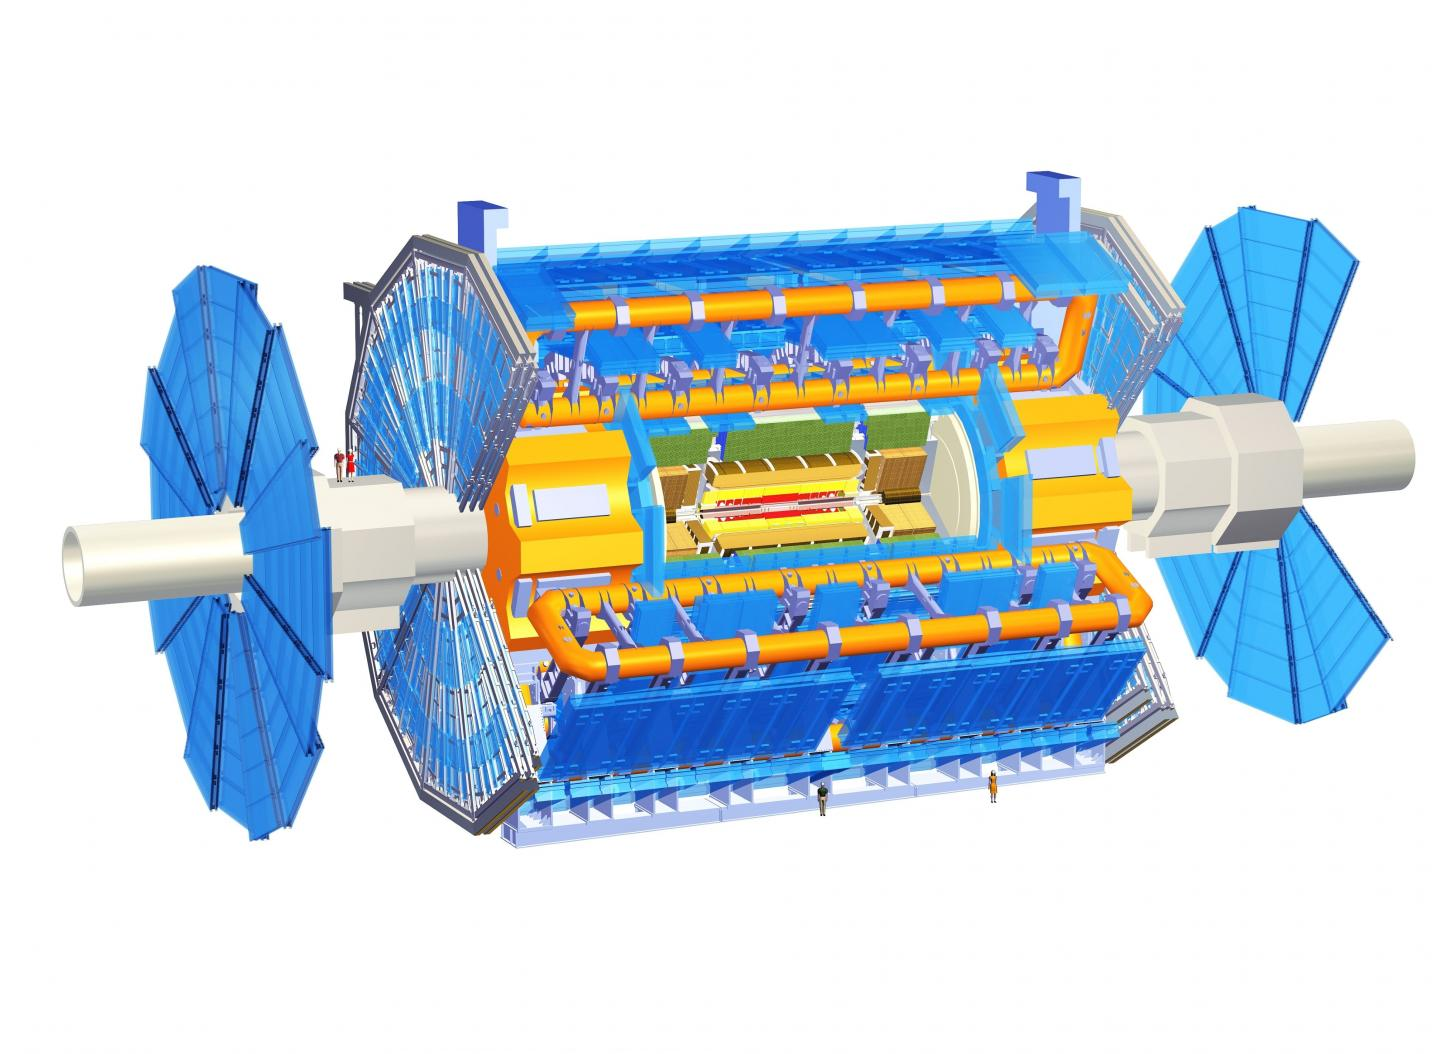
\includegraphics[width=.99\linewidth]{Chapter2/Experiments_ATLAS} 
    \caption{ATLAS} 
    \label{fig7:Chap2:LHC_experiments:ATLAS} 
    \vspace{4ex}
  \end{subfigure}%% 
  \begin{subfigure}[b]{0.5\linewidth}
    \centering
   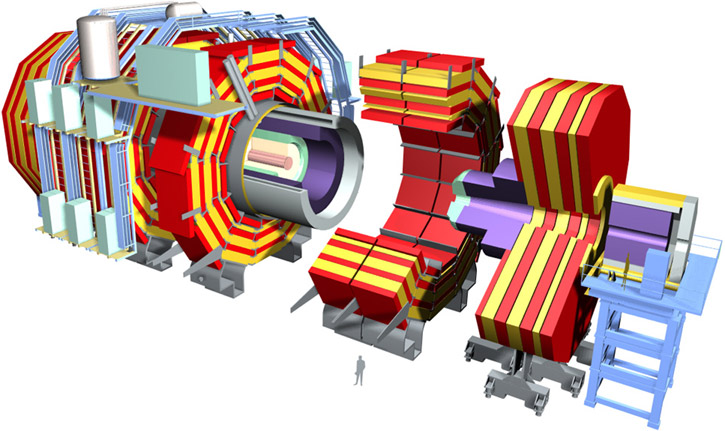
\includegraphics[width=.99\linewidth]{Chapter2/Experiments_CMS}
    \caption{CMS} 
    \label{fig7:Chap2:LHC_experiments:CMS} 
    \vspace{4ex}
  \end{subfigure} 
  \begin{subfigure}[b]{0.5\linewidth}
    \centering
    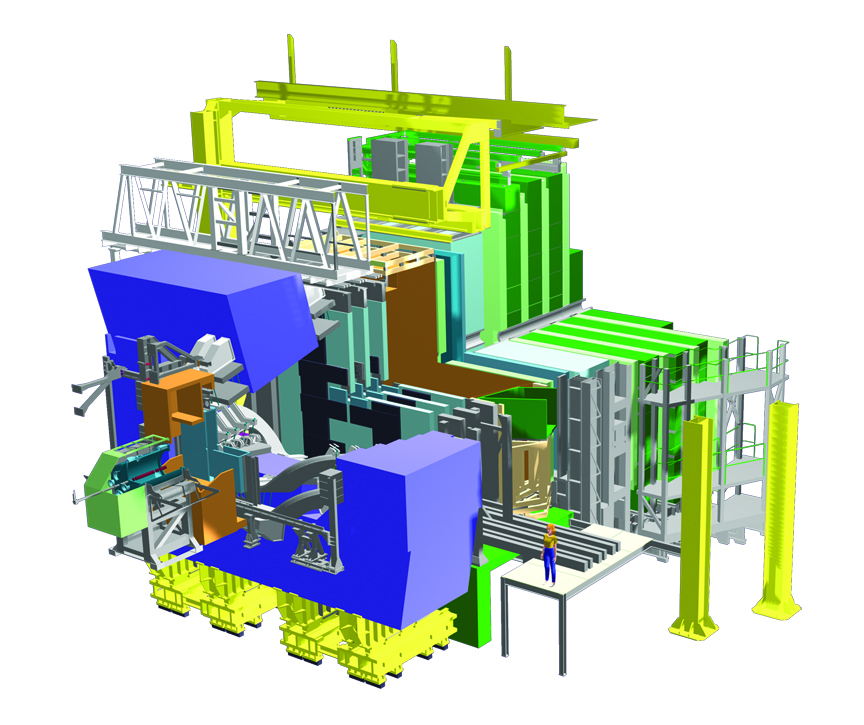
\includegraphics[width=.9\linewidth]{Chapter2/Experiments_LHCb_lowres}
    \caption{LHCb} 
    \label{fig7:Chap2:LHC_experiments:LHCb} 
  \end{subfigure}%%
  \begin{subfigure}[b]{0.5\linewidth}
    \centering
    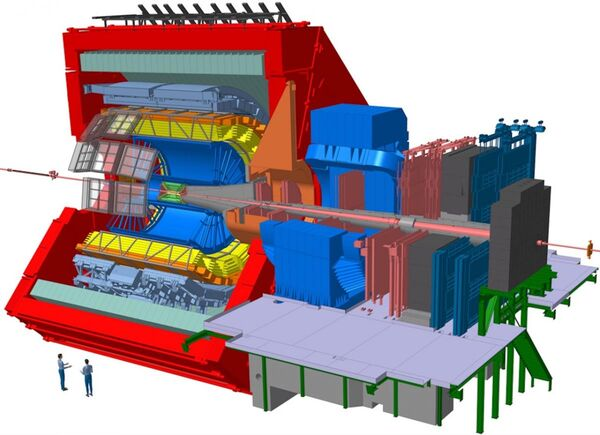
\includegraphics[width=.9\linewidth]{Chapter2/Experiments_ALICE}
    \caption{ALICE} 
    \label{fig7:Chap2:LHC_experiments:ALICE} 
  \end{subfigure} 
  \caption{Scheme of LHC main experiments. Note that the images are not equally scaled.}
  \label{fig7:Chap2:LHC_experiments} 
\end{figure}

Along the LHC machine, there are other experiments much smaller than ATLAS, CMS, LHCb and ALICE, typically sharing the cavern with the major projects. 
The most relevant among the minor experiments are LHCf~\cite{LHCf:2008lfy}, MATHUSLA~\cite{MATHUSLA:2018bqv}, MilliQan~\cite{Yoo:2645863}, 
MoEDAL~\cite{Mitsou:2017doz}, TOTEM~\cite{Collaboration_totem_2008} and FASER~\cite{FASER:2018ceo}.
 
\begin{comment}
\begin{itemize}
  \item \textbf{The Large Hadron Collider forward (LHCf)}~\cite{LHCf:2008lfy}: Uses particles thrown forward by collisions in the Large Hadron 
  			Collider as a source to simulate cosmic rays in laboratory conditions. It shares its cavern with the ATLAS detector~\cite{Adriani:926196}.
  \item  \textbf{The Massive Timing Hodoscope for Ultra Stable neutraL pArticles (MATHUSLA)}~\cite{MATHUSLA:2018bqv}: Is dedicated large-volume 
  			displaced vertex detector for the HL-LHC on the surface above ATLAS or CMS for the search for neutral long-lived particles.
  \item  \textbf{MilliQan}~\cite{Yoo:2645863, PhysRevD.102.032002}: Consists on a small-scale detector experiment aiming to detect millicharged particles, i.e., particles with charges 
  			much smaller than that of the electron.
  \item \textbf{Monopole and exotic particle detector at the LHC (MoEDAL)}~\cite{Mitsou:2017doz}: Deployed at LHCb cavern, it is optimised to detect 
  			highly ionising particles such as magnetic monopoles, dyons and multiple-electrically charged stable massive particles predicted in a number 
			of theoretical scenarios. %Recent Result: https://webific.ific.uv.es/web/content/el-experimento-moedal-publica-nuevos-resultados-para-encontrar-una-de-las-part%C3%ADculas-m%C3%A1s?fbclid=IwAR20NTNBJyzMktkraC4c6ixcxwYdGgm_ygIt1VcmRg562FUDASzm5H0TWT8
  \item \textbf{TOTEM}~\cite{Collaboration_totem_2008}:  Aims to measure the total cross-section of $\Pproton \Pproton$ interaction using a luminosity-independent method 
  			and study elastic and diffractive scattering at the LHC. As CERN longest experiment, TOTEM detectors are spread across almost half a kilometre 
			around the CMS IP.
  \item \textbf{ForwArd Search ExpeRiment (FASER)} ~\cite{FASER:2018bac, FASER:2018ceo}: Designed to search for new, yet undiscovered, light and 
  			weakly-interacting particles and study the interactions of high-energy neutrinos.
\end{itemize}
\end{comment}

%&&&%%%%%%%%%%%%%
%         	LHC - Grid	       %
%%%&&&%%%%%%%%%%%
\subsection{LHC computing grid}
\label{sec:Chap2:LHC:LCG}
The data collected by the different LHC experiments is stored, processed and, then, 
made available for all the researchers of each collaboration. %\footnote{Within the grid context, 
%each collaboration is known as Virtual Organisation (VO).}.
This is possible thanks to the last piece of the LHC, its computing model and infrastructure: the World LHC Computing Grid (WLCG). It consists
of several computing farms distributed around the world and interconnected. 
%Figure~\ref{fig:Chap2:LHC_Grid} shows the geographical distribution of the different facilities that comprise the LCG.
%Just as the WWW enables access to information, the Grid enables access to computer resources. Employing a grid certificate, is possible for any user to run jobs
%on the grid and to access the data stored. The implementation of the grid model implies an effective coordination among all LHC collaboration centres~\cite{Bird:2005js}. 

%	\begin{figure}
% 	  \centering
% 	  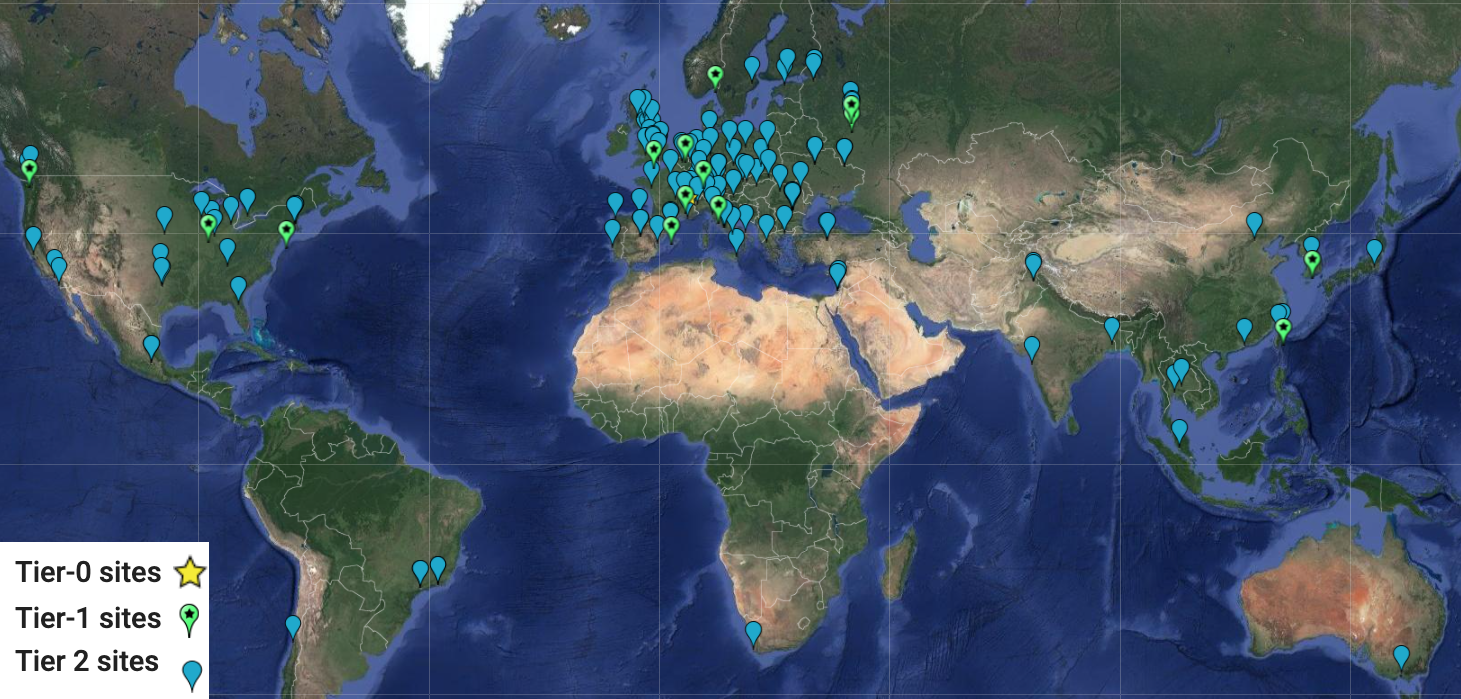
\includegraphics[width = \textwidth]{Chapter2/WorldWideGrid_1}
%	  \caption{Worldwide LHC Computing Grid geolocalisation of sites~\cite{CERN_LHCG_locations}.}
%	  \label{fig:Chap2:LHC_Grid}
%	\end{figure}

Different types of computing centres are defined and these are classified into Tiers~\cite{Duckeck:2005rb}:
\begin{itemize}
	\item \textbf{Tier-0}: Facility located at CERN and responsible for providing  prompt reconstruction 
				       and distributing a copy of the raw data to the Tier-1 centres.
				%This facility is located at CERN and it is responsible for archiving (first copy) and distributing the raw data received from the Event Filter, i.e., 
				%the data emerging from the Data Acquisition systems (DAQ) after the trigger.
				%It provides prompt reconstruction and distributes a copy of the raw data to the Tier-1 centres.
				%	RAW	:	Raw data				-->   Events as output by the Event Filter
				% Derived datasets: ESD, primary AOD and TAG set.
				%	ESD :	 Event Summary Data  	-->  Event data written as the output of the reconstruction process
				%     AOD	:	 Analysis Object Data	-->  A reduced event representation, derived from ESD, suitable for analysis
				%.    TAG	: 	 Tag Data		      		-->  Event-level metadata  to support efficient identification and selection of events of interest to a given analysis
	\item \textbf{Tier-1}: Facilities archiving the raw data permanently and providing the computational capacity for reprocessing and physical
				analysis. These also store the simulated and reprocessed data.  Currently, 13 computer centres are serving as Tier-1,  %(see Figure~\ref{fig:Chap2:LHC_GridTier}).
				making data available to the Tier-2 centres~\cite{CERN_LHCG_centres}.
				% modest RAW and ESD
	\item \textbf{Tier-2}:  Facilities typically located at universities and scientific institutes, that serve
					as storage and analysis facilities of processed data. The event simulations
					are also executed here. 
				%there are more than 150 Tier-2 sites. The derived datasets produced by the physics groups 
				%are copied to the Tier-2 facilities for further analysis. The MC simulations for event production are executed at this level.
	\item \textbf{Tier-3}: Local computing resources. %from local clusters to even just an individual PC are referred to as Tier-3. There is no formal 
				%engagement between worldwide LCG and the Tier-3.
\end{itemize}
%	\begin{figure}
% 	  \centering
% 	  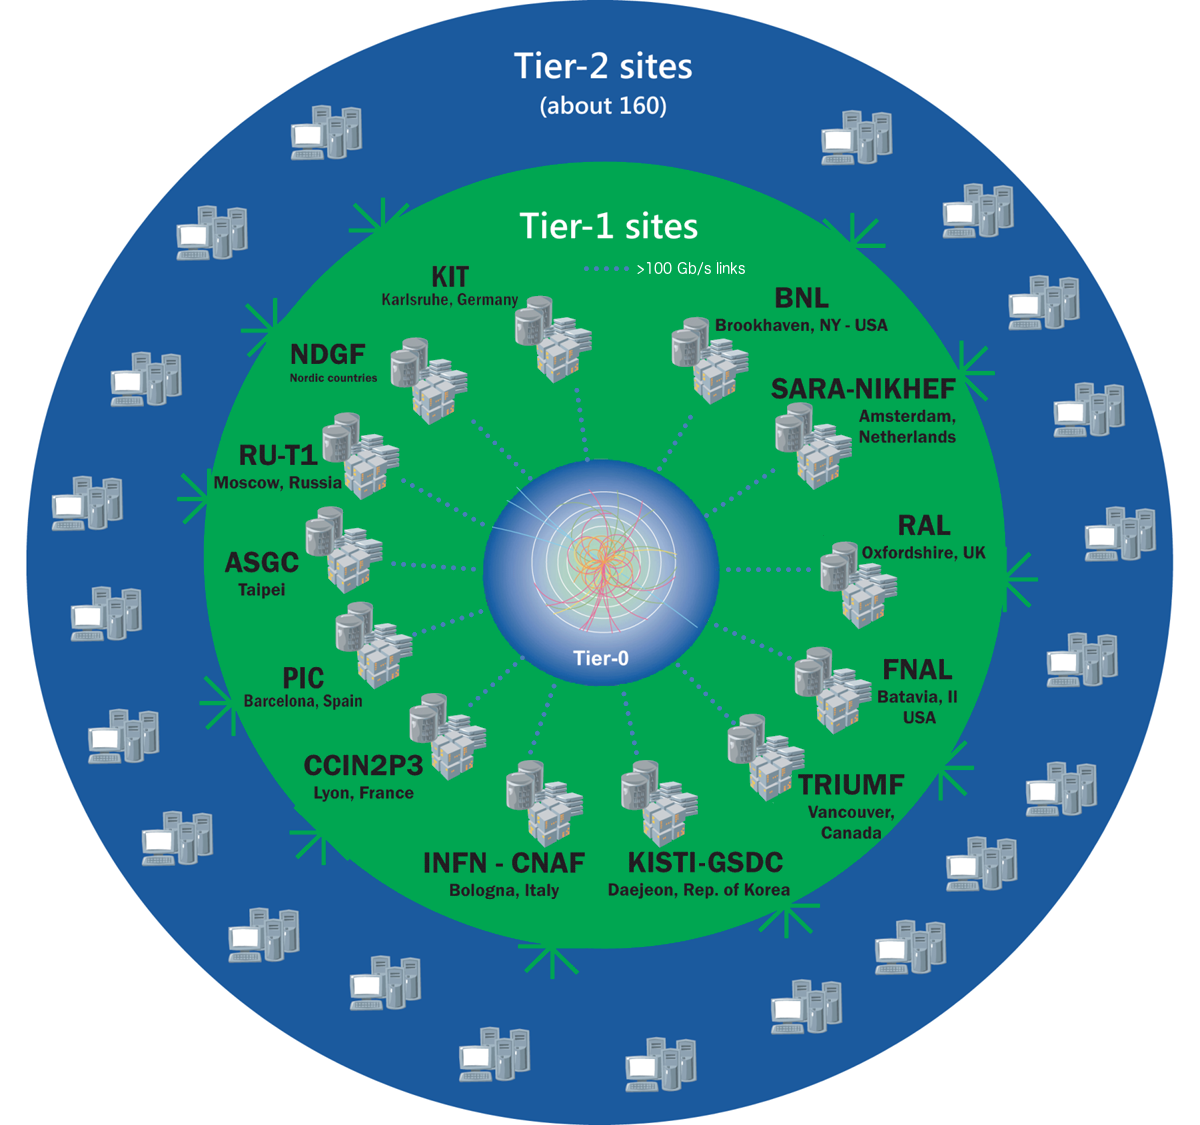
\includegraphics[width = 0.7\textwidth]{Chapter2/GridTiers}
%	  \caption{Distribution by Tiers of the LCG~\cite{CERN_LHCG_centres}. This project provides global computing resources to store, 
%	  distribute and analyse  the data recorded at the LHC.}
%	  \label{fig:Chap2:LHC_GridTier}
%\end{figure}

This system provides near real-time access to LHC data worldwide. %The LCG collaboration spreads out over 42 countries with 170 computing centres and 1 million computer cores, being the world's largest computer grid. 
It deals with  over two million tasks daily. These specifications make the LCG the most sophisticated system for data taking and analysis ever built for science.






%%%%%%%%%%%
%           ATLAS        %
%%%%%%%%%%%
\section{The ATLAS detector}
\label{sec:Chap2:ATLAS}


%Installed in its experimental cavern at point 1, 
The ATLAS detector is the largest detector ever constructed for a particle collider. 
It is designed to record events of high-energy colliding particles at high luminosities.
The thousands of millions of interactions that take place at the centre of the ATLAS detector are recorded and processed by the
different sub-detectors, which are composed of more than 100 million electronic channels. Each ATLAS sub-detector
is sensitive to a different type of particle and to different properties. Therefore, the layered structure allows for effective particle identification, as well as  
enables accurate measurements of energy and momentum. Figure~\ref{fig:Chap2:ATLAS:GeneralOverview} shows an overall layout of the ATLAS 
detector and identifies its different sub-detectors. In the picture, one can appreciate that the cylindrical shape of ATLAS is divided into two parts: the ``barrel'' 
and the two ``end-caps''. In the barrel region, the sub-detectors are built as coaxial layers around the beam pipe. %(see meme \ref{fig:Chap2:ATLAS:Shrek}).
As one moves away from the axis, it finds the Inner Detector (ID), the solenoid magnet, the Electromagnetic (ECAL) and Hadronic (HCAL) calorimeters, and
the Muon Spectrometer (MS) and the toroid magnet in the outermost layers. 
The technical details of these sub-detectors and the magnet systems are presented in Sections\,\ref{sec:Chap2:ID}, 
\ref{sec:Chap2:CALO}, \ref{sec:Chap2:ATLAS:MS} and \ref{sec:Chap2:MagnetSystem}.

\begin{figure}
	\centering
 	 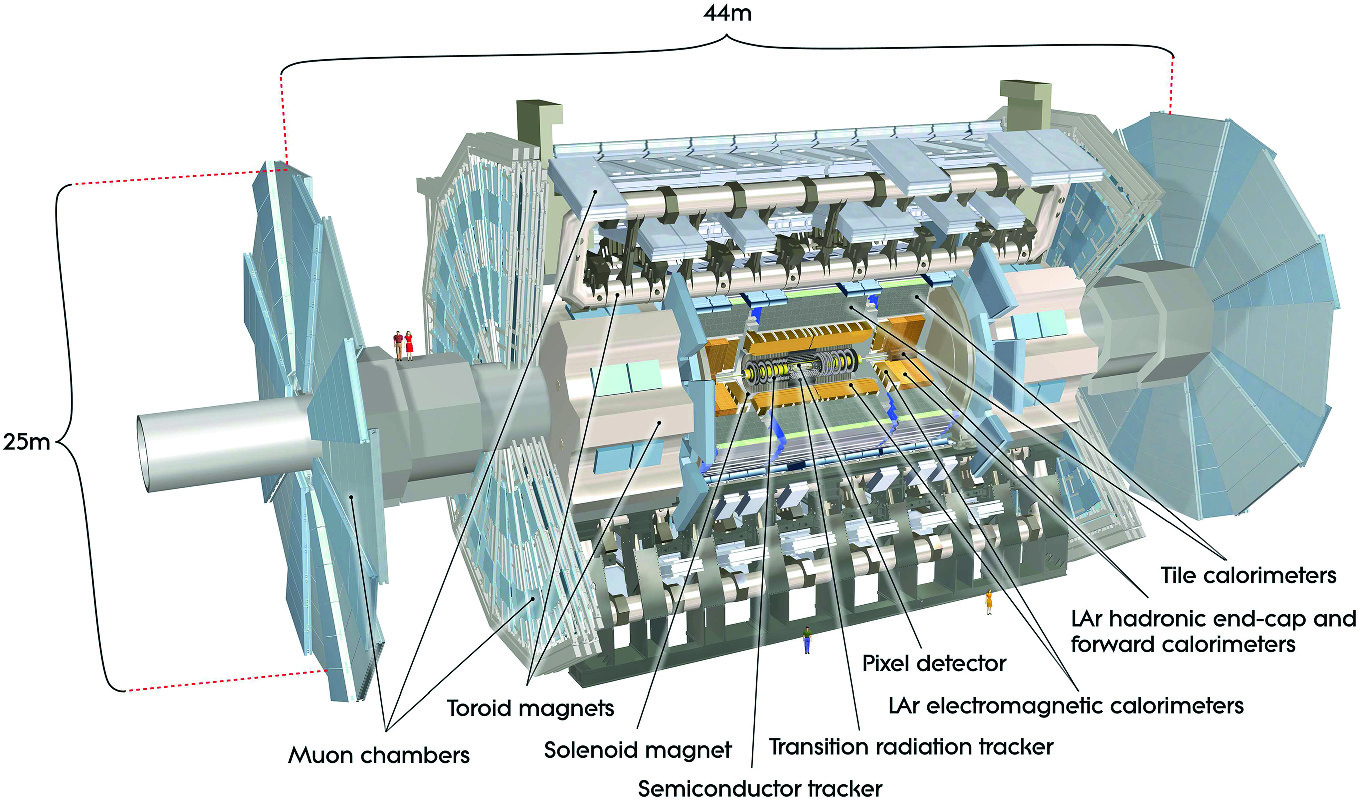
\includegraphics[width = \textwidth]{Chapter2/ATLAS_Subdetectors}
	 \caption{Simulated schematic view of the ATLAS detector~\cite{Pequenao:1095924}.}
	\label{fig:Chap2:ATLAS:GeneralOverview}
\end{figure}

%\begin{figure}
%	\centering
% 	 
\includegraphics[width = 0.7\textwidth]{Chapter2/Shrek}
%	 \caption{Due to its coaxial-layered structure ATLAS can be understood 
%	as cylindric onion: ``\textit{ATLAS have layers, onions have layers}''~\cite{Shreck}.}
%	\label{fig:Chap2:ATLAS:Shrek}
%\end{figure}


 The ATLAS detector can explore a wide range of phenomena with high precision.
 It was designed to perform precision measurements of the SM parameters and the Higgs
 boson properties.
 
  %This is why, since the mass of the Higgs boson was not known at that time, its performance 
  %requirements cover a large mass range for
  %the Higgs decay products.

 
 \begin{comment}
 The stone for the foundations of ATLAS was laid in March 1992 at the critical ‘Towards the LHC Experimental Programme’ 
 meeting, where physicists proposed several possible experiments for the LHC~\cite{LHC_fundations}. Two  %~\cite{LHC_CernCouncil_Experiments}
 projects based on large toroidal magnet systems were proposed EAGLE and ASCOT. %~\cite{Norton:1076511}.
  By the summer of that year, both experiments merged into ATLAS. In October 1992, the letter of intent of the ATLAS
 Collaboration was sent to the LHC Experiments committee and, in 1994, the technical proposal~\cite{ATLAS_TechnicalProposal}.
 In 1997 the formal approval of the ATLAS experiment arrived and one year later the excavation on the cavern began.
 The cavern was inaugurated five years later and the construction of the ATLAS detector ended in 2008.  Later, in 2009, at
 $\CM = 2.36\,$TeV, ATLAS records its first collisions~\cite{collaboration:1228300}. 
\end{comment}
 
 %One of the most important milestones for ATLAS (and for all science in the last decades) was the observation of a particle %(see \ref{sec:Chap1:HiggsPhys_discovery})
 %consistent with the Higgs boson in July 2012.  In 2016,  the combination of
 %ATLAS and CMS measurements for Higgs-boson production on decay rates with Run 1 data was published~\cite{ATLAS:2016neq}.
 %After that, the physics programme at $13\,$TeV allowed precision studies of the Higgs boson and other SM particles, as well as the 
 %search for new particles with other masses. 
 
 %As already described in Section~\ref{sec:Chap1:HiggsPhys_discovery}, the Higgs boson was discovered on 2012.
 %This is the most important milestones for ATLAS (and for all science in the last decades).
 %Other relevant items in ATLAS timeline are the observation and rate measurement of \ttbar events~\cite{ATLAS:2010zaw} or
 %the evidence for rare electroweak $\PWpm\PWpm$ production~\cite{ATLAS:2014jzl}. The first evidence of light-by-light scattering 
 %at high energy was also found with ATLAS~\cite{ATLAS:2017fur}. The first \ttH associate production~\cite{ATLAS:2017fak} and 
 %$\PHiggs \rightarrow \Pbottom \APbottom$ decays~\cite{ATLAS:2018kot} were observed for first time by ATLAS too.
%  \pablo{También podría dedicar una linea al technology transfer \url{https://atlas.cern/discover/detector/technology-transfer}}

%\subsection{Objective and physics programme}
%\pablo{Esto queda comentado en la introducción a ATLAS pero podría moverlo a esta sección y extenderlo / reestructurarlo}
%More about ATLAS scientific programme \url{https://inspirehep.net/files/315b42523bf67133e14db36eb9946109}

 % ATLAS GOALS: 
 % - Precision measurements of the properties of the Higgs Boson: Couplings to fermions, Couplings to W/Z, diff. cross-sections, Self-coupling, Scalar Higgs boson vs. BSM composite
 % - Precision SM Measurements: Forward/backward asymmetry, Vector-boson scattering, Precision top mass and cross-sections
 % - Searches for BSM Signatures: Long-lived particles, New resonances, SUSY, SUSY top partners, Dark matter, Searches for new vector bosons
 % - Flavour Physics: Lepton Flavour Violation, Searches for FCNC in top decays, Rare B-meson decays
 % - Heavy-Ion Physics: Light-by-light scattering, Electroweak production, In-medium parton energy loss (jets in PbPb), Quarkonia production
 %The physics programme of ATLAS is driven by the following topics~\cite{CERN-LHCC-2017-020}:
 %\begin{itemize}
 %	\item Precision measurements of the Higgs-boson properties: This includes the couplings of the Higgs to the SM fermions, area in
 %		which the work developed at this thesis is contextualised. Other subjects are the couplings to \PW and \PZ, 
 %		differential cross-sections, self coupling, etc.
 %		
 %	\item Precision SM Measurements: Such as precision top mass and cross-sections, vector-boson scattering and forward/backward asymmetry.
 %
 %	\item Searches for BSM Signatures: New resonances. SUSY,  dark matter, extra dimensions, searches for new vector bosons and long-lived particles.
 %
 %	\item Flavour Physics: This field includes the searches for FCNC in top decays, rare $B$-meson decays and lepton flavour violation.
 %
 %	\item Heavy-Ion Physics: The Pb-Pb physics programme focusses on in-medium parton energy loss, 
 %		electroweak and quarkonia production, and light-by-light scattering.
 %
  %\end{itemize} 
%Topics: precise measurements of the SM~\cite{Amoroso:2709980}, super-symmetry studies~\cite{Pacey:2789157},
 %sources of \CP-violation~\cite{PhysRevD.103.055008}, large \MET dark-matter searches~\cite{Carlson:2727868}, astroparticle physics~\cite{Pinfold:2008zza}, 
 %extra dimensions~\cite{ATLAS:2009sdo} and others. 
 
 
 % ATLAS SM:
 %.      - Higgs: https://inspirehep.net/files/6c0b1f30a286a7aca715341b4fd90442
 % ATLAS SUSY: https://twiki.cern.ch/twiki/bin/view/AtlasPublic/SupersymmetryPublicResults
%The ATLAS project is not only a detector but also a collaboration of people composed of 
%more that 5000 members including physicists, engineers, technicians, doctoral students 
%and support staff. Working at CERN or at any of the 181 institutions that constitute ATLAS,
%the different teams work collaboratively to achieve success.  % Any output by any of the teams 
% comprising ATLAS is shared with the rest of the collaboration and subjected to a strict review 
% process before making the results public, ensuring high-quality standards.
 
 


%%%%%%%%%%%%%%%
%        Coordinate system    %
%%%%%%%%%%%%%%%
\subsection{Coordinate system}
\label{sec:Chap2:ATLAS:CoordinateSystem}
The ATLAS detector uses a right-handed system with its origin at the IP where the collisions take place. 
On one side, there are the (\textit{x, y, z}) cartesian coordinates. The \textit{x}-axis is pointing towards the centre of the ring 
circumference, the \textit{y}-axis is perpendicular to the plane defined by the LHC ring and it points to the surface, and the \textit{z}-axis
is defined by the direction of the beam. 
On the other side, it is more frequent to employ the cylindrical coordinates $(r, \phi, z)$ or the system defined by the azimuthal angle ($\phi$)
and the pseudorapidity, being $\eta = -\textrm{ln}\left[ \textrm{tan}(\theta/2)\right]$
%
%\begin{minipage}{.45\textwidth}
%\begin{align*}
%	\eta &= -\textrm{ln}  \left[ \textrm{tan} \left( \frac{\theta}{2}\right) \right]
%\end{align*}
%\end{minipage}
%\begin{minipage}{.45\textwidth}
%  \centering
% 	 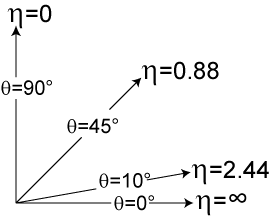
\includegraphics[width = 0.7\textwidth]{Chapter2/Pseudorapidity2}
%\end{minipage}
%
where $\theta$ is the polar angle\footnote{Defined as the angle between the particle three-momentum, $\overrightarrow{p}$ and the positive direction of the beam axis.}.  
%As the polar angle approaches zero, pseudorapidity tends towards infinity.
The change in pseudorapidity $\Delta \eta$ is Lorentz invariant under boosts along the beam axis.
%The use of $\eta$ is preferred over $\theta$ because the distribution of events typically looks flat with respect to $\eta$.
%In terms of the momentum, the above equation can be expressed as:
%\begin{equation*}
%	\eta = -\textrm{ln} \left( \frac{|\overrightarrow{p}| + p_z}{|\overrightarrow{p}| - p_z}\right) 
%\end{equation*}
%being $p_z$ the momentum along the beam direction.
%The rapidity ($y$) is used when dealing with massive particles and it can be expressed 
%as $y = \frac{1}{2}log[(E+p_{z})/(E-p_{z})]$, being $E$ the energy of the particle.
%the energy projection of the momentum in the \textit{z}-axis. 
%Note that when the particles approach the speed of light, 
%they are in the limit $E \approx |\overrightarrow{p}|$ and the values for rapidity and 
%pseudorapidity converge.
The angular distance is measured in units of $\dR = \sqrt{(\Delta \eta)^{2}+(\Delta \phi)^{2}}$, which is invariant under a boost along the 
\textit{z}-axis.  %\footnote{The $\Delta R$ is measured between to vectors, therefore, $\Delta \eta = \eta_2 - \eta_1$ and $\Delta \phi = \phi_2 - \phi_1$.}.
 Figure~\ref{fig:Chap2:ATLAS:CoordinateSystem} shows the coordinate system of ATLAS for both cartesian and cylindrical coordinates. 

\begin{figure}
	\centering
 	 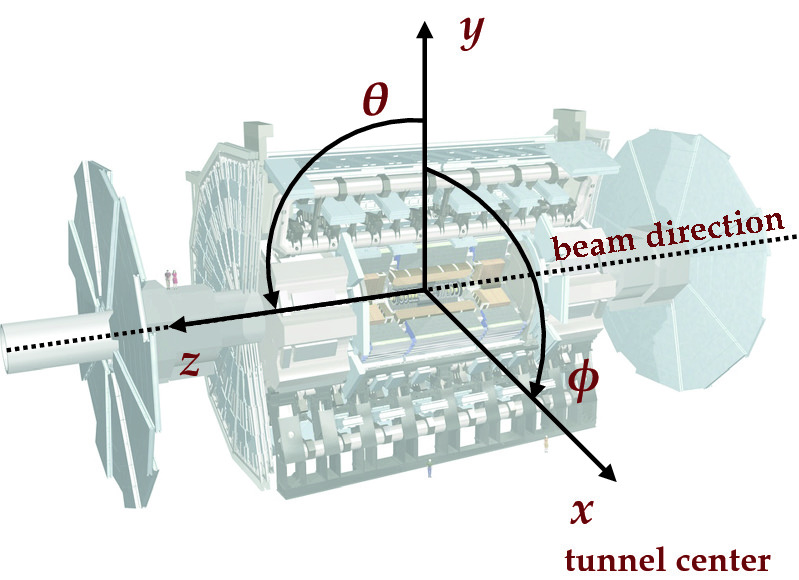
\includegraphics[width = 0.75\textwidth]{Chapter2/ATLAS_CoordinateSystem}
	 \caption{Coordinate system of the ATLAS detector in the context of LHC.}
	\label{fig:Chap2:ATLAS:CoordinateSystem}
\end{figure}

%The transverse magnitudes such as the transverse momentum (\pT) and transverse energy (\ET) are defined in the $x$-$y$ plane. 
%Knowing the \pT, and the $\eta$ and $\phi$ angles, the cartesian momentum $(p_{x} , p_{y} , p_{z})$ can be derived from:
%\begin{align*}
%	p_x &= \pT \textrm{ cos}(\phi) 	&&  	p_y= \pT \textrm{ sin}(\phi) \\
%	p_z &= \pT \textrm{ sinh}(\phi) 	&& 	|\overrightarrow{p}|= \pT \textrm{ cosh}(\phi)
%\end{align*}

%%%%%%%%%%%%%%%
%         Inner Detector         %
%%%%%%%%%%%%%%%
\subsection{Inner Detector}
\label{sec:Chap2:ID}
The ID~\cite{CERN-LHCC-97-016, ATLAS:2010ylv, ATLAS:2008xda} is the closest sub-detector to the beam pipe.
Its layout is shown in Figure~\ref{fig:Chap2:ATLAS:ID_Barel}. %\ref{fig:Chap2:ATLAS:ID_Barel} and \ref{fig:Chap2:ATLAS:ID_Endcap}. 
The charged particles follow a curved trajectory inside the ID due to the magnetic field of the 
bending magnet (described in Section~\ref{sec:Chap2:MagnetSystem}). The different pieces that
comprise the ID record the hits that are later used  to reconstruct the tracks of these particles 
with great accuracy allowing, thus, to measure its momentum. 
%(this is done using the sagitta method described in Section~\ref{sec:Chap3:Reco:Sagitta}).
%For particles coming from the interaction point (IP), 
The geometric acceptance of the ID is 
$|\eta| < 2.5$. % and full $\phi$ coverage in the azimuthal angle.
The ID provides $\pT$ resolution %\footnote{Typically the momentum-measurement precision ($\sigma_{\pT}$) 
%relative to the \pT is used.  The relative resolution degrades with higher \pT.}  
of approximately $\sigma_{\pT} / \pT = 0.05\% \oplus 1\%$\footnote{The $\oplus$ symbol means that the 
relative uncertainties are summed in quadrature.}.
% and a transverse impact parameter resolution\footnote{The impact parameter determine the distance of a reconstructed track from a charged particle to the perigee (the closest point of the track to the global $z$-axis)}
% of 10 \textmu m for particles in the central $\eta$ region. 
It is designed to provide excellent momentum resolution, pattern recognition and measurements of both primary and secondary vertex
for charged particles above the $\pT$ threshold (nominally 0.5 GeV).

\begin{figure}
	\centering
 	 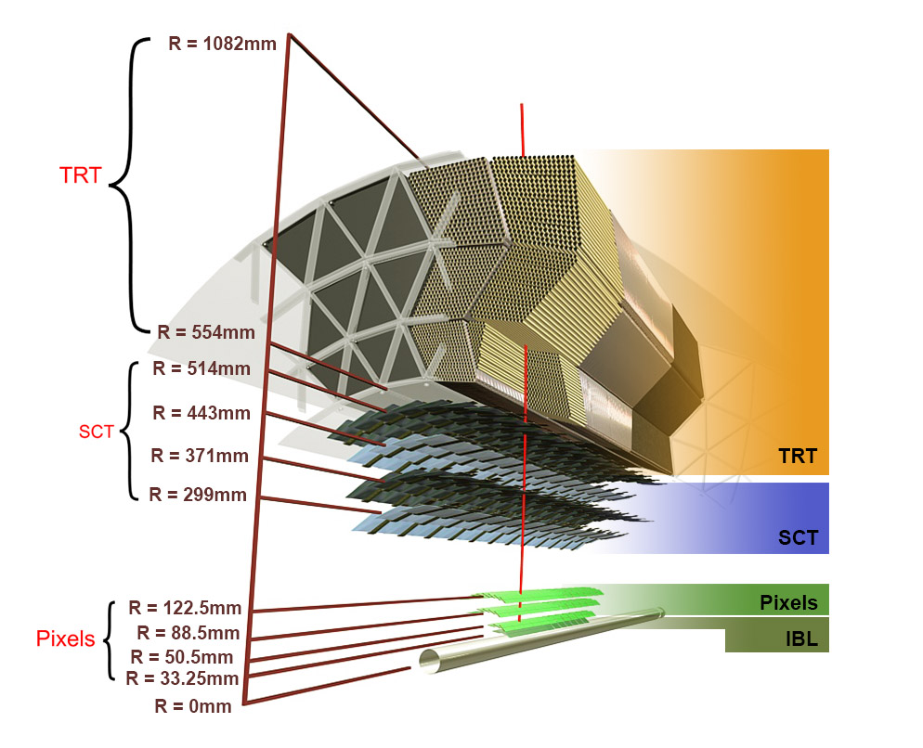
\includegraphics[width = 0.8\textwidth]{Chapter2/ATLAS_ID_Barrel}
	 \caption{Barrel part of ID of the ATLAS experiment with the IBL, Pixel, SCT and TRT sub-detectors~\cite{ATL-PHYS-PUB-2018-003, ATLAS:2020ixw}. }
	\label{fig:Chap2:ATLAS:ID_Barel}
\end{figure}

The ID is composed of four sub-detectors: The Insertable B-Layer (IBL), the Pixel Detector, 
the Semiconductor Tracker (SCT) and the Transition Radiation Tracker (TRT). 
%The different sub-systems are respectively described in Sections \ref{sec:Chap2:ID:B-Layer},
% \ref{sec:Chap2:ID:Pixel}, \ref{sec:Chap2:ID:SCT} and \ref{sec:Chap2:ID:TRT}.


%\begin{wrapfigure}{r}{0.5\textwidth}
%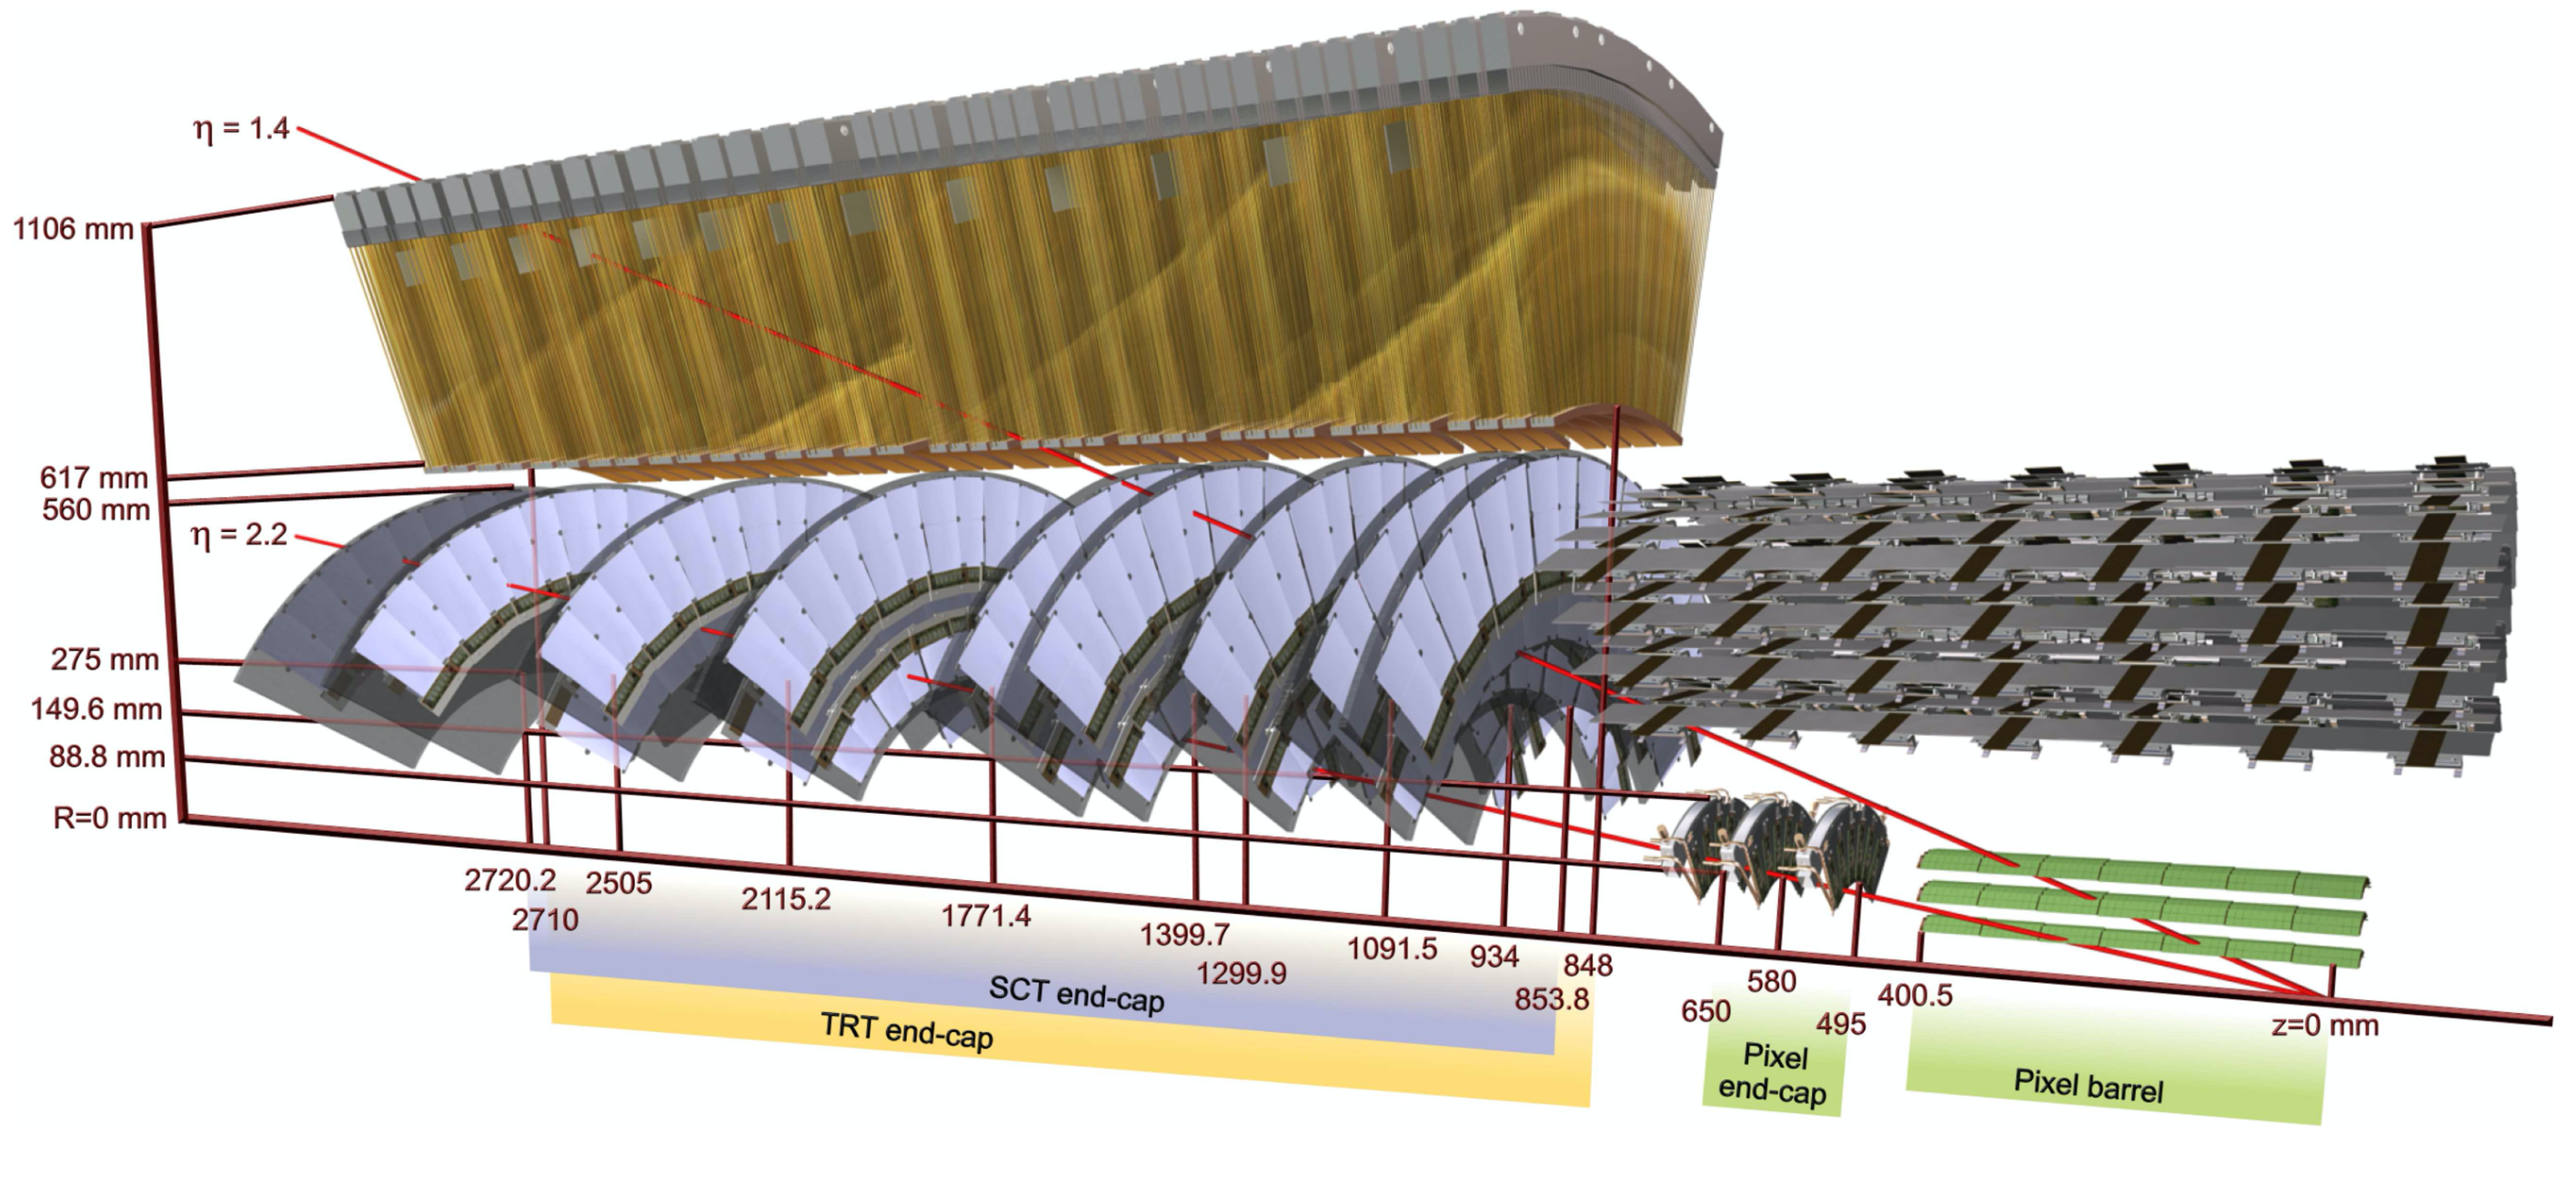
\includegraphics[width = 0.95\textwidth]{Chapter2/ATLAS_ID_TRT}
%\caption{End-cap and barrel of the ID.} \label{fig:Chap2:ID_Endcap}
%\end{wrapfigure} 

%Depending on the $\eta$ that a particle has, it will interact with some elements of the detector.
%Figure~\ref{fig:Chap2:ATLAS:ID_Endcap} shows the end-cap elements transversed by
%two charged particles with $\eta = 2.2$ and $1.4$. The track with $\eta = 1.4$ traveses first the beryllium beam-pipe, then the three
%cylindrical silicon pixels and the four disks with double layers of the SCT. Finally, this particle travels across approximately 40 tubes
%in the TRT wheels. In contrast, the particle with $\eta = 2.2$ encounter the first of the cylindrical silicon-pixel layers after leaving
%the beryllium pipe. Then, the two end-cap pixel disks and the four last disks of the end-cap SCT.

%\begin{figure}
%	\centering
% 	 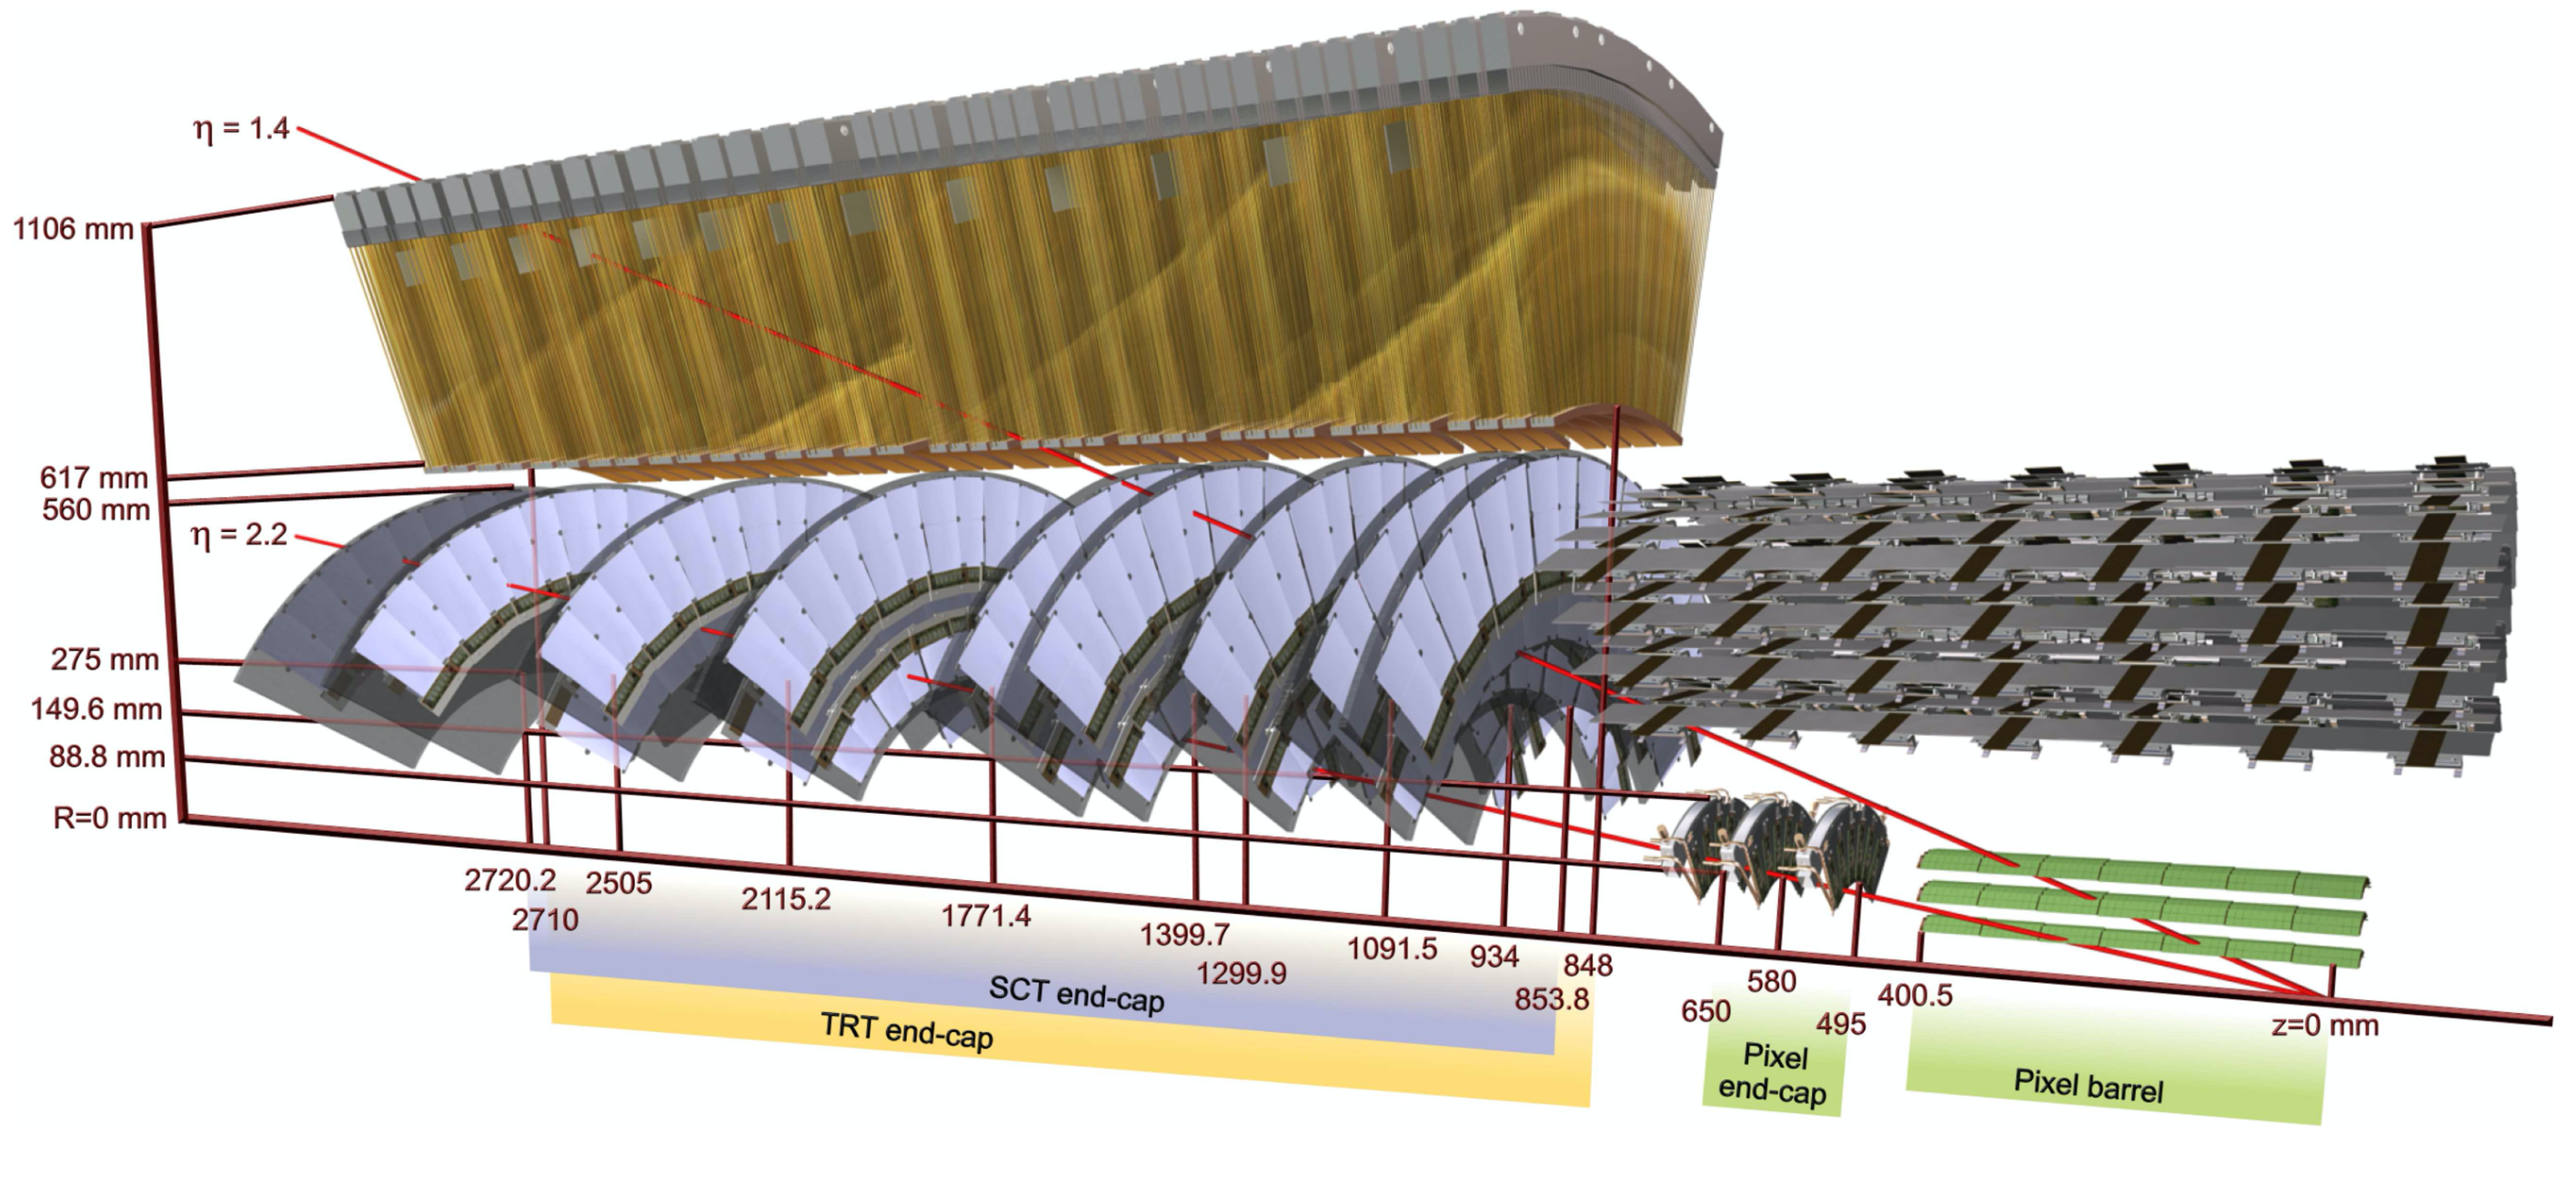
\includegraphics[width = \textwidth]{Chapter2/ATLAS_ID_TRT}
%	 \caption{End-cap of the ID.}
%	\label{fig:Chap2:ATLAS:ID_Endcap}
%\end{figure}

% Silicon semiconductors
%When a charged particle traverses a doped silicon semiconductor, it creates a pair electron-hole by ionisation.
%An electric field is applied to the active part of the detector module so that the electron drifts in oposite direction
%of the electric field and the hole in the field direction. Then, both charges are collected by the p-n junctions. 
%The silicon sensors can be shaped either as pixels, providing precies 2D space point, or as strips, giving
%a single dimension positioning.
%Of the order of $10^5$ electron-hole pairs are liberated when a particle crosses the silicon wafer and, with 
%appropriate electronics, a clear signal is obtained in the pixel or strip in which the charged was collected. 



% Electronics data https://atlas.cern/discover/detector/inner-detector
\paragraph{Insertable B-Layer}\mbox{}\\
\label{sec:Chap2:ID:B-Layer}
The IBL~\cite{Capeans:1291633} is the innermost component of the ID. It is located between the beam pipe and
the Pixel Detector.  Added after Run 1, it provides the closest-to-IP measurements. This improves the robustness 
and performance of the ATLAS tracking system. It plays a fundamental role in \btag
efficiency because this tagging relies on precise vertex reconstruction. %The IBL provides redundancy in the measurements 
%of tracks in order to control the fake rate arising from random combinations of clusters in events with a high pile-up background.
With a hit resolution of $8\,$\textmu m in $r$-$\phi$ and $40\,$\textmu m along $z$, the IBL covers the $|\eta| < 2.7$ and the entire $\phi$ range.

The IBL consists of pixel planar sensors and 3D pixel sensors~\cite{Capeans:1291633, LaRosa:2016nbd} mounted on 
280 silicon pixel modules and arranged on 14 azimuthal staves.

%The barrel structure if the IBL has a radius of $3.3\,$cm and is composed by 14 carbon fibre 
%staves as it is shown in Figure~\ref{fig:Chap2:ATLAS:ID_IBL}.
%Each stave has incorporated cooling CO$_2$ circuits and contains 20 modules.
%They use two types of photodetectors: ATLAS pixel planar sensors and 3D pixel sensors~\cite{LaRosa:2016nbd}.. 
%The used pixels have a size of $50 \times 400$ \textmu m$^{2}$  %, providing a resolution of the order of 100 \textmu m. 
%Due to the high luminosity of the LHC, the IBL is built with radiation-tolerant sensors.

%\begin{figure}
%	\centering
% 	 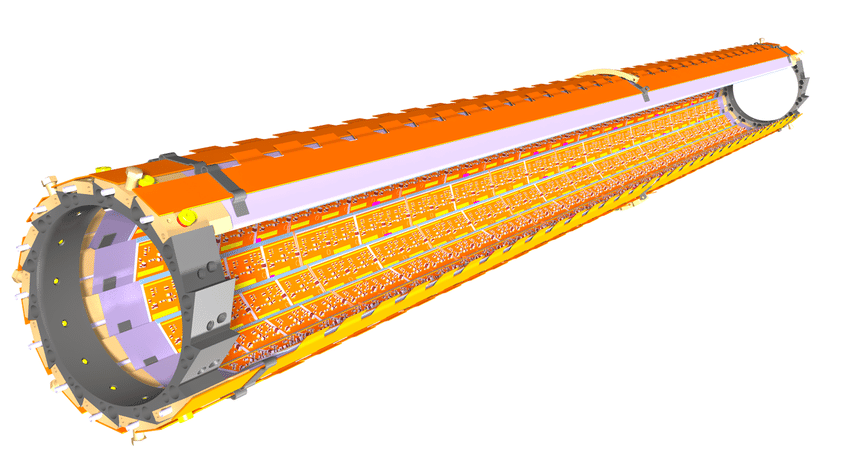
\includegraphics[width = 0.8\textwidth]{Chapter2/ATLAS_ID_1_IBL}
%	 \caption{Schematic drawing of the ATLAS IBL Detector~\cite{Capeans:1291633}. \pablo{If material had to be removed, this is a candidate.}}
%	\label{fig:Chap2:ATLAS:ID_IBL}
%\end{figure}

%\subsubsection{Pixel Detector}
\paragraph{Pixel Detector}\mbox{}\\
\label{sec:Chap2:ID:Pixel}
The ATLAS Pixel Detector~\cite{CERN-LHCC-2017-021} is made up of four layers of silicon pixels 
of $50 \times 400\,$\textmu m$^{2}$ organised in modules. The barrel modules are arranged in three cylinders
concentric to the beam axis %\footnote{The cylinders concentric to axis along beam the beam are referred as the barrel.} 
and three concentric disks at both ends of the barrel. %as Figure~\ref{fig:Chap2:ATLAS:ID_PixelDetector} shows.
%As well as the IBL, it aims to reconstruct the trajectories of the particles traversing it.
Each of these modules consists on a silicon pixel sensor bonded to the front-end electronic chips.
It provides full coverage of the azimuthal angle $\phi$ and a pseudorapidity range of  $|\eta| < 2.5$ as well as
a resolution of $10\,$\textmu m in $r$-$\phi$ and $115\,$\textmu m in the $z$-axis.

%The Pixel Detector and the IBL combined contain $92 \times 10^6$ pixels with its respective electronic channels, which
%cover an area of approximately $1.9\,$m$^2$ of silicon consuming $15\,$kW.
%The barrel region consists of four concentric layers equipped with 1736 sensor modules and each 
%of the two end-caps has three disks with 2888 modules~\cite{ATLAS_Web_Detectors}. Figure
%\ref{fig:Chap2:ATLAS:ID_PixelModule} shows the assembly view and cross section of a module of the ATALS 
%ID Pixel Detector. 

%Hits in a pixel are read out if the signal exceeds a tunable threshold. The pulse height is measured using 
%the Time-over-Threshold (ToT) technique.

%\begin{figure}
%	\centering
%	 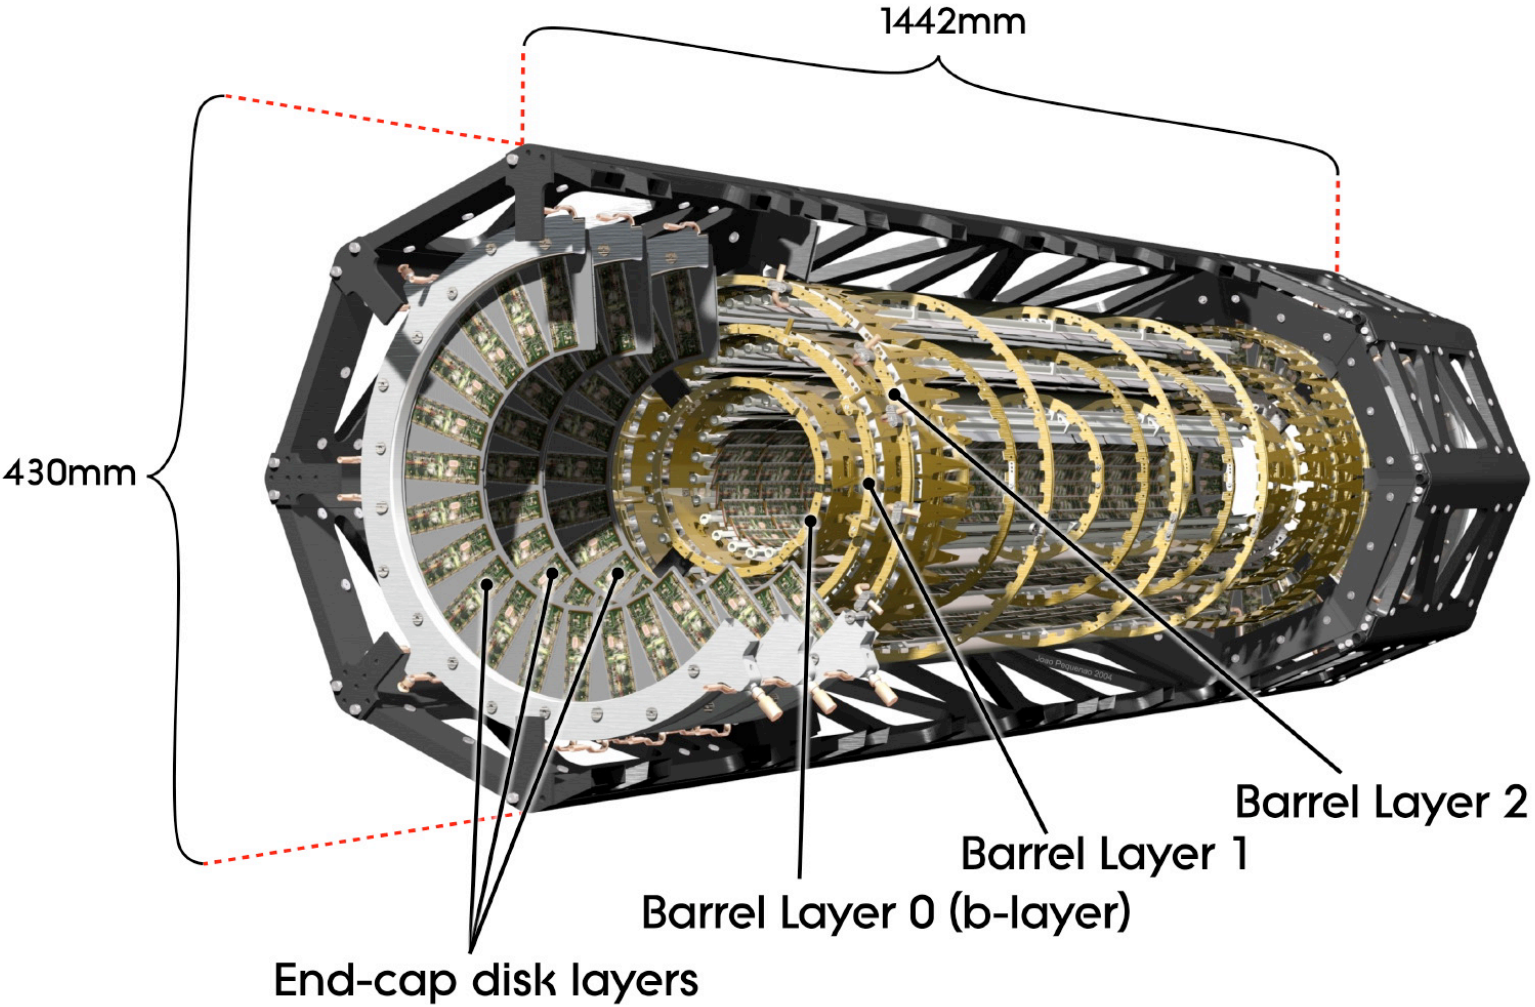
\includegraphics[width = 0.8\textwidth]{Chapter2/ATLAS_ID_2_PixelDectector}
%	 \caption{Schematic view of the ATLAS Pixel Detector consisting of individual barrel and end-cap layers~\cite{ATLAS:2008xda}.}
%	\label{fig:Chap2:ATLAS:ID_PixelDetector}
%\end{figure}



%\subsubsection{Semiconductor Tracker}
\paragraph{Semiconductor Tracker}\mbox{}\\
\label{sec:Chap2:ID:SCT}
The SCT consists of 4088 modules tiling four coaxial cylindrical layers in the barrel region and two end-caps each containing nine disk
layers, all of these surrounding the Pixel Detector. %and providing additional precision tracking.~\cite{Ahmad:2007zza}
%The main difference with the Pixel Detector is that 
The SCT uses microstrip sensor technology. %A microstrip is very similar to a pixel but much larger length ($6\,$cm) in one direction. 
The reason to use microstrips instead of pixels is that the strips are more cost-effective than traditional pixels and a 
good spatial resolution can be obtained as well if the strips are arranged with an angular offset. Therefore, each SCT detector 
unit consists of two back-to-back silicon-microstrip planes with a relative angle of $40\,$mrad.
Eight strip layers (i.e. four space points) are crossed by each track in the SCT providing valuable tracking information with a resolution of 
$17\,$\textmu m in $r$-$\phi$ and $580\,$\textmu m in the $z$ coordinate. The SCT covers the entire $\phi$ range and up to $|\eta| <2.5$.

%Figure~\ref{fig:Chap2:ATLAS:ID_SCT} shows an exploded view of the different components of an SCT module, including 
%the high termal conductivity spine, the polyimide hybrids and readout chips.

%\begin{figure}
%	\centering
 %	 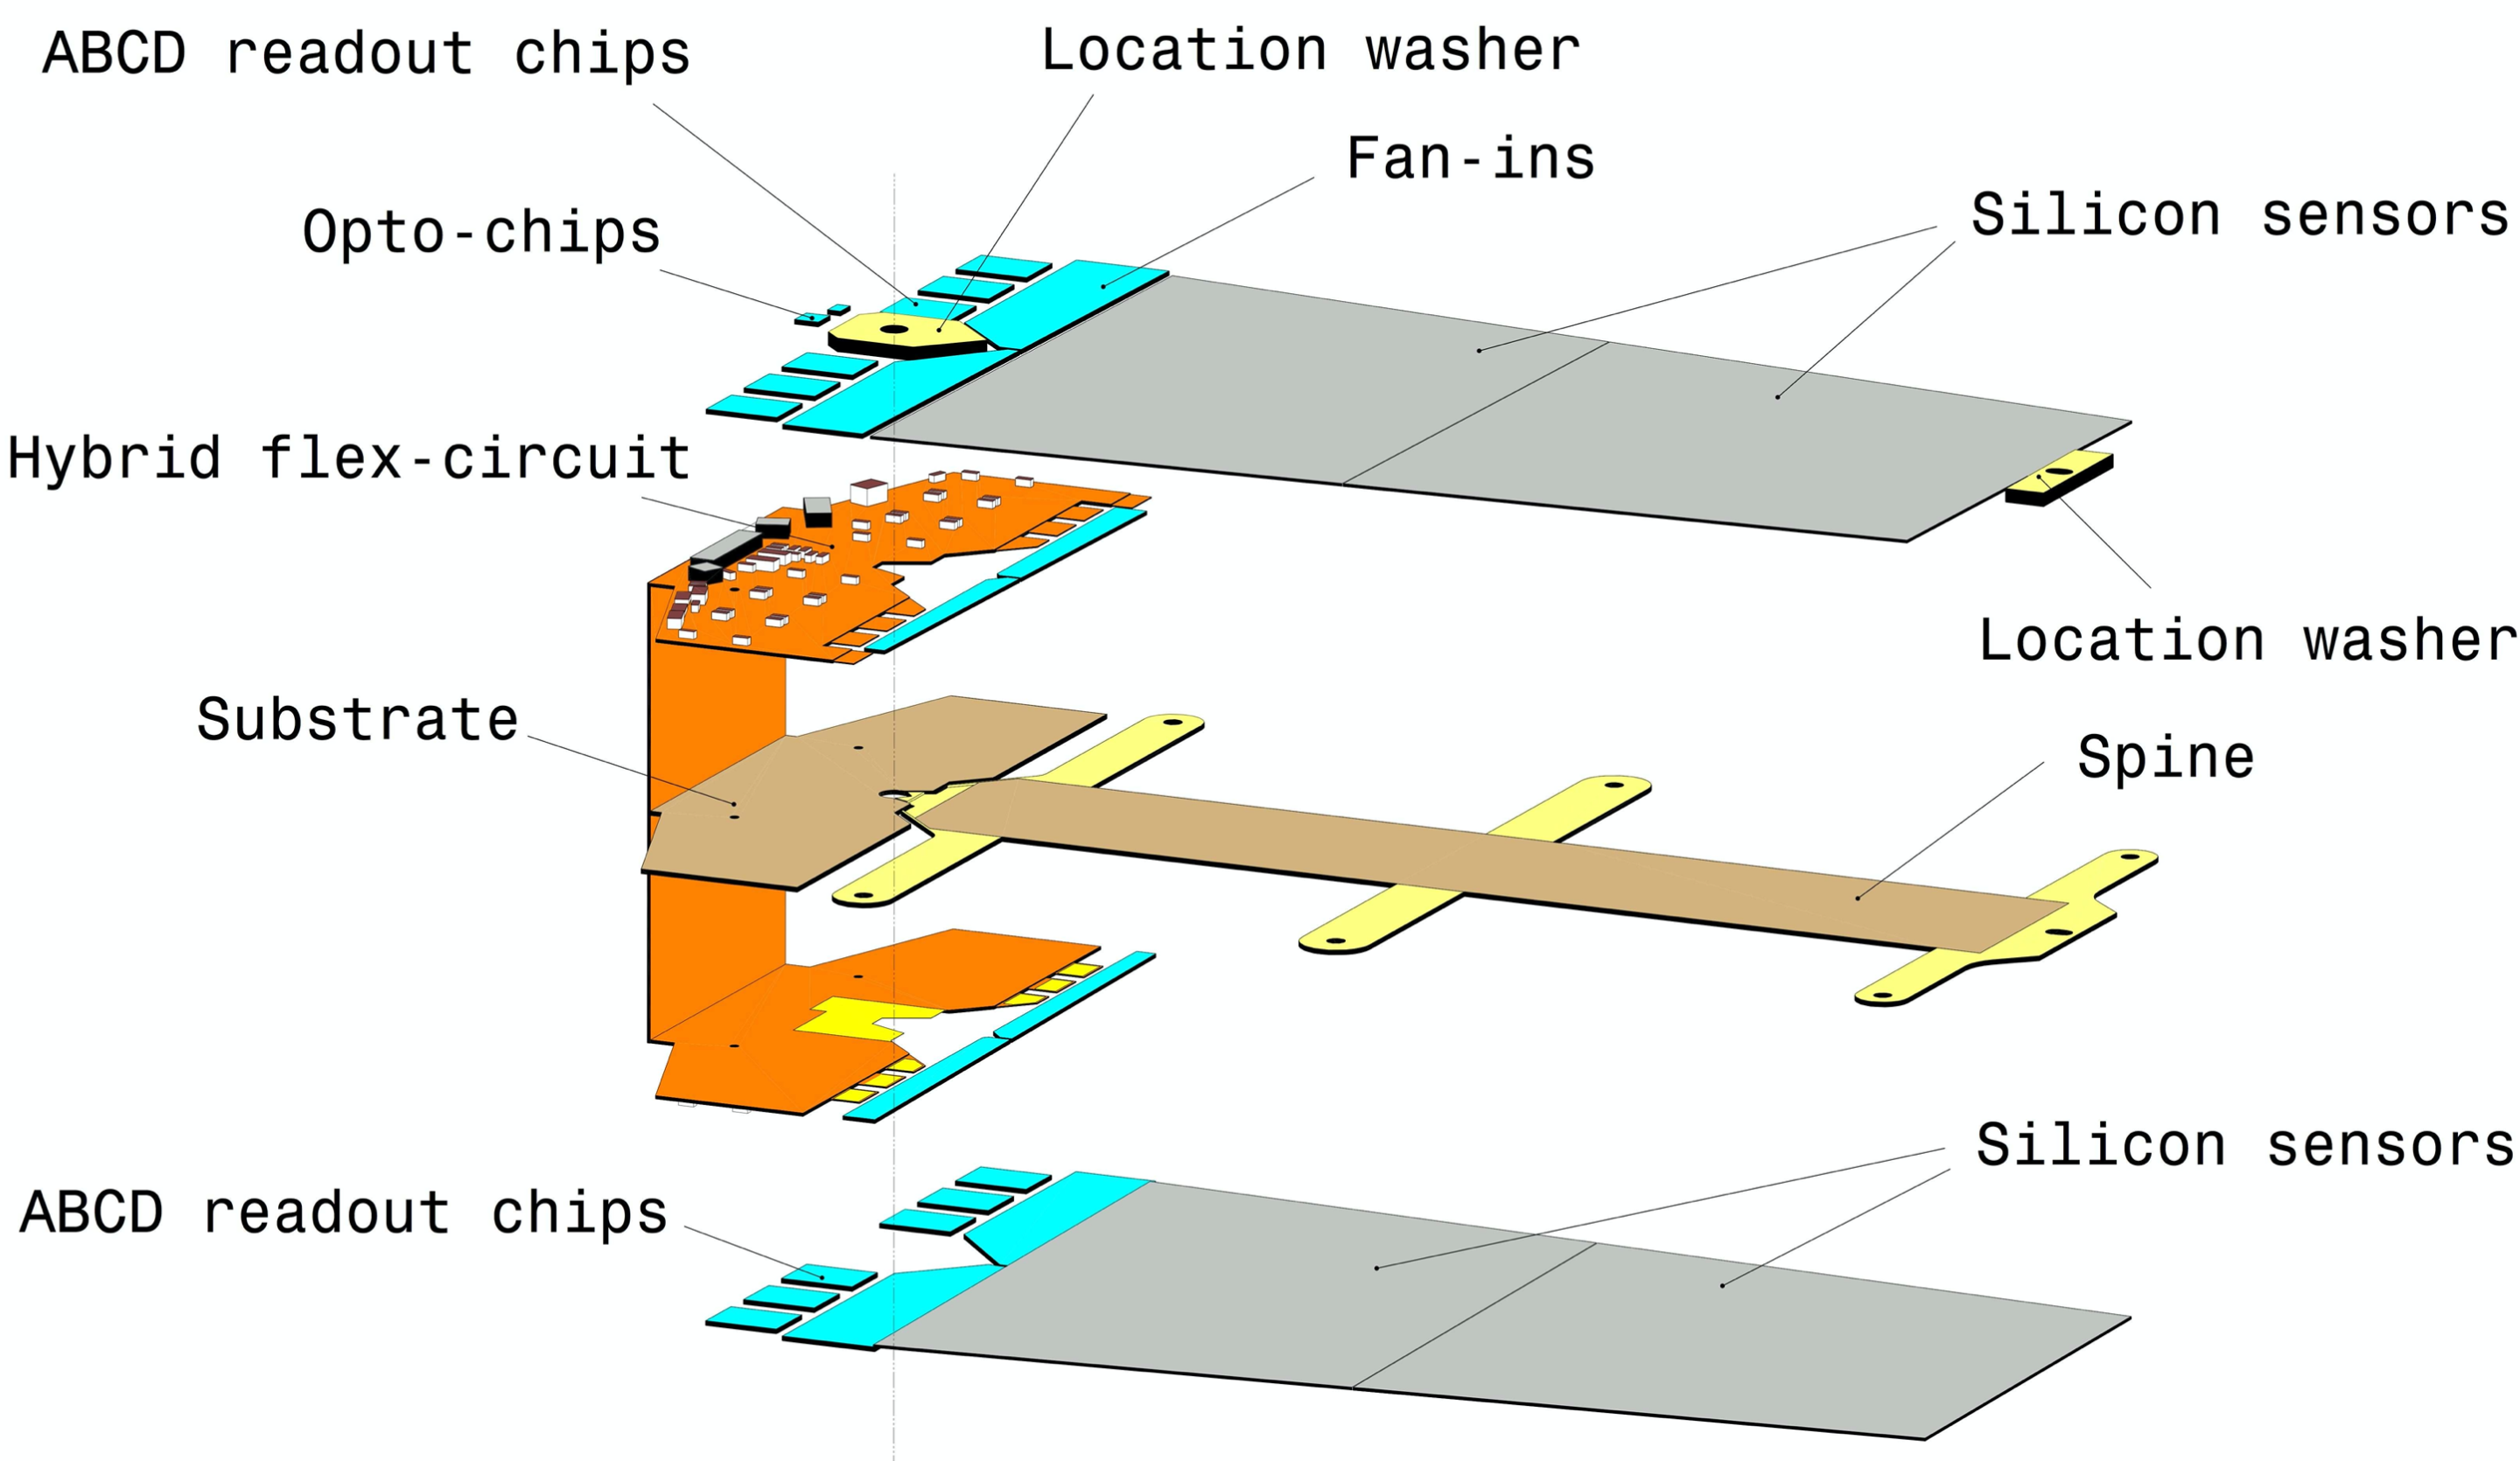
\includegraphics[width = 0.8\textwidth]{Chapter2/ATLAS_ID_SCT}
%	 \caption{Schematic view of an SCT detector module~\cite{ATLAS:2008xda}.}
%	\label{fig:Chap2:ATLAS:ID_SCT}
%\end{figure}

%\begin{figure}
%\centering
%\begin{minipage}{.4\textwidth}
%	\centering
% 	 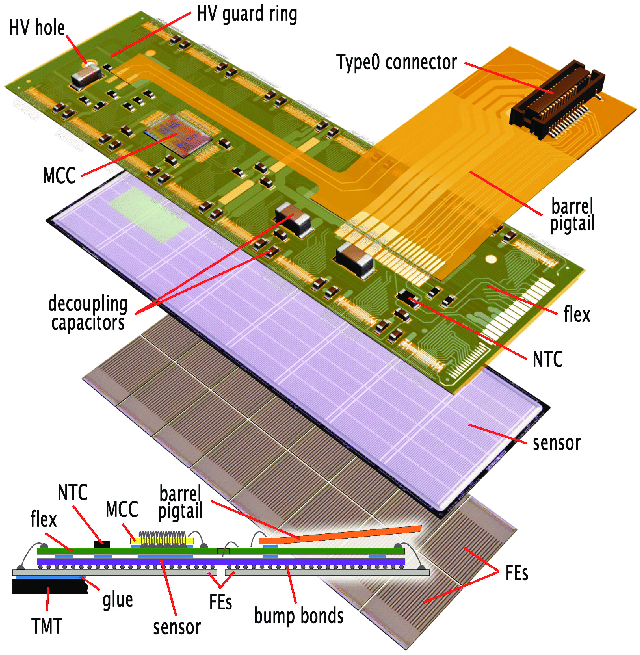
\includegraphics[width = \textwidth]{Chapter2/ATLAS_ID_PixelModule}
%	 \captionof{figure}{Pixel Detector module~\cite{CERN-LHCC-2017-021}.}
%	\label{fig:Chap2:ATLAS:ID_PixelModule}
%\end{minipage}%
%\begin{minipage}{.6\textwidth}
%	\centering
% 	 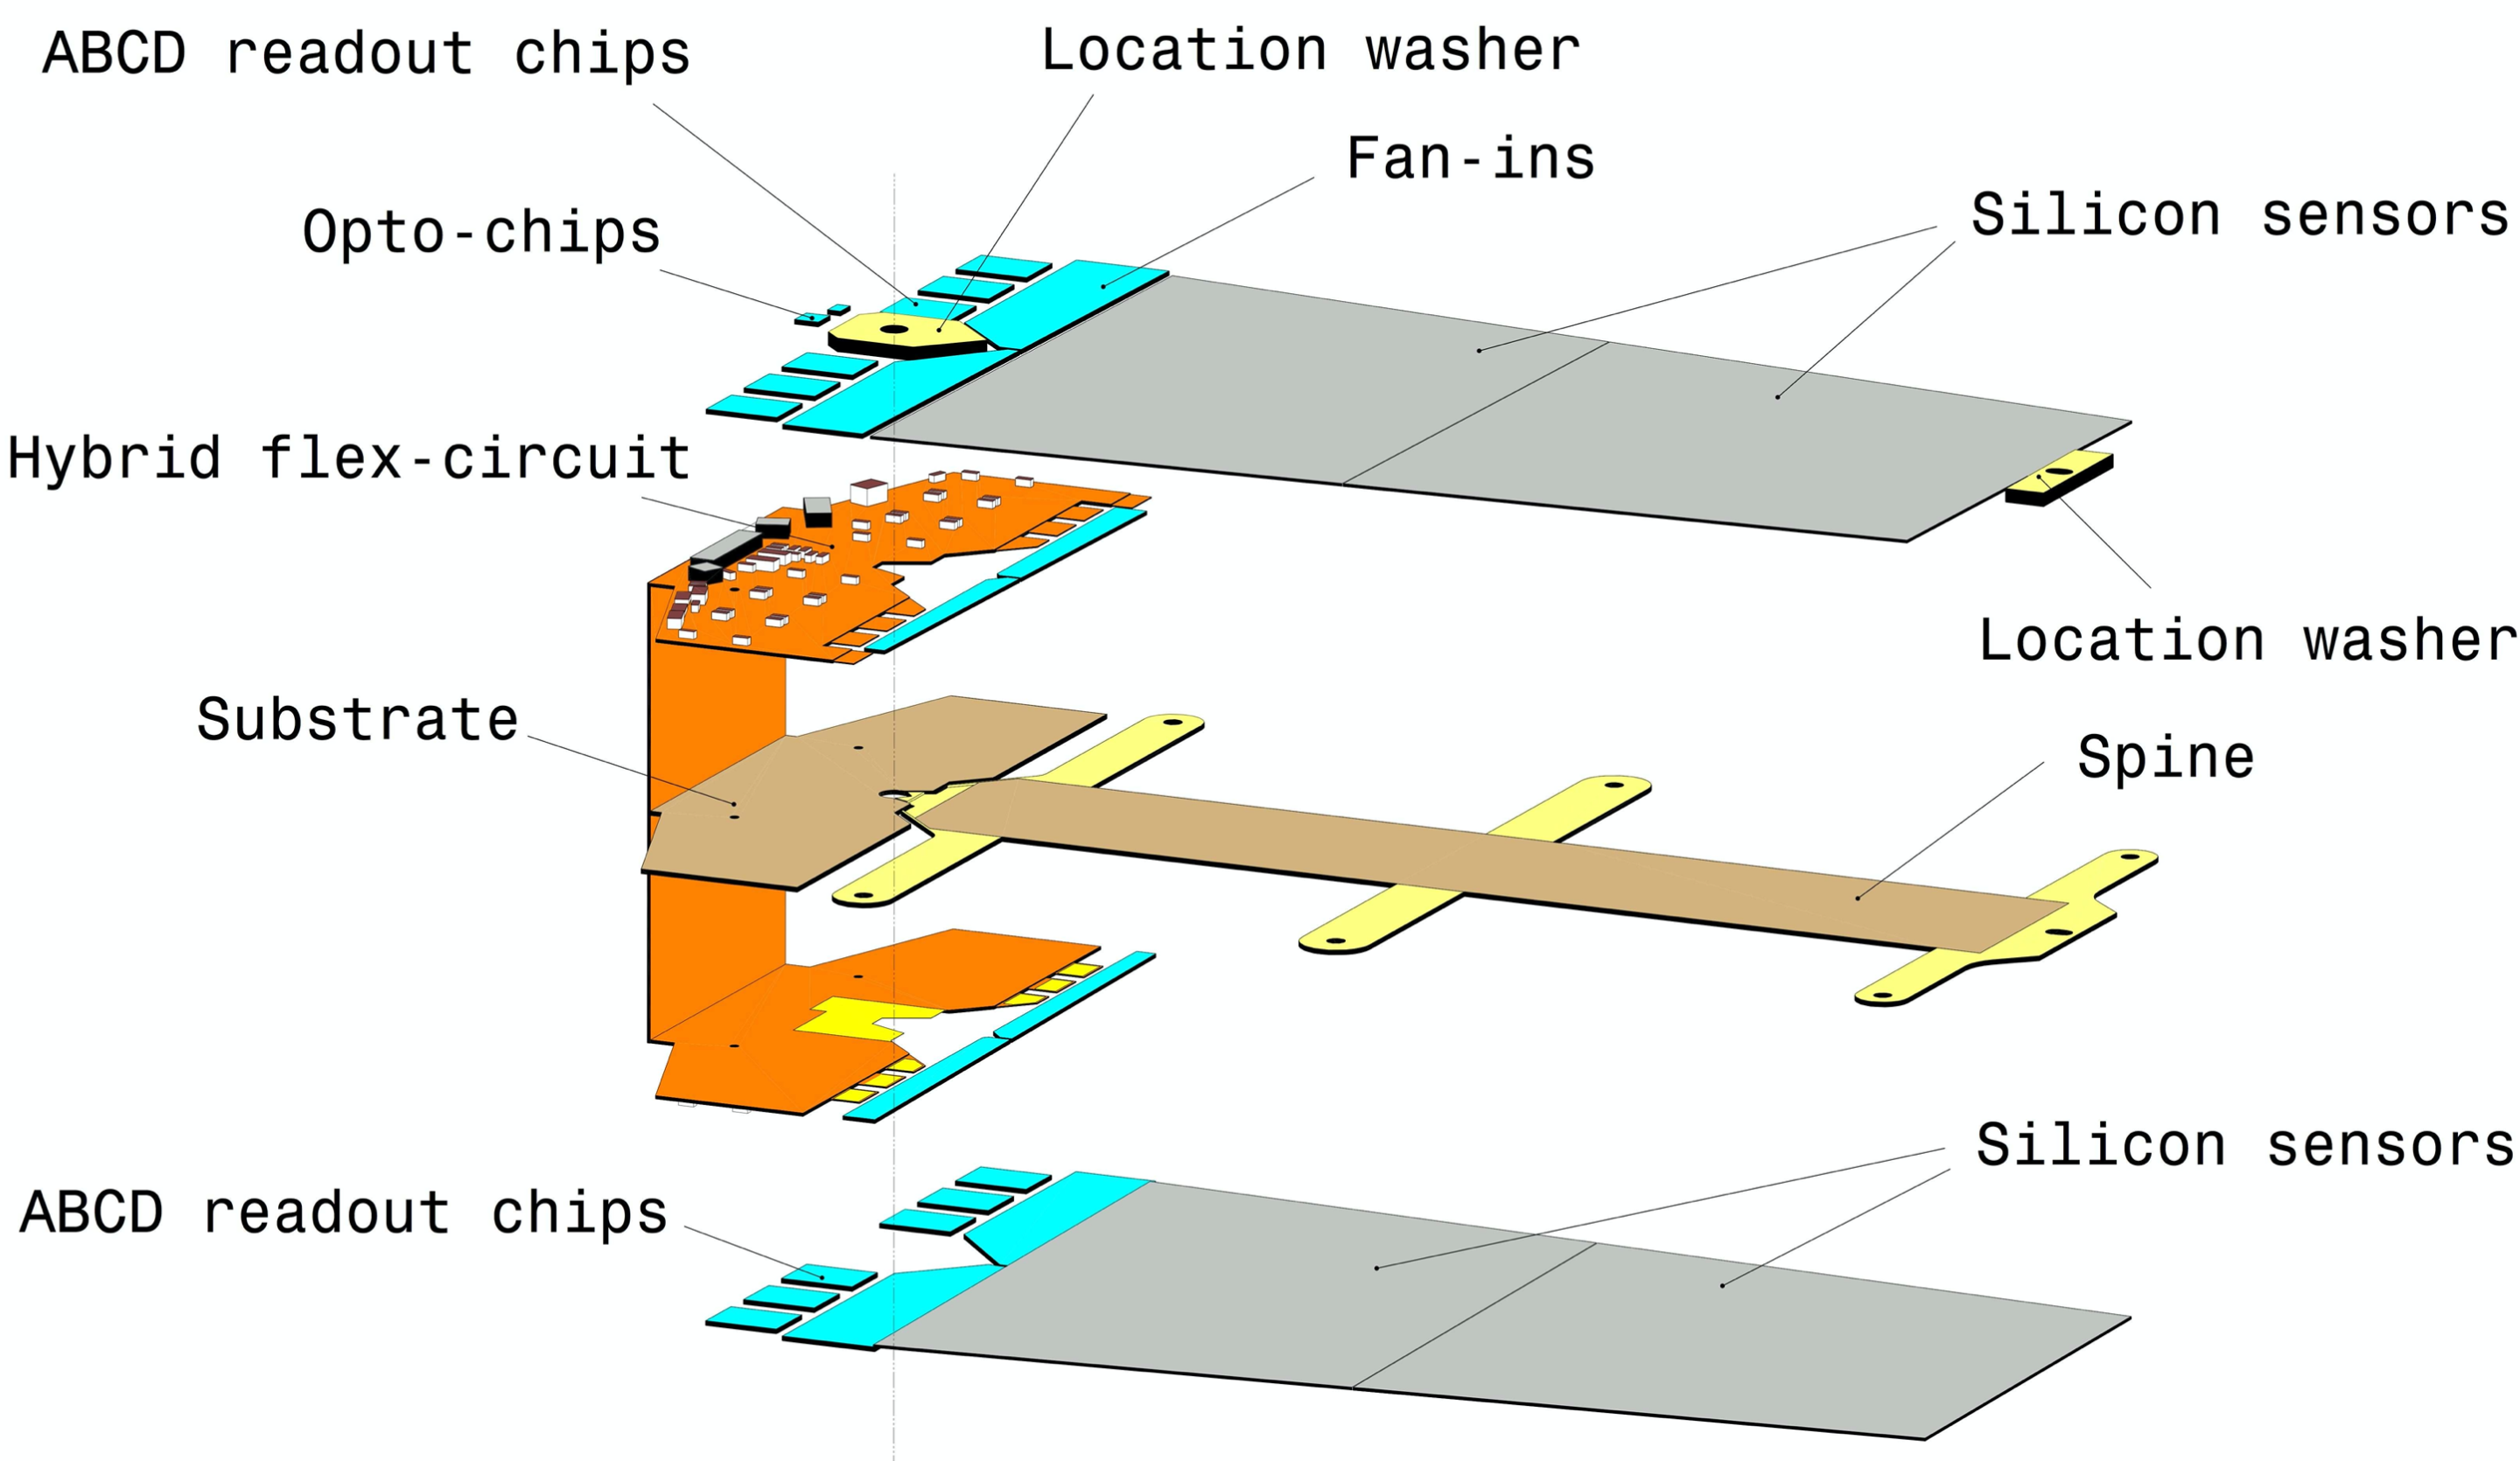
\includegraphics[width = \textwidth]{Chapter2/ATLAS_ID_SCT}
%	 \captionof{figure}{SCT detector module~\cite{ATLAS:2008xda}.}
%	\label{fig:Chap2:ATLAS:ID_SCT}
%\end{minipage}
%\end{figure}




%\subsubsection{Transition Radiation Tracker}
\paragraph{Transition Radiation Tracker}\mbox{}\\
\label{sec:Chap2:ID:TRT}
The TRT is used in conjunction with the Pixel Detector and silicon micro strip (SCT). %to extend 
%the $\eta$ range in which the tracks can be reconstructed up to $|\eta| = 2$. 
This part of the ID 
is formed by about 300000  straw tubes with  $4\,$mm diameter filled with gas.
 The TRT relies both on the collection of both primary and secondary ionisation charges arising 
 from the transition radiation to measure the  track of charged particles. 
 The tube surface functions as cathode while the wire in the centre as anode. When a charged particle passes through the Xe-based gas mixture in 
 the tube, it ionises the gas and the freed electrons drift towards the anode, generating an electrical current. This detector provides 
 a single hit resolution of $130\,$\textmu m in $r$-$\phi$ but does not have sensitivity in $z$.
%resolution of 130 μ m
The TRT also provides discrimination between electrons and pions since the latter generates a smaller signal than the former. 
%When the electrons pass, they produce
%x-ray photons that lead to strong avalanches within the tubes and, thus, a great signal.
% They use mostly Xe gas but, for leaks, Ar is used instead for budget reason

Table~\ref{tab:Chap2:ID:Detalils} summarises the main characteristics of the 
ID subdectectors. 

\begin{table}[h!]
\centering
\begin{tabular}{c c c }
\toprule
Subdetector 	& Element size (\textmu m) 	& Intrinsic resolution (\textmu m) 	\\ \midrule
IBL 			&   $50 \times 250$		&   $8 \times 40$			\\
Pixel 		&   $50 \times 400$		&   $10 \times 115$			\\
SCT 			&   	    80				&   $17 \times 580$			\\
TRT 			& 	  4000			&   $130$					\\ \bottomrule 
\end{tabular}
\caption{Overview of the main features of the ID subdetectors. The intrinsic resolution of the 
IBL, the Pixel and SCT is provided for borh $r$-$\phi$ and $z$ directions, while for TRT subdetector
only along $r$-$\phi$.}
\label{tab:Chap2:ID:Detalils}
\end{table}



%%%%%%%%%%%%%%%
%          Calorimeters           %
%%%%%%%%%%%%%%%
\subsection{Calorimeters}
\label{sec:Chap2:CALO}
After the ID, the next layer of detectors in the ATLAS machine corresponds to the calorimeters (see Figure~\ref{fig:Chap2:ATLAS:Calorimeters})~\cite{Cavallari_2011}. 
Their purpose is to measure the energy of the particles 
(neutral or charged), as well as to help the ID to reconstruct the path followed by them. 
Most particles initiate a shower when they enter into the calorimeter. 
Either all or part of the energy 
of these particles is deposited in the device and measured.
Most of calorimeters in particle physics are segmented transversely to provide information about the direction of the particles.
Based on the shower shape, the longitudinal segmentation provides information for particle identification.
%(a more detailed discussion is presented in Chapter \ref{chap:ObjectReconstruction}). 

The ATLAS detector has two types of calorimeters depending of the type of particles that it is desired to detect: 
the electromagnetic calorimeter (ECAL), which measures the energy of electrons/positrons and photons, 
and the hadronic calorimeter (HCAL), which registers the energy of the strongly-interacting particles. 
%Both classes are covered in the next sections.

Calorimeters are typically categorised into two types: sampling and homogeneous. 
Sampling calorimeters are constructed from two types of materials (passive and active), 
while homogeneous calorimeters are made from a single type. 
Both the ECAL and HCAL are sampling calorimeters, which consist of alternating layers of different materials.

%\begin{itemize}
%	\item \textbf{Passive material}: Also known as absorber, it is a denser material to full stop the traversing particles.
%		When a particle interacts with the passive material it produces the shower (Figures \ref{fig:Chap2:ATLAS:PShoweringSim} 
%		and \ref{fig:Chap2:ATLAS:PShowering}).
%		For the absorber layers in ATLAS, lead is used for the ECAL and steel for the HCAL.
%	\item \textbf{Active material}: This material detects the particles from the shower originated in the absorber.
%		The liquid Argon (LAr) is used as active material for ECAL and plastic scintillator for HCAL.
%\end{itemize}
%In the homogeneous calorimeters, the material used combines the features of an absorber and a detector, performing both tasks.

\begin{figure}
	\centering
 	 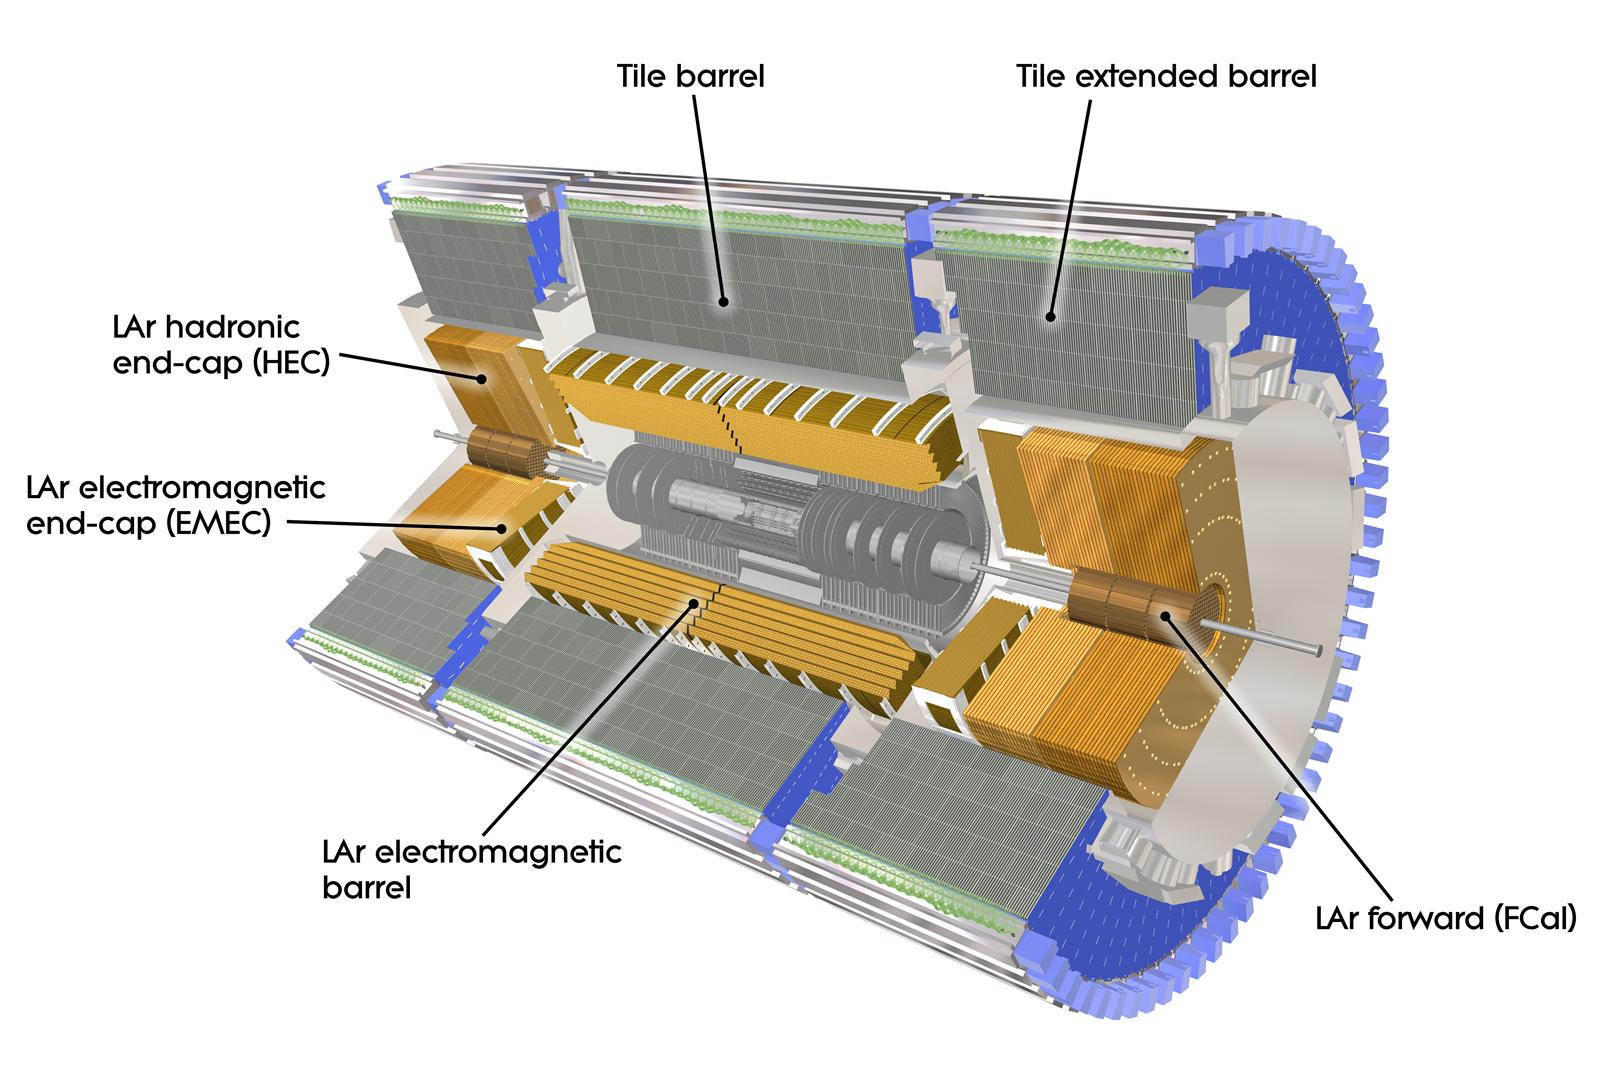
\includegraphics[width = 0.9\textwidth]{Chapter2/ATLAS_Calorimeters}
	 \caption{Computer generated image of the ATLAS calorimeters~\cite{ATLAS_Web_Detectors}.}
	\label{fig:Chap2:ATLAS:Calorimeters}
\end{figure}

%\paragraph{Scintillator}\mbox{}\\
%The particles from the shower leave some of the molecules of the plastic scintillator in an excited state. The 
%subsequent decay of these molecules produces the emission of photons in the ultraviolet energy region.
%This light is collected by photomultiplier tubes at the edge of the tiles
%and converted into a current pulse whose amplitude is proportional
%to the energy deposited by transversing particle.


%The plastic scintillators turn the particles that the shower
 %originated in the steel layer into photons, which are converted into an electric current whose intensity is proportional to the original particle's intensity 


%%%%%%%%%%%%%%%
%         Particle shower        %
%%%%%%%%%%%%%%%
%\subsubsection{Particle showering}
%\label{sec:Chap2:CALO:Shower}

%\pablo{The whole Section~\ref{sec:Chap2:CALO:Shower} could be removed but I rather not.}

%A particle shower is a cascade of secondary particles produced when a high-energy particle interacts with matter.
%The first particle interacts with the passive material producing a secondary particle with less energy than the first one.
%The second particle
%does the same and, in each step, the particles produced are less and less energetic. For a single incoming particle, 
%this process can continue for thousands of iterations~\cite{grupen_shwartz_2008}. An illustration of the
%EM and hadronic particle cascades is shown in Figure~\ref{fig:Chap2:ATLAS:PShoweringSim}.

%\begin{figure}
%\centering
%\begin{minipage}{.45\textwidth}
%	\centering
% 	 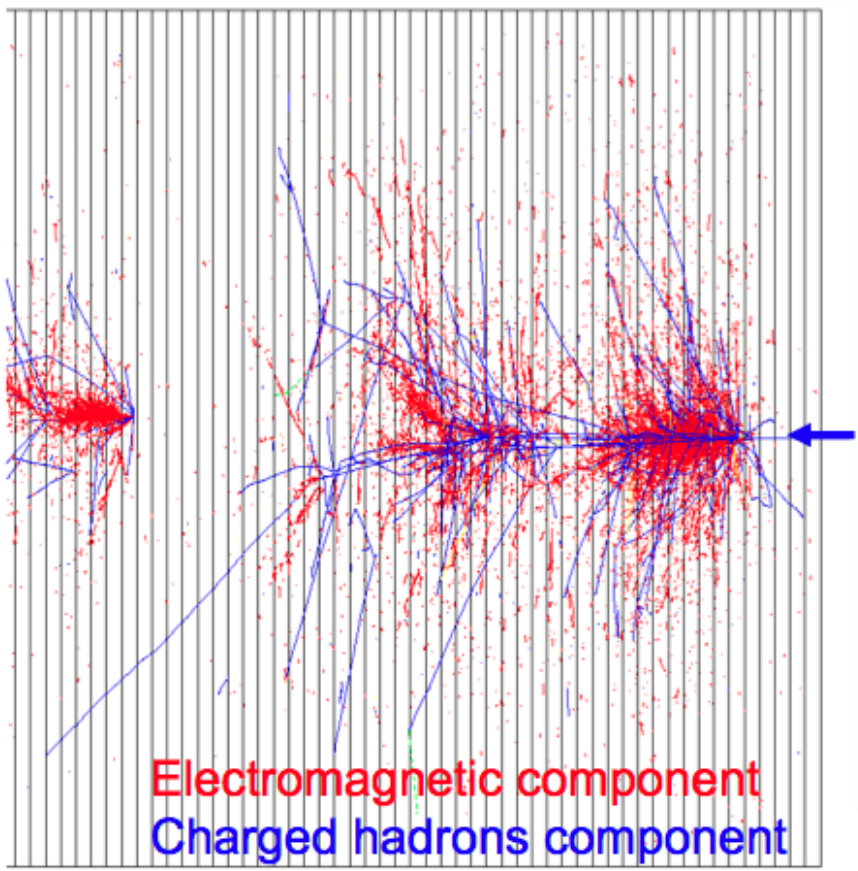
\includegraphics[width = 0.8\textwidth]{Chapter2/Showering_simulation}
%	 \caption{EM and hadronic cascades.}
%	\label{fig:Chap2:ATLAS:PShoweringSim}
%\end{minipage}%
%\begin{minipage}{.55\textwidth}
%	\centering
% 	 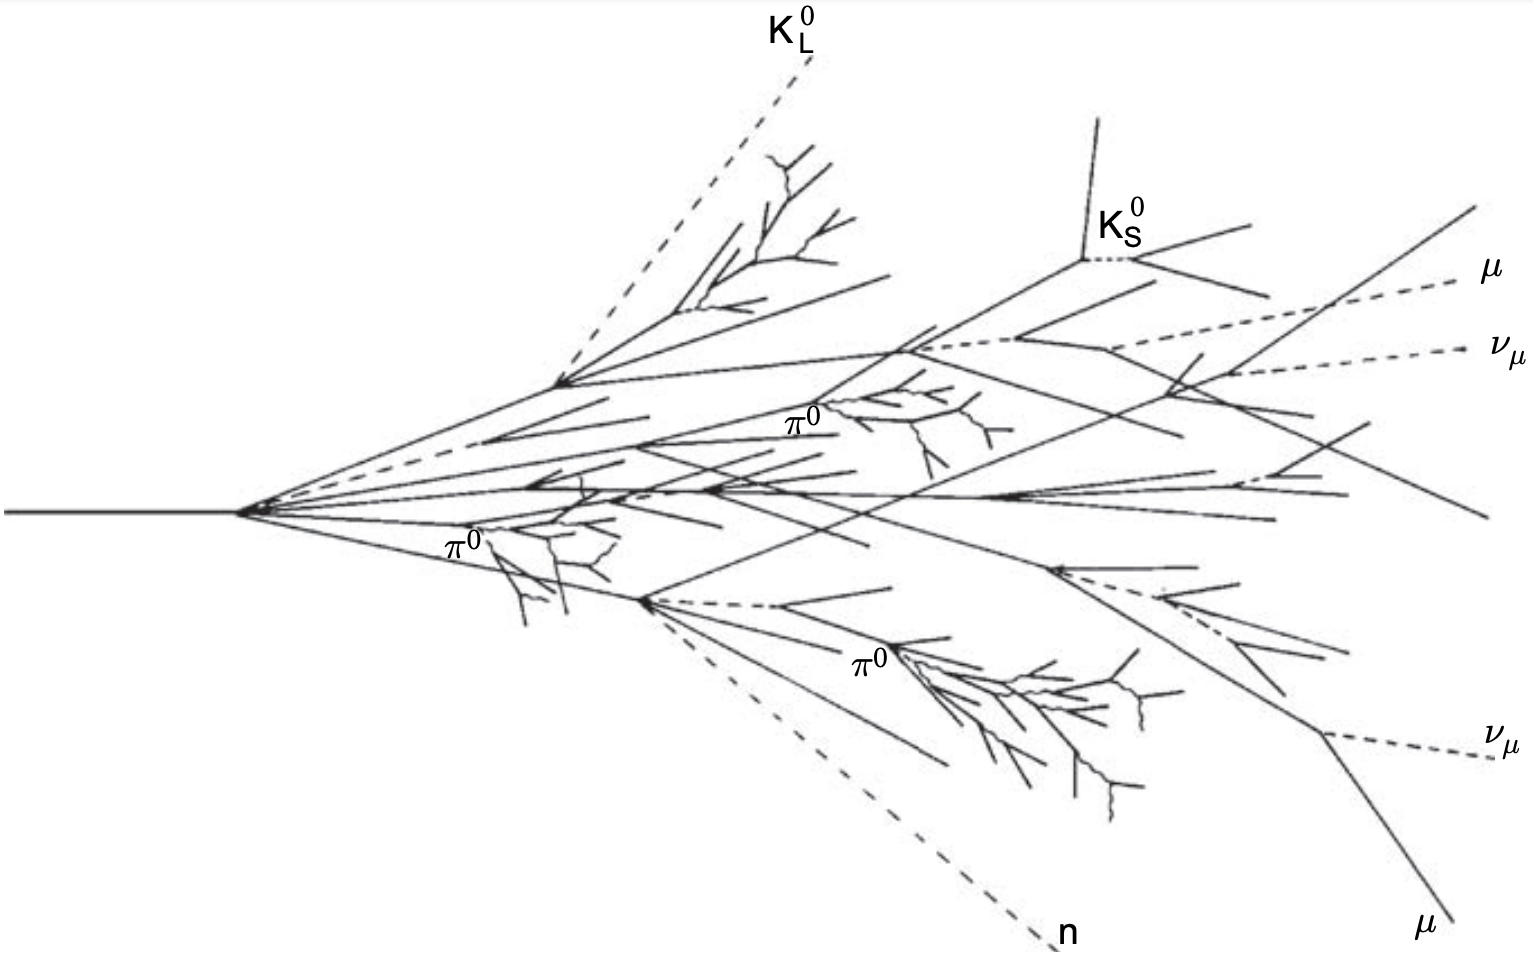
\includegraphics[width = 0.85\textwidth]{Chapter2/ShoweringHAD_Feynman}
%	 \caption{Sketch of a hadronic cascade~\cite{grupen_shwartz_2008}.}
%	\label{fig:Chap2:ATLAS:PShowering}
%\end{minipage}
%\end{figure}

\begin{comment}
\paragraph{Electromagnetic shower}\mbox{}\\
The electromagnetic (EM) shower is initiated by a $\Pelectron$, $\APelectron$ or  $\Pphoton$, these three particles are the sole components of this type of shower.
At energies higher than 100 MeV, the EM showering is based on two main processes: bremsstrahlung and pair production.
The electrons lose their energy almost exclusively by bremsstrahlung radiation, a process in which the lepton radiates thousands of soft photons because of its
interaction with another charged particle.
The photons lose their energy by the production of an $\Pelectron$$\APelectron$ pair.
At lower energy scales, other processes contribute. In the MeV range, the Compton scattering\footnote{Scattering of a photon after interacting with a charged particle, usually an electron.}
and photoelectric effect\footnote{Emission of photoelectrons when the EM radiation interacts with matter.} are the dominant interactions for energy loss
for photons, while the ionisation and excitation are for the charged particles ($\Pelectron$ and $\APelectron$).


\paragraph{Hadronic shower}\mbox{}\\
When a hadron interacts with the passive material, this shower is initialised. % and it always has an EM component too. 
Both strong and EM interactions are involved in the development of this type of shower and 
they present a larger variety of particle components. Therefore, the hadronic showers are significantly more 
complex than the EM. Figure~\ref{fig:Chap2:ATLAS:PShowering} shows the processes leading to a hadronic cascade.

The production of neutral pions represents about a third of the energy loss of hadronic interactions. These pions 
decay 98.8\% of times to two photons~\cite{Workman:2022ynf} that are starting the EM showers. The rest of hadronic interactions
consist of the production of charged mesons, nuclear fragments and protons, and soft neutrons and photons or 
unpredictable  loss through undetectable processes.
%~\cite{pdgPi0}
\end{comment}

%%%%%%%%%%%%%%%%%
%         Electric calorimeter        %
%%%%%%%%%%%%%%%%%
\subsubsection{Electromagnetic calorimeter}
\label{sec:Chap2:CALO:ECAL}
The ECAL~\cite{Cavallari_2011} absorbs the energy of the electrons ($\Pelectron$), 
positrons ($\APelectron$) and photons ($\Pphoton$) covering a pseudorapidity range 
of $|\eta|<1.475$ in the barrel. It is made of a lead absorber and the liquid Argon 
(LAr) as an active medium following an accordion shape. %, as can be seen in Figure~\ref{fig:Chap2:ATLAS:ECal},
%where the different layers are clearly visible. 
The shower originated in the absorber layer ionises the LAr producing a measurable current proportional to the energy of the original particle. 
The LAr layer operates at $89.3\,$K to maintain a pressure of $1\,$bar\footnote{The minimum to avoid the freezing of liquid argon in the region of the heat exchangers is $87.3\,$K.}~\cite{CERN-LHCC-96-041}. %\pablo{(en varios sitios pone lo de 87K pero no se explica por qué)}
The barrel part is split into two identical half-barrels separated by a small gap at $z=0$. 
Each end-cap calorimeter is composed of two coaxial wheels that cover $1.375|\eta|<3.2$. 

The total amount of material in the ECAL corresponds to 25-35 radiation lengths\footnote{The radiation 
length is characteristic of each material and corresponds mean distance 
over which a high-energy electron lose its energy by a factor $e=2.71828$ 
due to bremsstrahlung.} over the entire $\eta$ range.

%The total amount of material in the ECAL corresponds to 25-35 radiation lengths, $X_0$, and 2-4 nuclear interaction 
%lengths, $\lambda$, over the entire $\eta$ range. The ration length is characteristic of each material and corresponds mean distance 
%over which a high-energy electron lose its energy by a factor $e=2.71828$ due to bremsstrahlung. 
%The radiation length is the mean free
%path between interactions required to reduce the number of relativistic charged particles by the factor $1/e = 0.37$ as 
%they pass through matter. 

The energy resolution of a calorimeter can be parametrised as:
\begin{equation*}
	\frac{\sigma_E}{E}= \frac{a}{\sqrt{E}} \oplus \frac{b}{E} \oplus c \, ,
\end{equation*}
where $a$ is the stochastic term, $b$ the electronic noise $c$ is a constant that includes detector instabilities and
miscalibrations, and $E$ is the energy. The stochastic term considers the statistical fluctuations in the shower detection. This term
is larger for sampling calorimeters than for the homogeneous ones. The effect of $a$ diminishes with
increasing energy. The noise component $b$ of energy resolution arises from the noise %~\cite{TarekAbouelfadlMohamed2020}
of readout chain and varies with detector technique and readout circuit properties (e.g., detector capacitance, cables). The noise contribution 
also increases with decreasing energy of the incident particles. Finally, the constant term does not involve energy-dependent 
contributions and originates mainly from instrumental effects that cause variations in calorimeter response.
For the ECAL, the resolution is:
\begin{equation*}
	\frac{\sigma_E}{E} = \frac{10\%}{\sqrt{E}} \oplus \frac{170\textrm{ MeV}}{E} \oplus 0.7 \% \,.
\end{equation*}

\begin{comment}
\begin{figure}[!tbp]
  \begin{subfigure}[b]{0.49\textwidth}
    	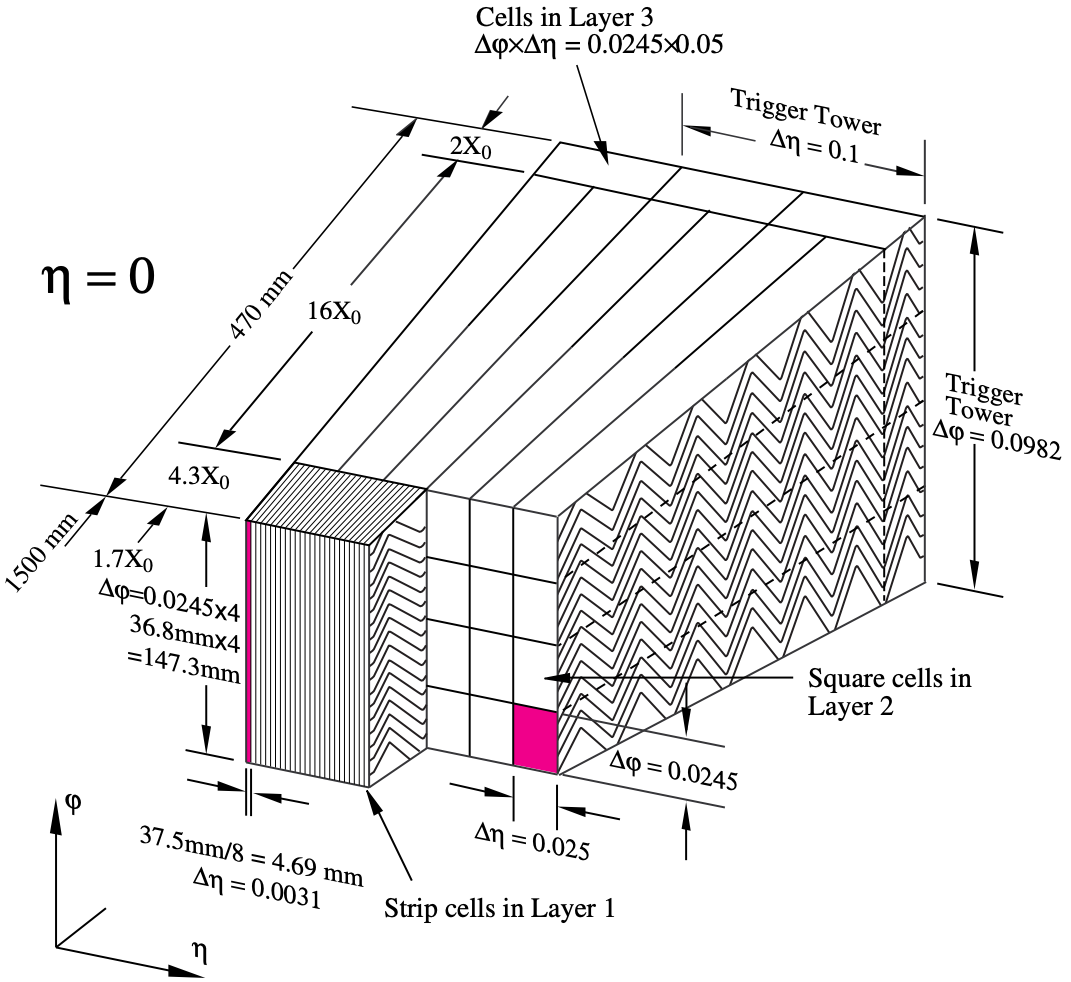
\includegraphics[width = 0.99\textwidth]{Chapter2/ATLAS_Calorimeters_ECAL}
	\caption{Sketch of section of the LAr EM barrel were the different layers are visible~\cite{ATLAS:2008xda}.}
    	\label{fig:Chap2:ATLAS:ECal}
  \end{subfigure}
  \hfill
  \begin{subfigure}[b]{0.49\textwidth}
    	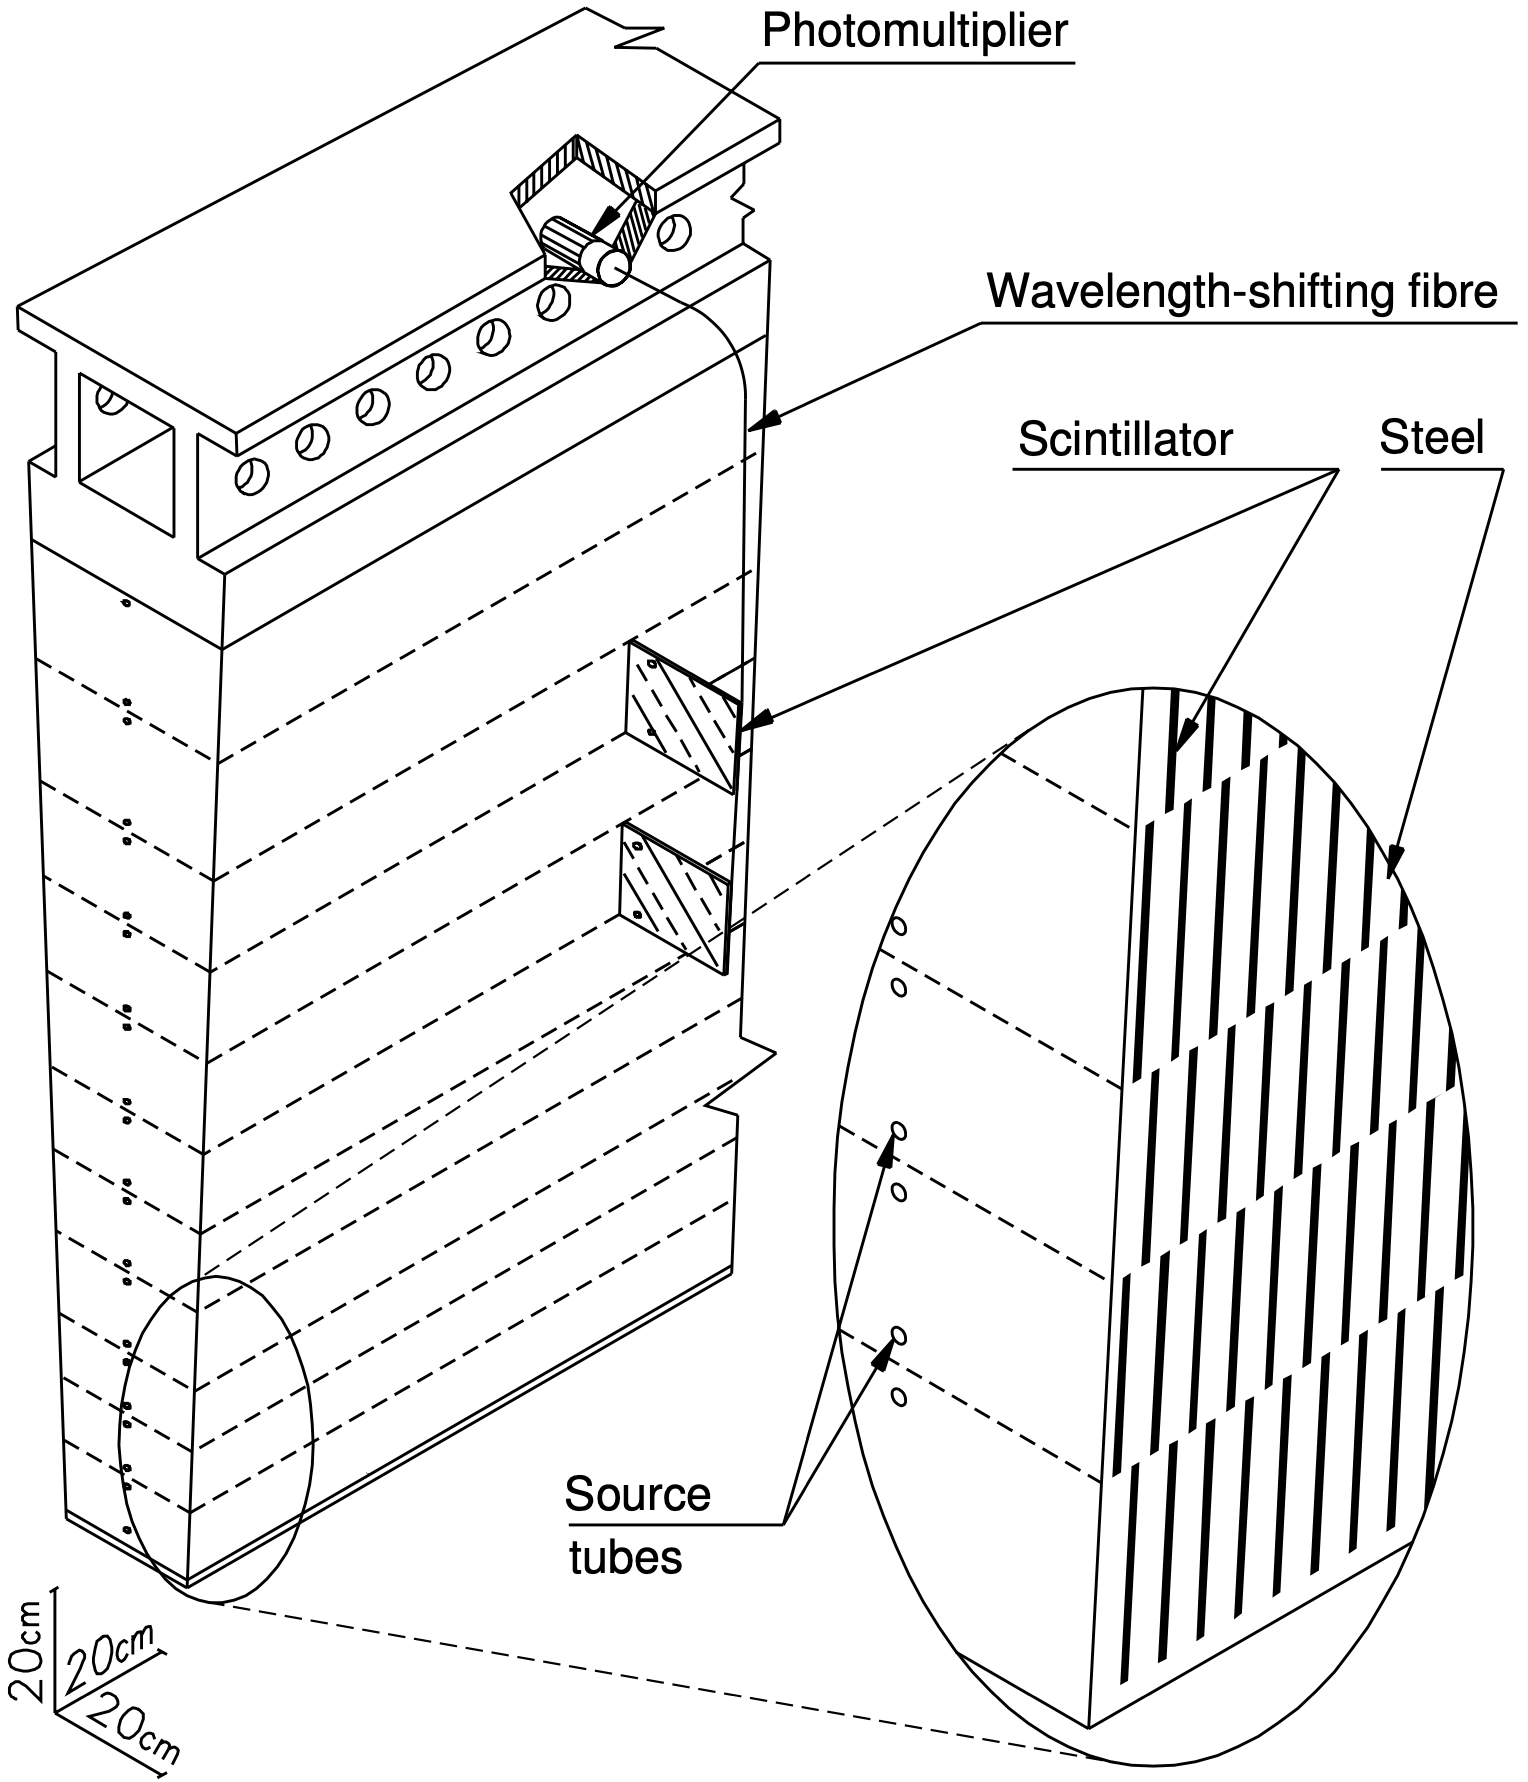
\includegraphics[width = 0.99\textwidth]{Chapter2/ATLAS_Calorimeters_HCAL}
	\caption{Mechanical assembly and optical readout of the tile calorimeter of the HCAL.}
    	\label{fig:Chap2:ATLAS:HCal}
  \end{subfigure}
  \caption{Sketch of a section of the ATLAS (a) ECAL and (b) HCAL~\cite{ATLAS:2008xda}.}
\end{figure}
\end{comment}



%%%%%%%%%%%%%%%%%%
%         Hadronic calorimeter        %
%%%%%%%%%%%%%%%%%%
\subsubsection{Hadronic calorimeter}
\label{sec:Chap2:CALO:HCAL}
The HCAL~\cite{Cavallari_2011} is made of a sampling calorimeter of steel and plastic 
scintillator tiles covering the pseudorapidity region of $|\eta|<1.7$ in the barrels. The end-caps 
are made of copper and LAr, covering $1.5<|\eta|<3.2$, and are embedded in the end-caps of the ECAL.
 This calorimeter uses 9800 electronic channels in the barrel and 5600 in the end-cap. With 2900 tones, the HCAL is the heaviest part
 of the ATLAS detector. It has 420000 scintillator tiles and 9500 photomultiplier tubes~\cite{ATLAS_Web_Detectors}.
 %All these elements are shown in Figure~\ref{fig:Chap2:ATLAS:HCal}, where the tiles, the fibres and the photomultipliers are visible.
 The scintillating-light signal produced at the tiles is read by photomultipliers tubes. 
 
 The contribution of the electronic noise is negligible for the tile calorimeter, therefore, its energy resolution only has
 the stochastic and constant terms~\cite{Cavallari_2011}:
 \begin{equation*}
	\frac{\sigma_E}{E}=  \frac{5.9\%}{\sqrt{E}} \oplus 5.7 \% \, .
\end{equation*}




%%%%%%%%%%%%%%%%%
%         Forward calorimeter        %
%%%%%%%%%%%%%%%%%
\subsubsection{Forward calorimeter}
In addition to the ECAL and HCAL, a smaller calorimeter is placed in the end-caps surrounding 
the beam pipe to cover the forward region ($3.1<|\eta|<4.9$), the forward calorimeter (FCAL). 
This coverage is required for many physics tasks such as the reconstruction of the 
missing transverse energy of the forward-jet tagging.

This calorimeter is a sampling calorimeter based on LAr as active medium and copper as absorber. 
The thickness of the FCAL is optimised to achieve high absorption, approximately, 10 radiation lengths~\cite{CERN-LHCC-96-041}. %~\cite{TarekAbouelfadlMohamed2020} $X_0$

This detector has a resolution of:
 \begin{equation*}
	\frac{\sigma_E}{E}=  \frac{100\%}{\sqrt{E}} \oplus 10 \% \,.
\end{equation*}



%%%%%%%%%%%%%%%
%       Muon Chambers        %
%%%%%%%%%%%%%%%
\subsection{Muon Spectrometer}
\label{sec:Chap2:ATLAS:MS}
%https://inspirehep.net/files/b9fa23188a4052f96dfc8d9e33454ec3
The muons can penetrate through calorimeters and reach the last layer of the ATLAS detector, the MS~\cite{ATLAS:1997ad}. %This system is responsable for muon measurements.
Figure~\ref{fig:Chap2:ATLAS:MS} shows a schematic cut-away view of the ATLAS MS.

\begin{figure}
\centering
\begin{minipage}{.64\textwidth}
 	\centering
 	 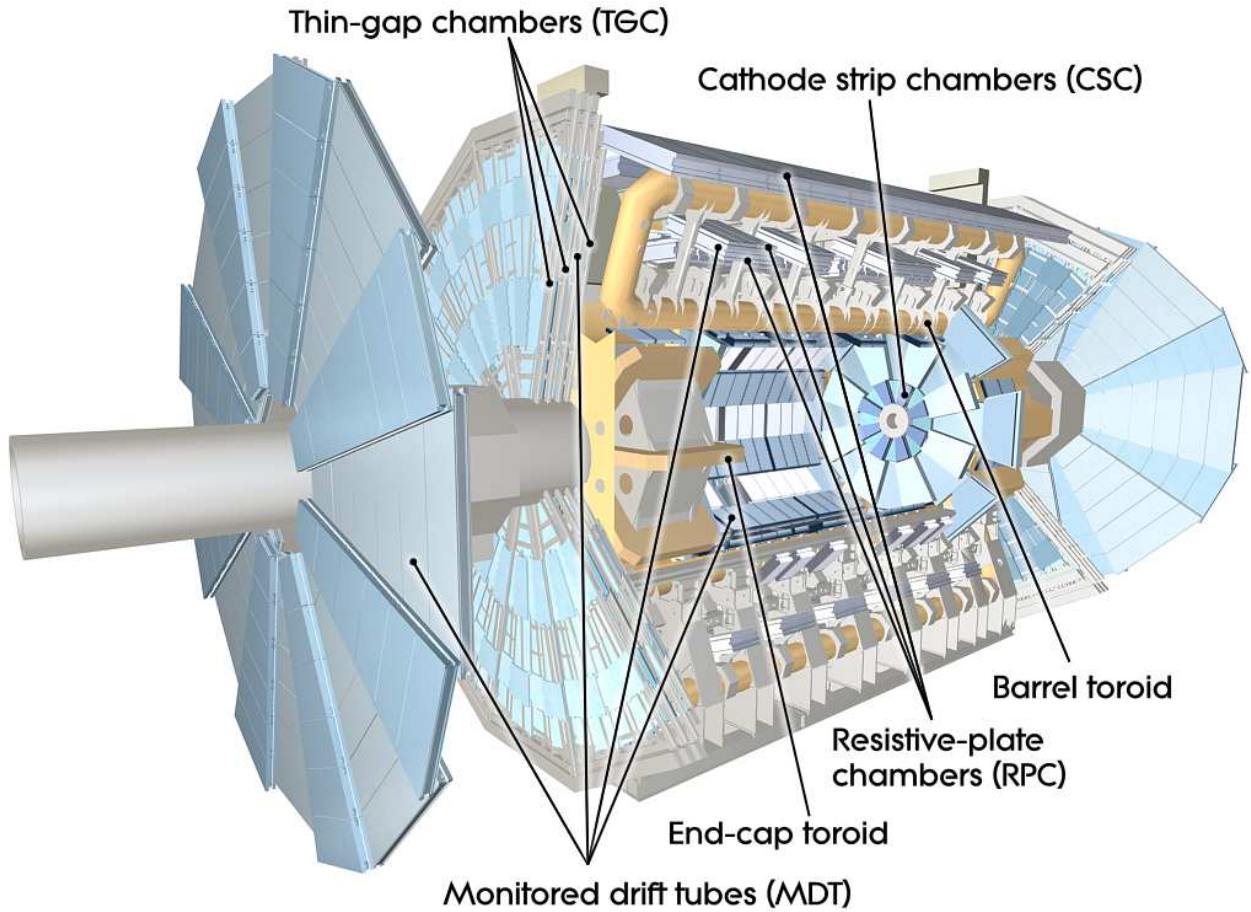
\includegraphics[width = 0.95\textwidth]{Chapter2/ATLAS_MuonSpectrometer}
	 \caption{Conceptual layout of the MS (blue). \\The magnet system (yellow) is also shown~\cite{ATLAS:2008xda}.}
	 \label{fig:Chap2:ATLAS:MS}
  \label{fig:test1}
\end{minipage}%
\begin{minipage}{.35\textwidth}
 	\centering
	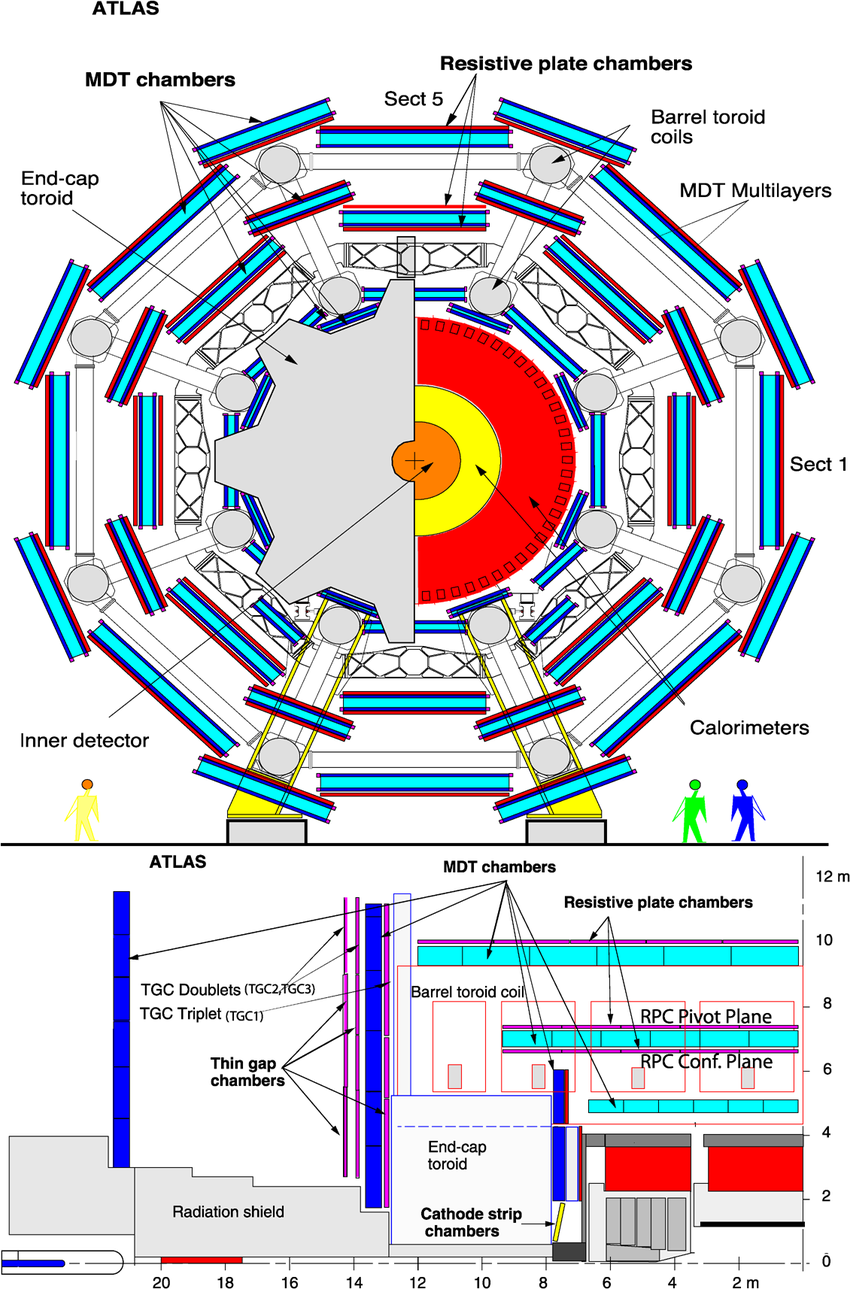
\includegraphics[width = 0.9\textwidth]{Chapter2/ATLAS_MuonSpectrometer_Scheme}
	\caption{ATLAS Muon detectors~\cite{ATLAS:1997ad}.} 
	\label{fig:Chap2:ATLAS:MS:Scheme}
\end{minipage}
\end{figure}


%\begin{figure}
% 	\centering
% 	 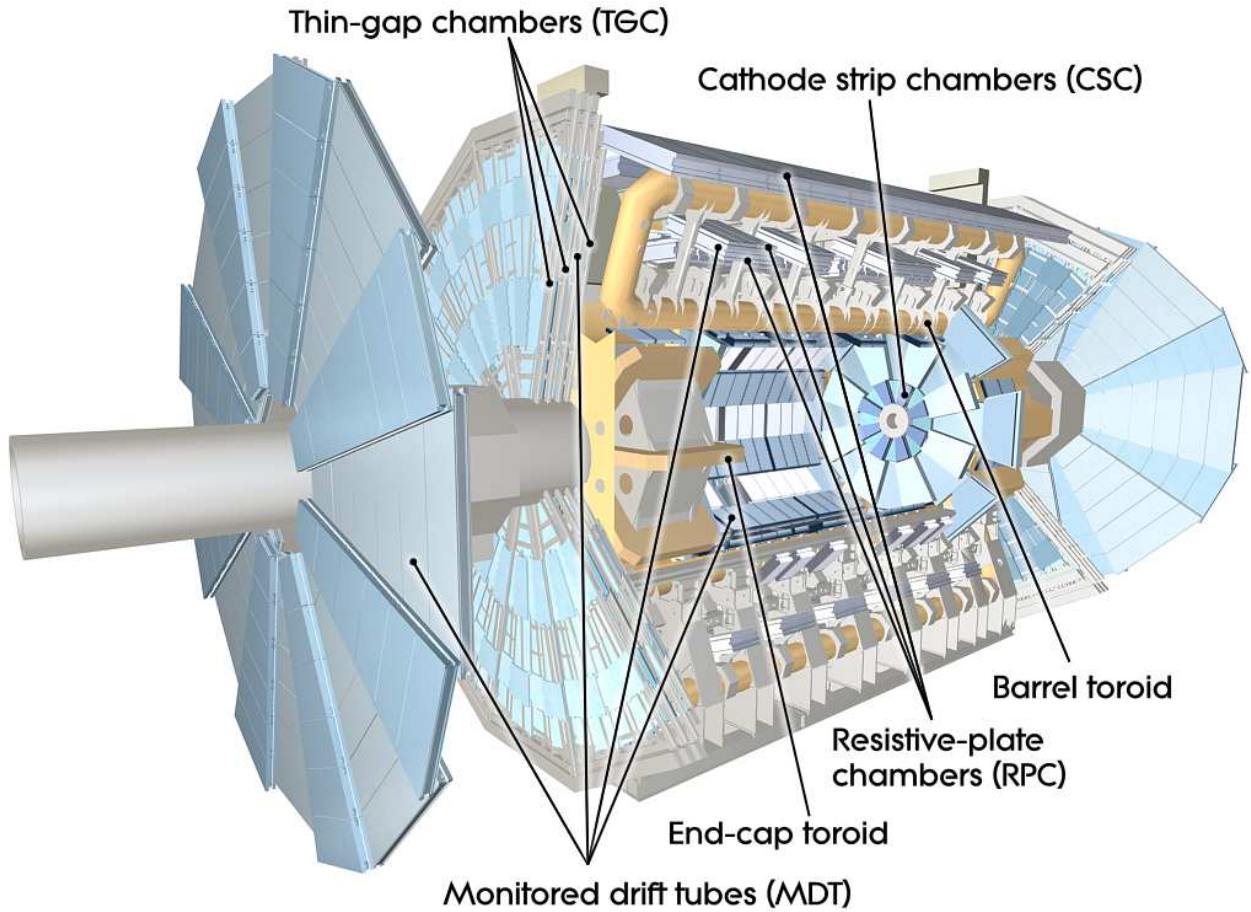
\includegraphics[width = 0.75\textwidth]{Chapter2/ATLAS_MuonSpectrometer}
%	 \caption{Conceptual layout of the MS (blue). The magnet system (yellow) is also shown~\cite{ATLAS:2008xda}.}
%	 \label{fig:Chap2:ATLAS:MS}
%\end{figure}

%\begin{wrapfigure}{r}{0.4\textwidth}
%	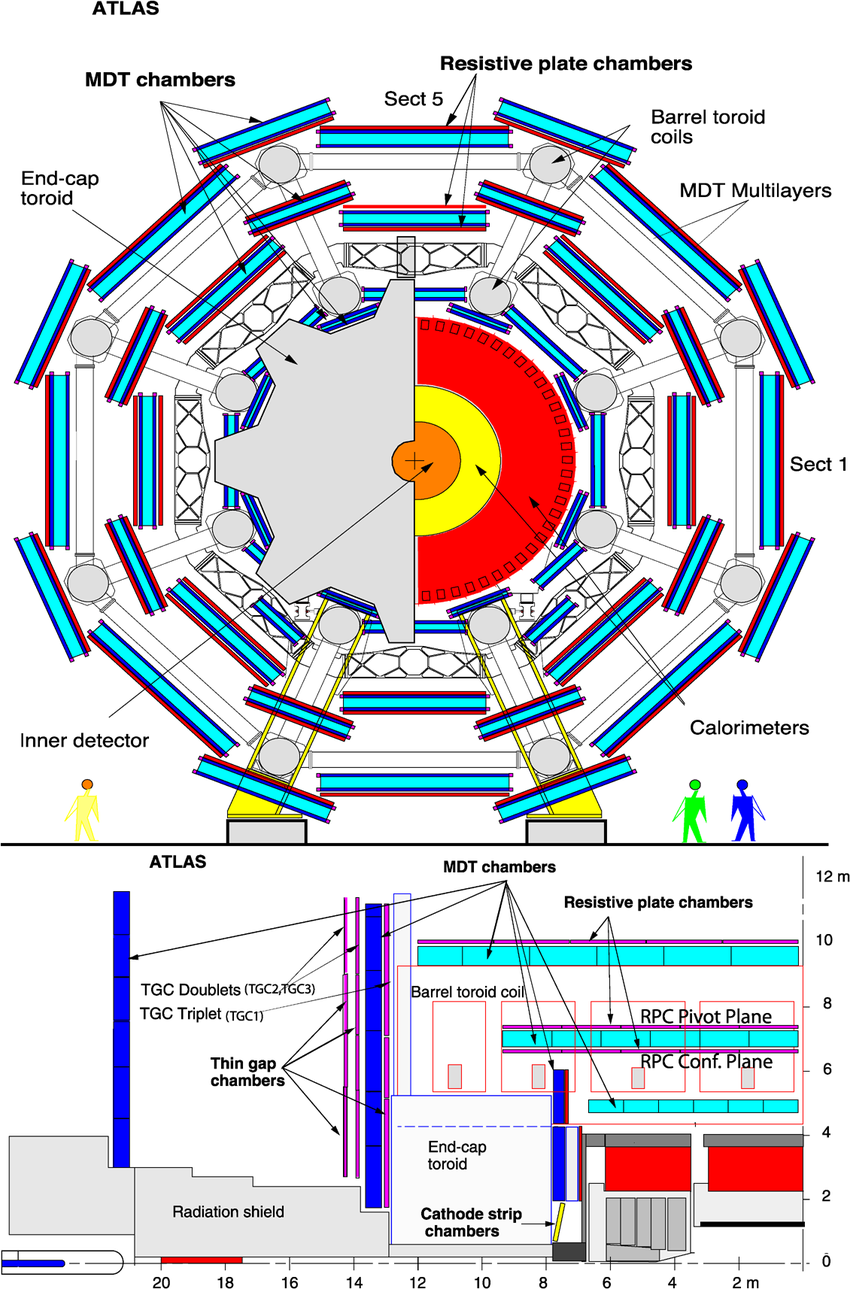
\includegraphics[width = 0.4\textwidth]{Chapter2/ATLAS_MuonSpectrometer_Scheme}
%	\caption{ATLAS Muon detectors.} 
%	\label{fig:Chap2:ATLAS:MS:Scheme}
%\end{wrapfigure} 

% Magnet system of the MS
The MS surrounds the calorimeters and it aims to measure the trajectories of muons 
%to determine their direction and momentum with excellent tracking precision
%as well as their electric charge in 
with a pseudorapidity coverage of $|\eta| < 2.7$.  %The MS
%is also an essential component of the ATLAS trigger system,
%which decides in real-time which events to record for further analysis.
%To bend the particle tracks after they exit the HCAL, the MS uses eight large 
%superconducting air-core toroid magnets in $|\eta| < 1.4$ region.
%For the $1.6 < |\eta| < 2.7$, the tracks are bent by magnets inserted in the end-caps. 
%In the transition region, $1.4 < |\eta| < 1.6$, the magnetic field responsible for bending
%the particles is provided by both the air-core toroid magnets and the smaller end-cap magnets. 
%These fields are perpendicular to the trajectory of the muons originated in the IP. More details 
%about the magnet systems of the MS can be found in Section~\ref{sec:Chap2:MagnetSystem}.


% Sub-detectors of the MS
The MS instrumentation is based, on the one hand, on precision chambers for the coordinate measurements in the bending plane: 
Monitored Drift Tube chambers (MDT) and Cathode-Strip Chambers (CSC), and, on the other hand, on trigger chambers:
Resistive Plate Chambers (RPC) and Thin Gap Chambers (TGC).  Table~\ref{tab:Chap2:ATLAS:MS} gives a summary of the MS 
detector components.  %In Figure~\ref{fig:Chap2:ATLAS:MS:Scheme} the distribution of the MS detectors is described.

%The four MS detector components are summarised in
%Table~\ref{tab:Chap2:ATLAS:MS} and its distribution in described in Figure~\ref{fig:Chap2:ATLAS:MS:Scheme}.

\begin{table}[h]
\centering
\begin{tabular}{llll}
\toprule
Type & Purpose  & Location         	& Coverage 			\\ \midrule
MDT  & Tracking & Barrel + end-cap &  $0.0 < |\eta| < 2.0$       	\\
CSC  & Tracking & End-cap layer 1  	&  $2.0 < |\eta| < 2.7$       	\\
RPC  & Trigger    & Barrel           	&  $0.0 < |\eta| < 1.0$     	\\
TGC  & Trigger    & End-cap          	&  $1.0 < |\eta| < 2.4$        \\
 \bottomrule
\end{tabular}
\caption{Summary ATLAS MS subdetectors~\cite{Ishii:2001hy}.}
\label{tab:Chap2:ATLAS:MS}
\end{table}
%The precision in momentum resolution is about $10 \%$ for 1 TeV tracks. 

\begin{itemize}
	\item \textbf{Monitored Drift Tube chambers}~\cite{Livan:319197}: 
		The MDT chambers provide precise momentum
		measurements covering $|\eta|<2.7$. 
		They determine %with high accuracy 
		the curve of the tracks. %This part of the MS cover a 
		%pseudorapidity range of $|\eta| < 2.7$. 
		The MDTs are designed to 
		have stand-alone measurement capability to 
		safeguard against any unanticipated background and to ensure 
		good discovery potential in the scenario of unexpected topologies. 
		To do so, the MDT uses a system of high-pressure (3 bar) drift tubes.
		%In the barrel region, the MDTs are arranged in three cylindrical stations 
		%coaxial to the beam axis and in the end-cal, the MDTs are vertically installed in three layers. 
		%An MDT chamber  consists of six laters of drift tubes (as depicted in Figure 
		%\ref{fig:Chap2:ATLAS:MS:MDT}), each of them with $3\,$cm of diameter, filled with gas. 
		%A tube can achieve a single wire resolution of $80\,$\textmu m~\cite{Ishii:2001hy}.
		An MDT chamber  consists of six laters of drift tubes, each of them with $3\,$cm of diameter, filled with gas. 
		A tube can achieve a single wire resolution of $80\,$\textmu m.
		In the entire MDT system, there are $1\,171$ chambers with a total of $354\,240$ tubes.
		
		%\begin{figure}[h]
 		%  \centering
  		%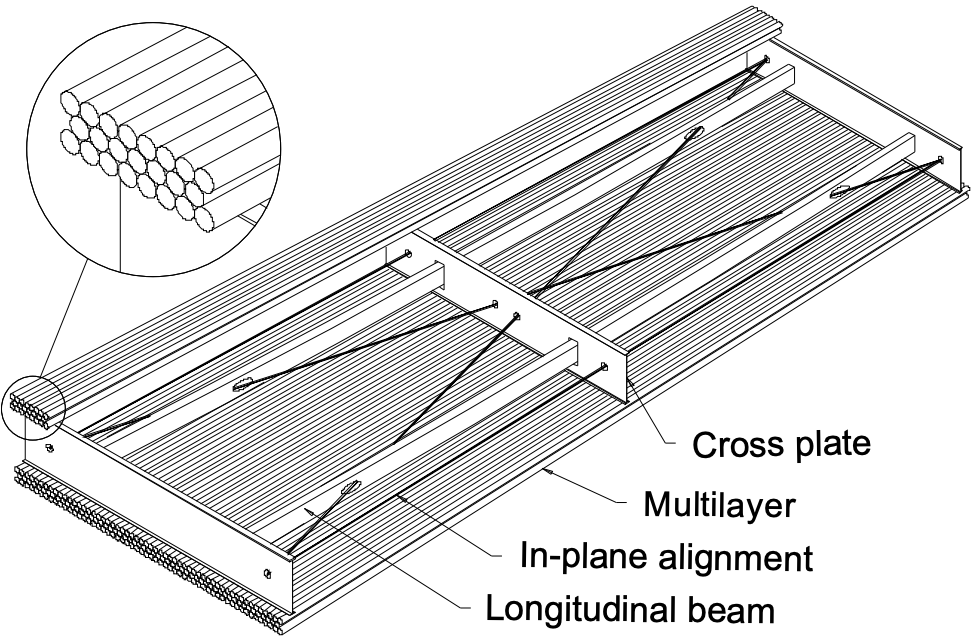
\includegraphics[width=.4\linewidth]{Chapter2/ATLAS_MuonSpectrometer_MDT}
  		%\caption{Schematic view of an MDT chamber.}
  		%\label{fig:Chap2:ATLAS:MS:MDT}
		%\end{figure}

	\item \textbf{Cathode-Strip Chambers}: It is the innermost tracking layer of the MS. 
		The CSCs are multi-wire proportional chambers filled of a mixture of gases with cathode strip read-out.
		Due to its higher rate capability and time resolution, it is located close to the beam 
		axis, where the particle fluxes are higher. 
		They have a higher granularity than the MDT.
		This component of the MS
		covers the range $2.0 < |\eta| < 2.7$. It measures with precision the coordinates 
		at the ends of the detector. It has $70\,000$ electric channels and provides a resolution of 
		around $60\,$\textmu m. 
		
	\item \textbf{Resistive Plate Chambers}~\cite{Cattani_2011}: This is the barrel element of the trigger system. 
		These chambers are located on both sides of the central CSC and inside the outermost CSC station, covering
		the $|\eta| < 1.0$ range.
		The RPCs are gaseous detectors used for triggering and for measuring the second coordinate in the barrel region.
		RCPs provide a time-space resolution of $1 \, \textrm{cm} \, \times  1\,\textrm{ns}$.
		The gas gap is of the order of $2\,$mm and the plate external surfaces are coated by thin layers of graphite 
		painting that allows uniform distribution of the high voltage along the plates.
		This part of the MS  is composed of $3\,800$ electric channels.
		
	\item \textbf{Thin Gap Chambers}~\cite{Nagai:1996mf}: 
		The TGCs are multi-wire proportional chambers filled with a mixture of gases with a
		smaller distance between cathodes and the wire plane compared to the distance between wires.
		As a first-level trigger, they have to 
		provide high efficiency and excellent time resolution for bunch-crossing tagging in a 
		high-background environment. The TGC presents a $2.0 < |\eta| < 2.7$  
		coverage. The particle flux received by the TCG is higher than that of the RPC.
		The three TGCs are located near the middle end-cap MDT station, in the forward regions.
		The intrinsic spatial resolution for a single layer is $45\,$\textmu m for a perpendicular incident angle, 
		and the transition region between pads is measured to be about $4\,$mm.
		TGCs measure the second coordinate in the non-bending direction with their circa $440\,000$ electrical channels.
\end{itemize}
 
%\begin{figure}
%\centering
%\begin{minipage}{.45\textwidth}
%  \centering
%  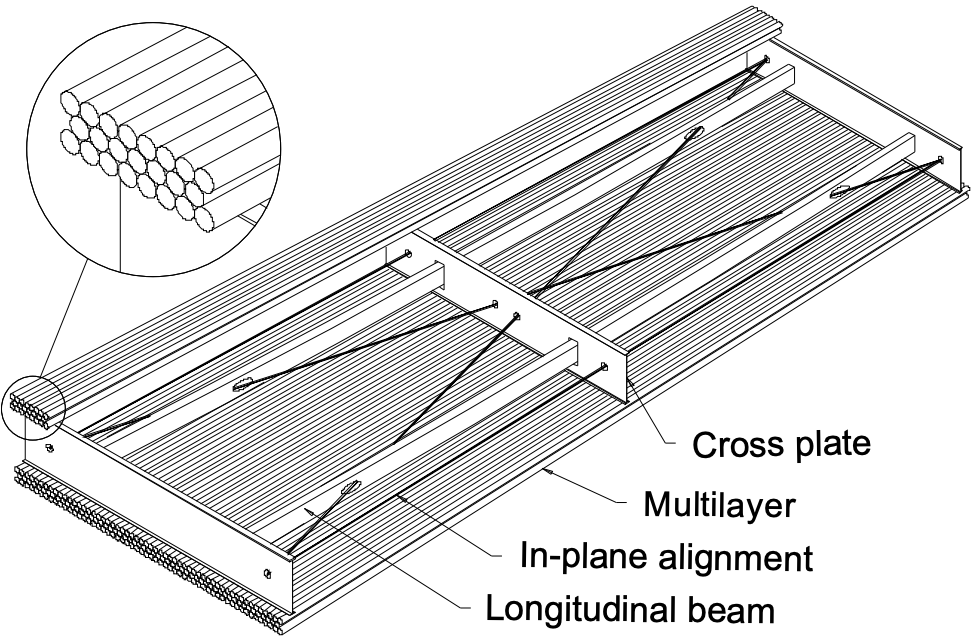
\includegraphics[width=.99\linewidth]{Chapter2/ATLAS_MuonSpectrometer_MDT}
% \captionof{figure}{Schematic view of an MDT chamber.}
%  \label{fig:Chap2:ATLAS:MS:MDT}
%\end{minipage}%
%\begin{minipage}{.54\textwidth}
 % \centering
 % 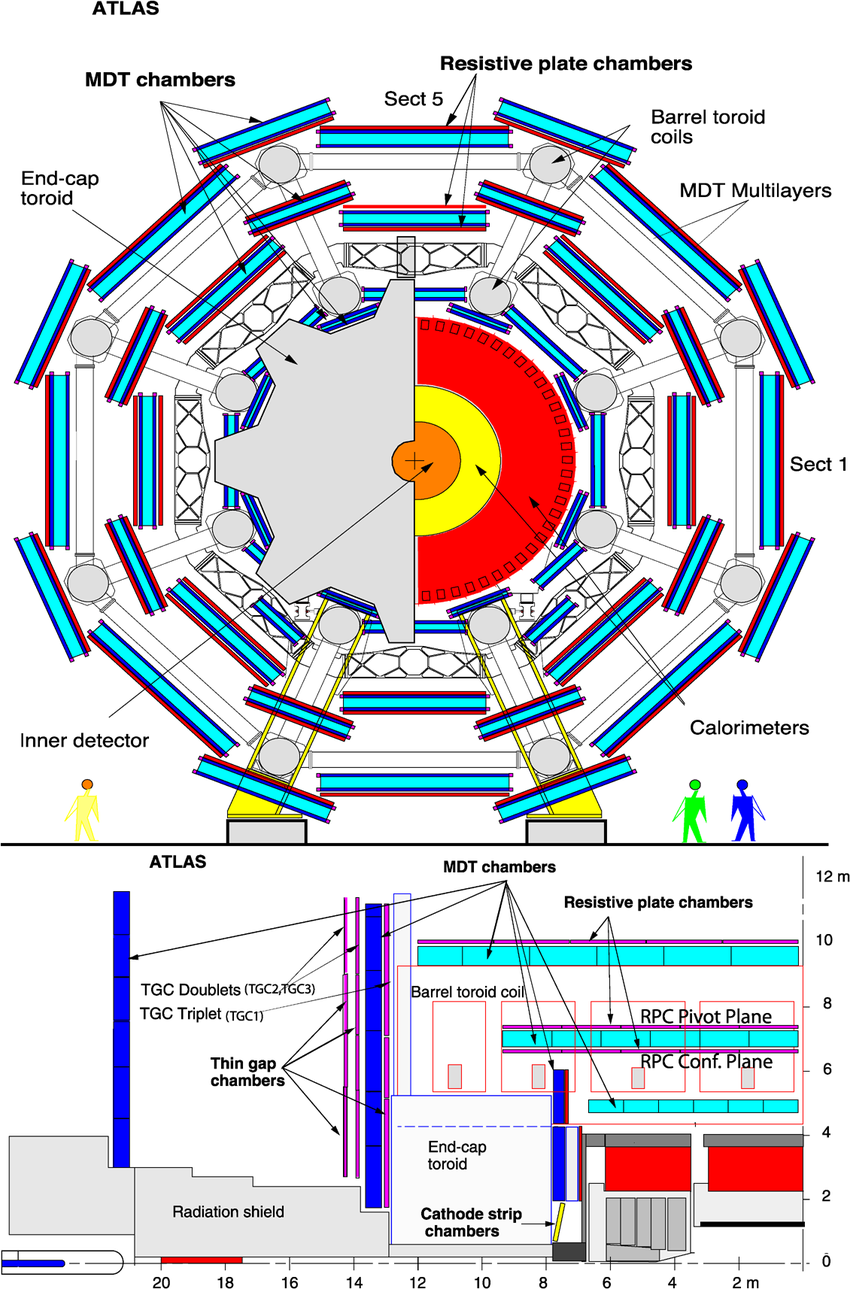
\includegraphics[width=.99\linewidth]{Chapter2/ATLAS_MuonSpectrometer_Scheme}
 % \captionof{figure}{ATLAS muon detectors.}
 % \label{fig:Chap2:ATLAS:MS:Scheme}
%\end{minipage}
%\end{figure}



%%%%%%%%%%%%%%%
%         Magnet system        %
%%%%%%%%%%%%%%%
\subsection{Magnet system}
\label{sec:Chap2:MagnetSystem}
\begin{comment}
%The ATLAS Barrel Toroid is the world's largest superconducting magnet. It works along the two end-cap Toroids and a 
%central eight Solenoid magnet to bend the paths of charged particles produced at collisions in the LHC. 
 
The curvature of the tracks of the particles is fundamental to measure the transverse momentum and the charge of the particles.
To bend the path of charged particles, these are immersed in a homogeneous magnetic field which is produced by the 
both the toroidal and solenoid magnets.
The bending power of a charged particle in a magnetic field is determined by  $\int B dl$, 
where $B$ represents the component of the magnetic field that is orthogonal to the direction 
of the motion of the charged particle.

ATLAS magnetic system is divided into three subsystems: the central solenoid magnet, the barrel toroids (BT) and the end-cap toroid (ECT).

% Central solenoid magnet
\subsubsection{Central solenoid magnet}
The ATLAS solenoid surrounds the ID  providing a $2\,$T magnetic at the centre of the tracking volume. 
This magnet is very thin, having only $4.5\,$cm thickness, which 
minimises the interaction of the particles with the magnet material. It is important to not use a lot 
of material here because, otherwise, the interaction of the particles with
the solenoid magnet would impact negatively in the performance of the calorimeters.
To achieve such a field within a small thickness, $9\,$km of NbTi superconductor wires 
into strengthened, pure aluminium strips  and cooled down to $4.5\,$K are used.
The central solenoid magnet has a cylindrical shape with a diameter of $5.6\,$m and a length of $2.56\,$m, and it weights $5\,$tonnes.

% Toroid magnets
\subsubsection{Toroid magnets}
Three large air-core toroids (one barrel and two end-caps) generate the magnetic field in the MS. %The
%magnetic field provided by the toroid magnets is $3.5\,$T. 
Each toroid consists of eight coils assembled with cylindrical symmetry (see the yellow elements in Figure~\ref{fig:Chap2:ATLAS:MS}).
The coils are based on an aluminium stabilised NbTi alloy (Al/NbTi/Cu) superconductor operating
at $4.5\,$K~\cite{CERN-LHCC-97-018}.% The main difference between the barrel and end-cap toroids for the cold mass is that the latter has a higher critical
%current and less aluminium than the former~\cite{CERN-LHCC-97-018}.


\paragraph{Barrel Toroid} \mbox{}\\
The Barrel Toroid magnet is the largest component of the ATLAS magnet system.  It generates a toroidal magnetic field which,
as introduced in Section~\ref{sec:Chap2:ATLAS:MS},  is almost completely perpendicular to the track of the particles. 
In order to minimise the impact (i.e. reduce any interaction apart from applying magnetic field) of the magnet system with the particles, 
the barrel toroid is designed as an open and light structure.
The barrel toroid coils are housed in eight individual cryostats, with the linking elements
between them providing the overall mechanical stability. A view of the coils of the barrel toroid in their cryostats is in Figure~\ref{fig:Chap2:ATLAS:Magnet:BarrelToroid}.

%\begin{figure}
%	\centering
%	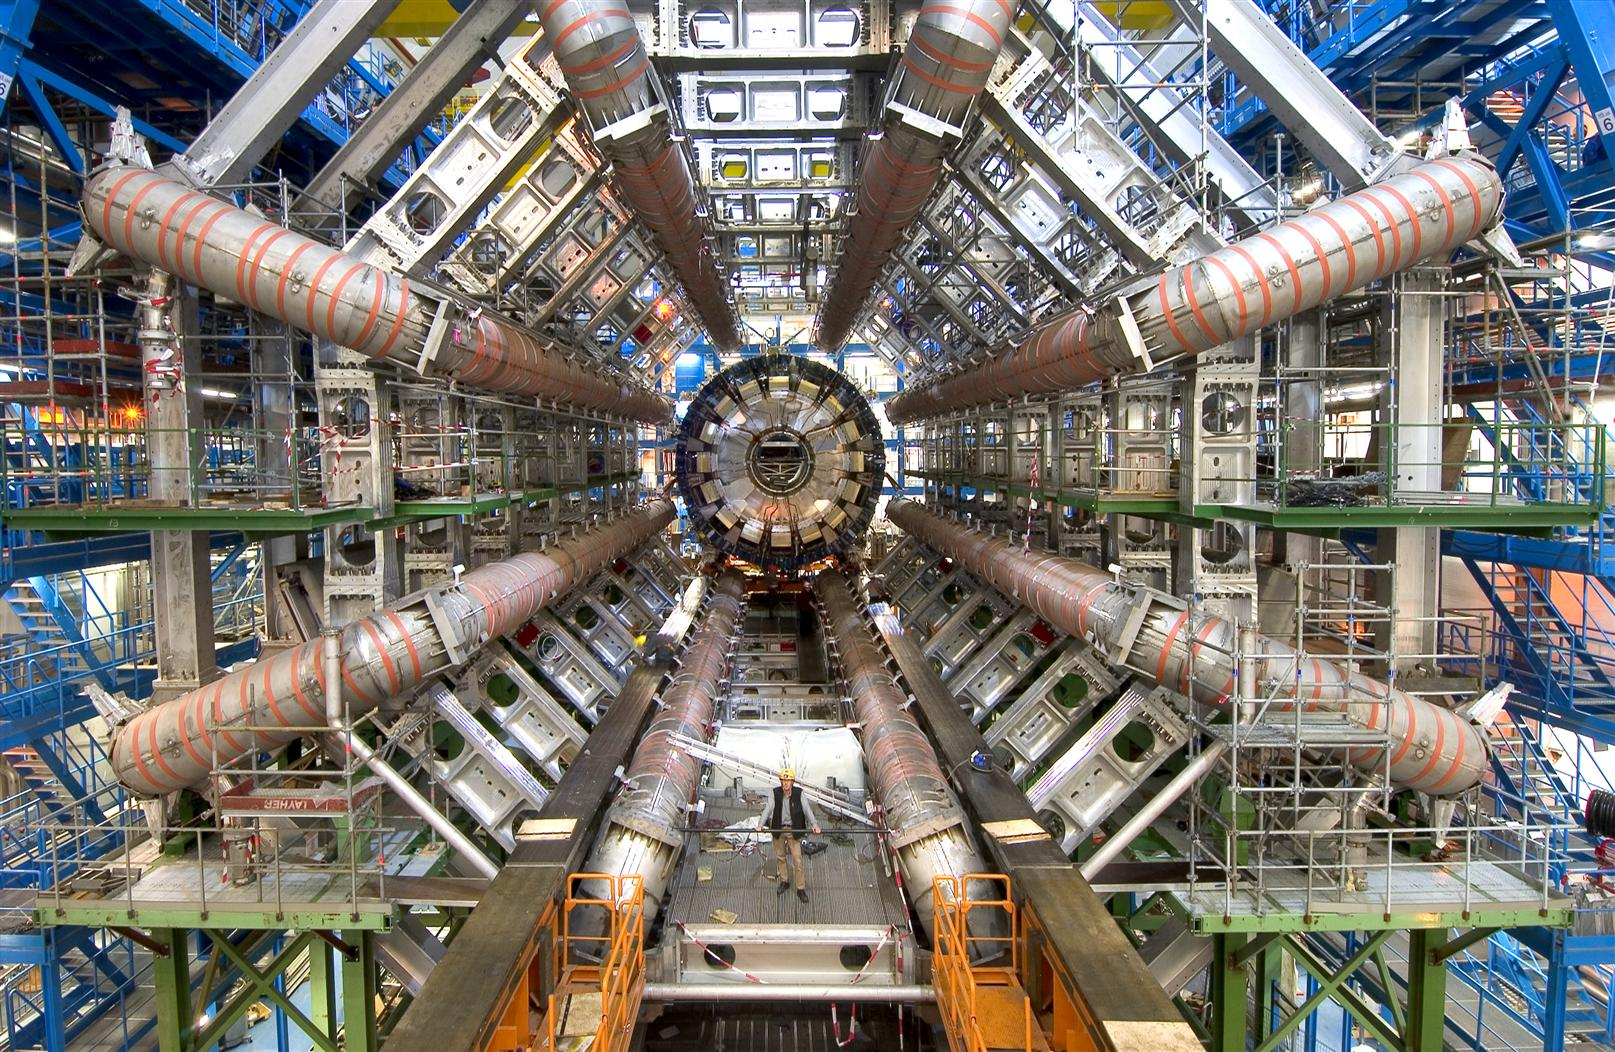
\includegraphics[width = 0.7\textwidth]{Chapter2/ATLAS_Magnets_BarrelToroid}
%	\caption{Picture of the installation ATLAS calorimeters. The eight coils that compose the ATLAS barrel toroid magnets are already installed in the cryostats.
%	Thus view is one of the most iconic of the ATLAS detector.}
%	\label{fig:Chap2:ATLAS:Magnet:BarrelToroid}
%\end{figure}

The magnetic flux density delivered by this magnet is $3.9\,$T on the superconductor.
For the toroid barrel, the bending power ($\int B dl$) is in the interval $1.5\,$Tm to $5.5\,$Tm in $0 <|\eta| <1.4$.
It is the largest toroidal magnet ever built ($25.3\,$m in length), being probably the most iconic and characteristic element of ATLAS. It
weights 830 tonnes and uses more than $56\,$km of superconducting wire~\cite{CERN-LHCC-97-018, ATLAS_Web_Detectors}.

\paragraph{End-cap Toroid} \mbox{}\\
The end-caps extend the magnetic field of the barrel toroid to the beam pipe. These magnets are constrained by the 
inner radius of the barrel toroid and the axial length of the experiment.
 
As well as in the barrel toroid, it has a $4.1\,$T magnetic field on the superconductor.
 For the end-cap toroid, the $\int B dl \in [4,\, 8]\,$ Tm in the pseudorapidity range $1.6 <|\eta| < 2.7$~\cite{CERN-LHCC-97-018}.
 In the transition region where the end-cap and barrel toroids overlap ($1.4 <|\eta| <1.6$), the bending power is lower.
 Each end-cap magnet (Figure~\ref{fig:Chap2:ATLAS:Magnet:EndCapToroid}) has a diameter $10.7\;$m and weights $240\,$tonnes~\cite{CERN-LHCC-97-018, ATLAS_Web_Detectors}.
 \begin{figure}
	\centering
	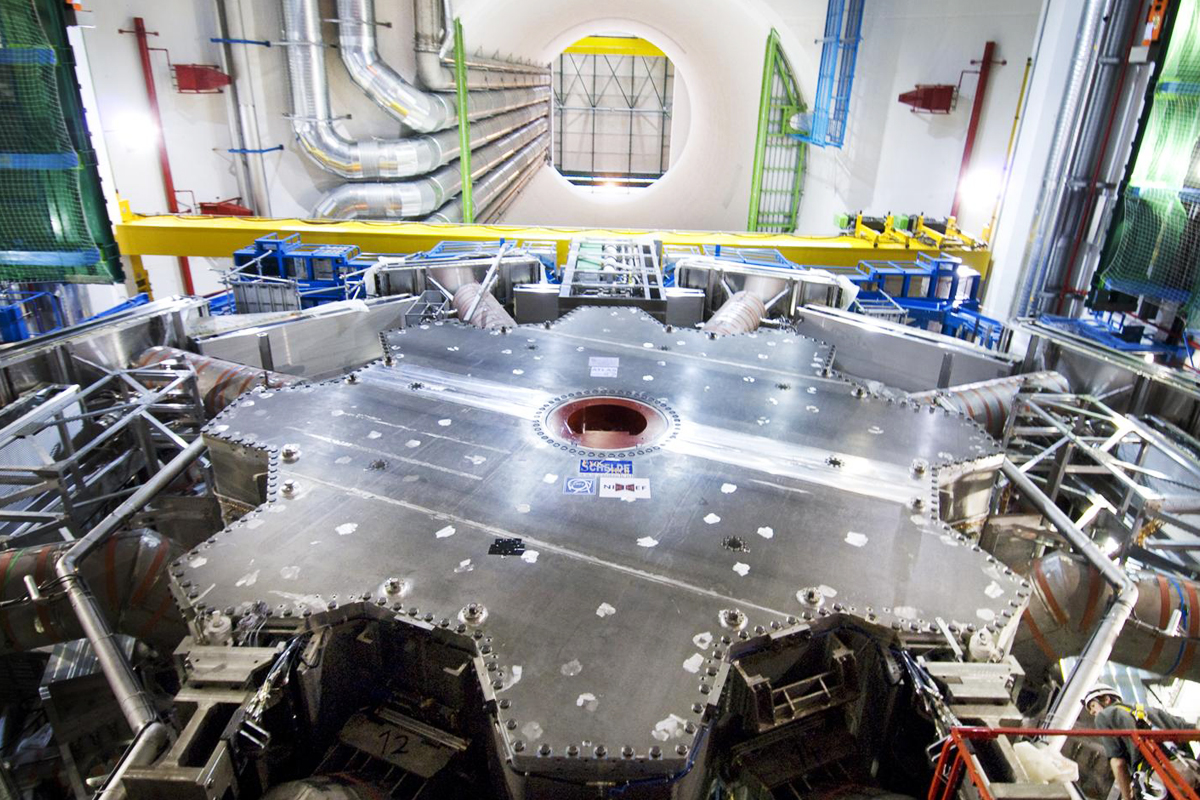
\includegraphics[width = 0.6\textwidth]{Chapter2/ATLAS_Magnets_EndCap}
	\caption{One of the two end-cap toroidal magnets. Each is made by eight superconducting coils with a magnetic field peaking at $4.1\,$T.}
	\label{fig:Chap2:ATLAS:Magnet:EndCapToroid}
\end{figure}
\end{comment}

%%
% Rewrite magnet section but shorter
%%
The curvature of particle tracks is crucial to determine their transverse momentum and charge. 
This bending is achieved through a homogeneous magnetic field produced by toroidal and solenoid 
magnets, with bending power proportional to $\int B dl$, where $B$ is the magnetic field component 
orthogonal to the charged-particle direction.

The ATLAS magnet system consists of three subsystems: the central solenoid, 
barrel toroids (BT), and end-cap toroid (ECT).

\begin{itemize}
	\item \textbf{Central solenoid magnet}: Surrounding the ID, the ATLAS solenoid provides 
	a $2\,$T magnetic field at the centre of the tracking volume. With a mere $4.5\,$cm thickness, 
	the particle interaction with the magnet material is minimised, ensuring optimal calorimeter performance. 
	This thin design leverages $9\,$km of NbTi superconductor wires in pure aluminium strips, 
	cooled to $4.5\,$K. The magnet has a cylindrical shape, $5.6\,$m in diameter and $2.56\,$m 
	in length, weighing $5\,$tonnes.
	
	\item \textbf{Barrel toroid magnets}: The BT, being the largest component of the magnet system, 
	generates a field almost perpendicular to particle tracks. Designed as a light and open structure 
	to minimise interference with particles, its coils are placed in individual cryostats linked for stability.
	This magnet offers a magnetic flux density of $3.9\,$T on its superconductor. As the largest of its kind, 
	it measures $25.3\,$m in length, weighs 830$\,$tonnes, and utilises over $56\,$km of superconducting 
	wire~\cite{CERN-LHCC-97-018, ATLAS_Web_Detectors}.
	These air-core toroids of the toroid magnets use an Al/NbTi/Cu superconductor operating at 
	$4.5\,$K~\cite{CERN-LHCC-97-018}.

	\item \textbf{End-cap toroid magnets}: Extending the magnetic field of the BT, the ECTs ensure uniform 
	coverage. Their $4.1\,$T magnetic field on the superconductor has bending power between $4\,$ and 
	$8\,$Tm in the range $1.6 <|\eta| < 2.7$~\cite{CERN-LHCC-97-018}. Each ECT, with a diameter of $10.7\;$m 
	and weighing $240\,$tonnes, overlaps with barrel toroids in the range $1.4 <|\eta| <1.6$, where
	bending power is reduced.
\end{itemize}

%\pablo{- Conseguir imagen vectorial del Magnet System -}


%%%%%%%%%%%%%%%%
%         Trigger and DAQ         %   TDAQ
%%%%%%%%%%%%%%%%
\subsection{Trigger and Data Acquisition System}
\label{sec:Chap2:Trigger_and_DAQ}
The proton bunches cross at the centre of the ATLAS detector $40\,$M times per second, resulting in approximately 
(assuming Run 2 mean pile-up\footnote{The pile-up refers to the simultaneous occurrence of multiple $\Pproton \Pproton$ 
collisions in a single bunch crossing, leading to an overlap of signals. It is described with
more detail in Section~\ref{sec:Chap2:LHC:pileup}.} <$\mu$>$=33.7$)
 $1\,200\,$million $\Pproton \Pproton$ collisions per second. 
 %Even though the bunches are composed by $\sim 10^{11}\,$, there are only around $30\,$collisions per crossing with nominal beam currents.
Reading out and storing all the information from these interactions is not feasible since it has a combined data volume of more than 60 million MB per second.
Only some of these events are of interest to physics studies and, consequently, only this subset needs to be saved into permanent storage for later analysis.
To select only interesting data, ATLAS uses a complex and highly distributed Trigger and Data Acquisition System (TDAQ) 
\cite{ATLAS:2003aa} that reduces the rate of 
recorded data from the initial $40\,$MHz to just an average of $1\,$kHz. The reduction through the trigger is carried in two steps: 
The custom-built electronic performs an initial selection and, afterwards, a software-based system analyses the data that passes the initial filter. 


%The TDAQ system is an essential component of ATLAS in charge of processing the events online, selecting the relevant ones and storying them.
%To do so, the TDAQ verifies for each bunch crossing if at least one among the hundred conditions is satisfied. 
%These conditions, also known as ``triggers'', are based on identifying both combinations of candidate physics objects (``signatures'') % Physics objects such as: electrons, photons muons, jets, jets with b-flavour tagging
%and global properties of the events~\cite{ATLAS:2012nks}. % Global event properties such as MET or HT
%Figure~\ref{fig:Chap2:ATLAS:Trigger} shows a diagram of the TDAQ system, in this figure can be seen the different components 
%as well as the detector read-out and data flow.

 %\begin{figure}
%	\centering
%	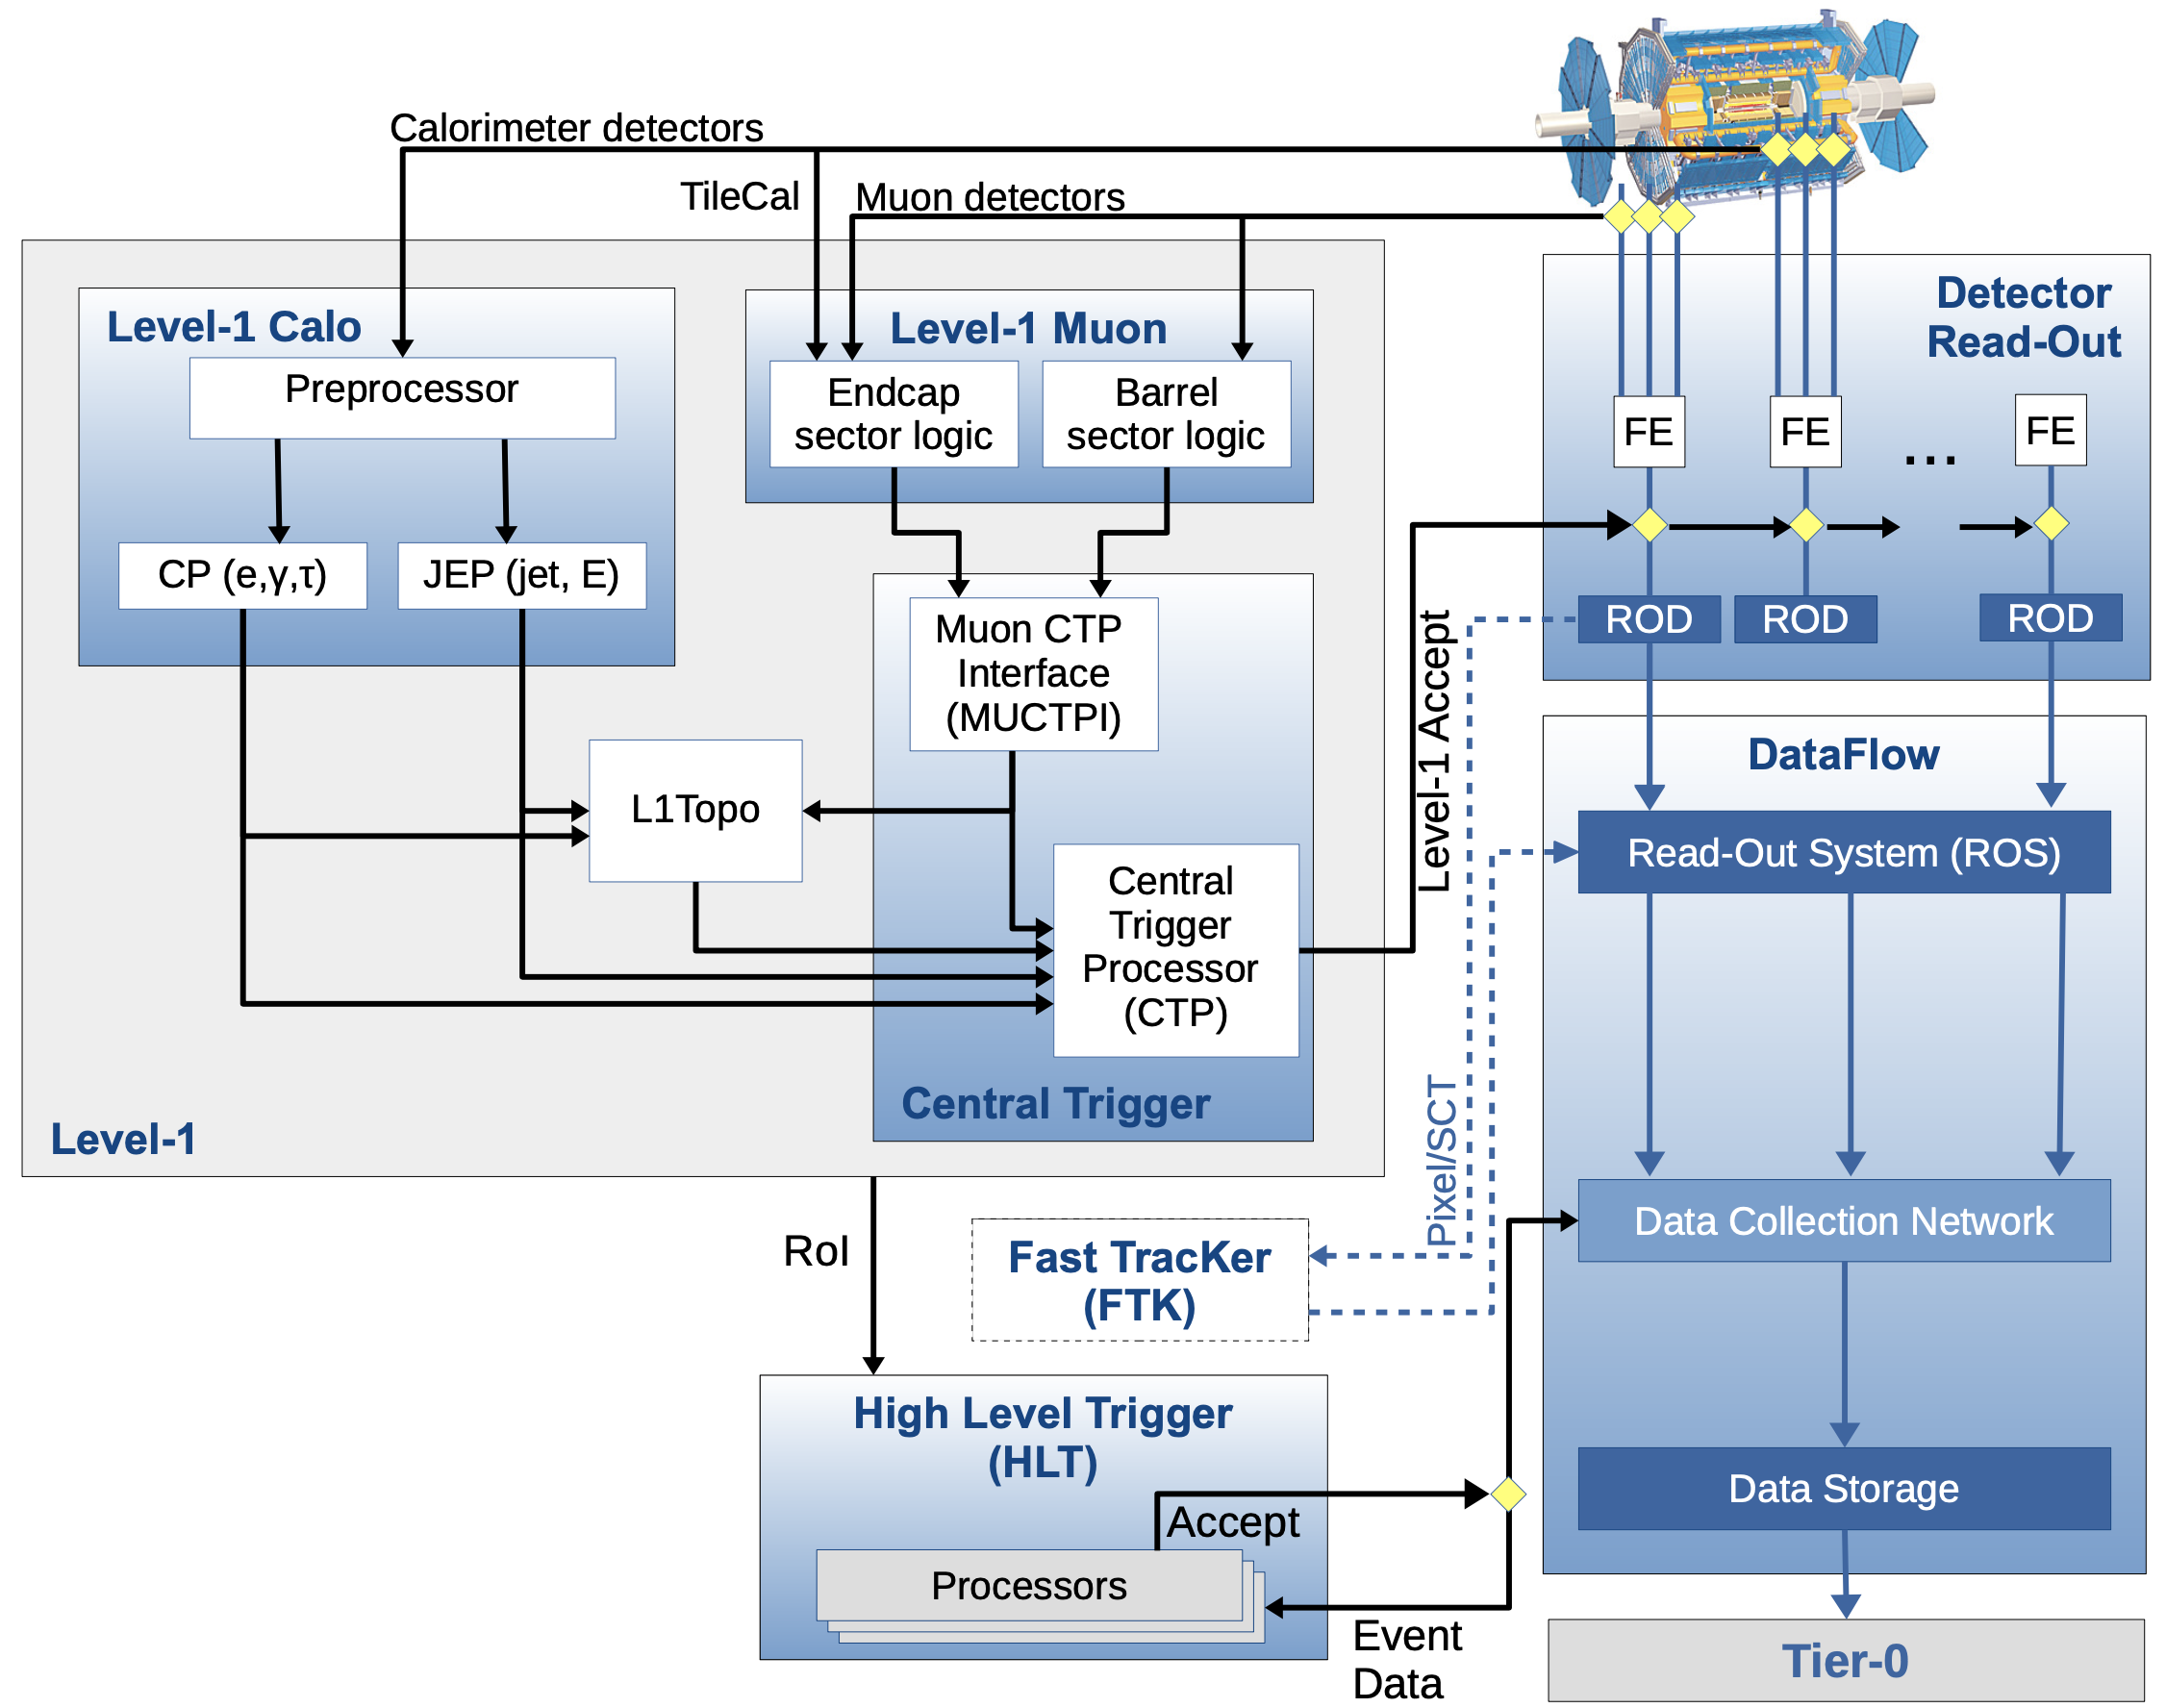
\includegraphics[width = 0.85\textwidth]{Chapter2/ATLAS-Trigger}
%	\caption{The ATLAS TDAQ system in Run 2.}
%	\label{fig:Chap2:ATLAS:Trigger}
%\end{figure}


%\subsubsection{Level 1 Trigger}
The first-level trigger (L1) is a hardware-based filter. %performed by ATLAS sub-detectors. 
The L1 uses the information of the partial granularity of the Calorimeters and the MS %(but not the ID)
to select events up to the maximum-readout rate of the detector ($100\,$kHz) within a latency of $2.5\,$\textmu s. 
% number from https://cds.cern.ch/record/2016651/files/ATL-DAQ-PROC-2015-018.pdf
% L1 can filter events ase in:
%	Event-level quantities: the total energyin the calorimeter)
%	Multiplicity of objects above thresholds: the transverse momentum of a muon, etc.
%	Topological requirements: invariant masses or angular distances)
Additionally, the L1 identify the regions of interest (RoI), which includes the position and the \pT of the candidate objects.

%For each event accepted by the L1, the Front-End (FE) detector electronics read the detectors data and pass it to the ReadOut Drivers (ROD).
%The ROD performs the initial processing and formatting and the ReadOut Systems (ROS) buffers  this data. 

%\subsubsection{High Level Trigger}
The data from filtered from the L1 is sent to the software-based trigger, 
the so called ``High Level Trigger'' (HLT)~\cite{ATLAS:2003aa}. %, when is requested by the HLT.
This software-based system is executed on a farm of computers, % (using about $40\,000$ CPU cores). 
making use of fast-trigger algorithms. %, it provides early rejection that are followed by more precise
%algorithms that relay on Athena.

An average $1.2\,$kHz output rare for Run 2 passes the HLT (with a latency of just 235~ms) and is sent %by the Sub-Farm Output (SFO)
to the Tier-0 facilities for permanent storage, for worldwide transferring and later offline physics analysis~\cite{ATLAS:2016wtr}.  %It is important to highlight that
The decisions performed by trigger about whether or not to store an event are irrevocable. %If an event does not pass the trigger requirements, 
%it is not stored.%lost forever. 



%\cite{ATLAS:2019dpa} %https://inspirehep.net/literature/1752312
%introduction from \url{https://atlas.cern/discover/detector/trigger-daq}

%&&&%%%%%%%%%%%%%%%
%         Computing resources        %   Creo que esta sección no  la voy a escribir
%%%&&&%%%%%%%%%%%%%
%\subsection{Atlas software: \textit{Athena}}
%\pablo{¿Los computing resources de ATLAs son algo a parte del LCG descrito en la sección \ref{sec:Chap2:LHC:LCG}?}
%ATLAS Software: Athena
%https://twiki.cern.ch/twiki/bin/viewauth/AtlasComputing/AtlasComputing
% https://atlassoftwaredocs.web.cern.ch/athena/athena-intro/
%https://ravinab.web.cern.ch/internal/AnalysisTopTutorial/TopWorkshop2021/ATBasics/

%Within the ATLAS collaboration a common computing and software framework is used that covers the areas of event generation,
%simulation, reconstruction and derivation. This framework is known as ``athena''. Written in C++, athena is uses by ATLAS, LHCb and FCC.
%This software is based on the LHCb framework architecture known as Gaudi~\cite{Mato:1998gfa}

%Athena consists of a huge collection of algorithm packages.
%Athena is also used online in the ATLAS High Level Trigger.

%AnalysisBase is a very large collection of packages and executables
%AnalysisTop is contained in AnalysisBase. AnalysisTop has dozen of packages. 



\iffalse
%\begin{comment} %REMOVE ENTIRE HL - LHC  : :  FROM HERE
%&&&%%%%%%%%%%%%%
%         	HL - LHC		       %      https://twiki.cern.ch/twiki/bin/view/LHCPhysics/HLHELHCWorkshop
%%%&&&%%%%%%%%%%%      No hace falta extenderse mucho en esta sección
%\subsection{ATLAS upgrade towards HL-LHC}
\begin{comment}
The LHC Run 3 started on April of this year \pablo{(esto está escrito en marzo, así que habrá que ver si es verdad)}. This is the
las data-taking period of the collider as it was initially designed.
%https://cerncourier.com/a/lhc-run-3-the-final-countdown/
CERN has embarked  on a very ambitious project, the High Luminosity Large Hadron Collider (HL-LHC), that will dominate 
the accelerator-based particle physics scenario in the years to come. The HL-LHC consists on a luminosity-enhanced version of the LHC.

Adding more particles to the bunches and focusing more the beam, would result on a grater collision rate (of about a factor 10).
This provides the different analyses with better statistics, %more events or, as it frequently referred as, better statistics
which eventually results in more precise searches and measurements.
A peak instantaneous luminosity of \mbox{$\lumi = 7.5 \times 10^{34}\,$\lumiunits} is expected, this corresponds to between $140$ and $200$ inelastic $\Pproton \Pproton$ collisions
per bunch crossing, in contrast to the current $36.1$ recorded during last year of Run 2 (Figure~\ref{fig:Chap2:LHC:PileUp_15-18} shows the <$\mu$> for each year of Run 2).

In contrast to the timeline in Figure~\ref{fig:Chap2:HL-LHC}, the latest update of the schedule dates the Long Shutdown 3 (LS3) start in 2026 and the Run 4 start in 2029. 
All dates are subject to change as the unexpected events may occur or technical/scientific reasons may lead to re-schedules.

\begin{figure}
 	  \centering
 	  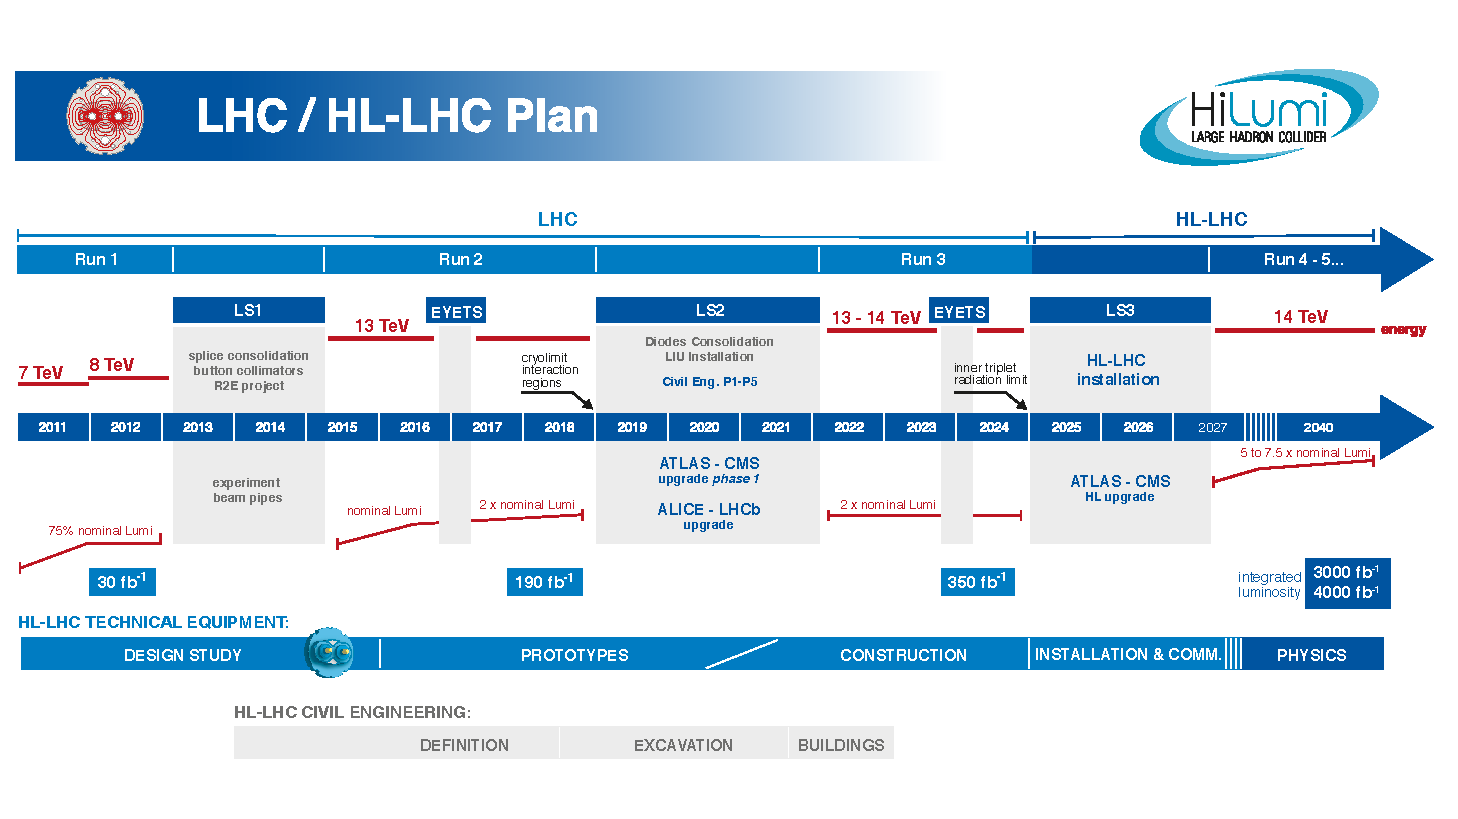
\includegraphics[width = \textwidth]{Chapter2/HL-LHC-plan-2021-1}
	  \caption{Timeline for the LHC and LHC HL projects. The periods of data taking are named Runs 
	  and, between runs, there are the Long Shutdowns (LS) in which the different facilities are upgraded.}
	  \label{fig:Chap2:HL-LHC}
\end{figure} 


Some technologies developed to upgrade the LHC to HL-LHC are: % https://www.youtube.com/watch?v=tWz12_bwqEI
\begin{itemize}
	\item Shorter bending dipole magnets are going to be installed. The current ones have a length of $15\,$m while the new are only $5.5\,$m, 
	allowing the insertion of the colliamtors
	of Figure~\ref{fig:Chap2:HL-Collimator}. The new niobium-tin dipole magnets will generate an $11\,$T magnetic field compared with the current $8.3\,$T.
	\begin{figure}
 	  \centering
 	  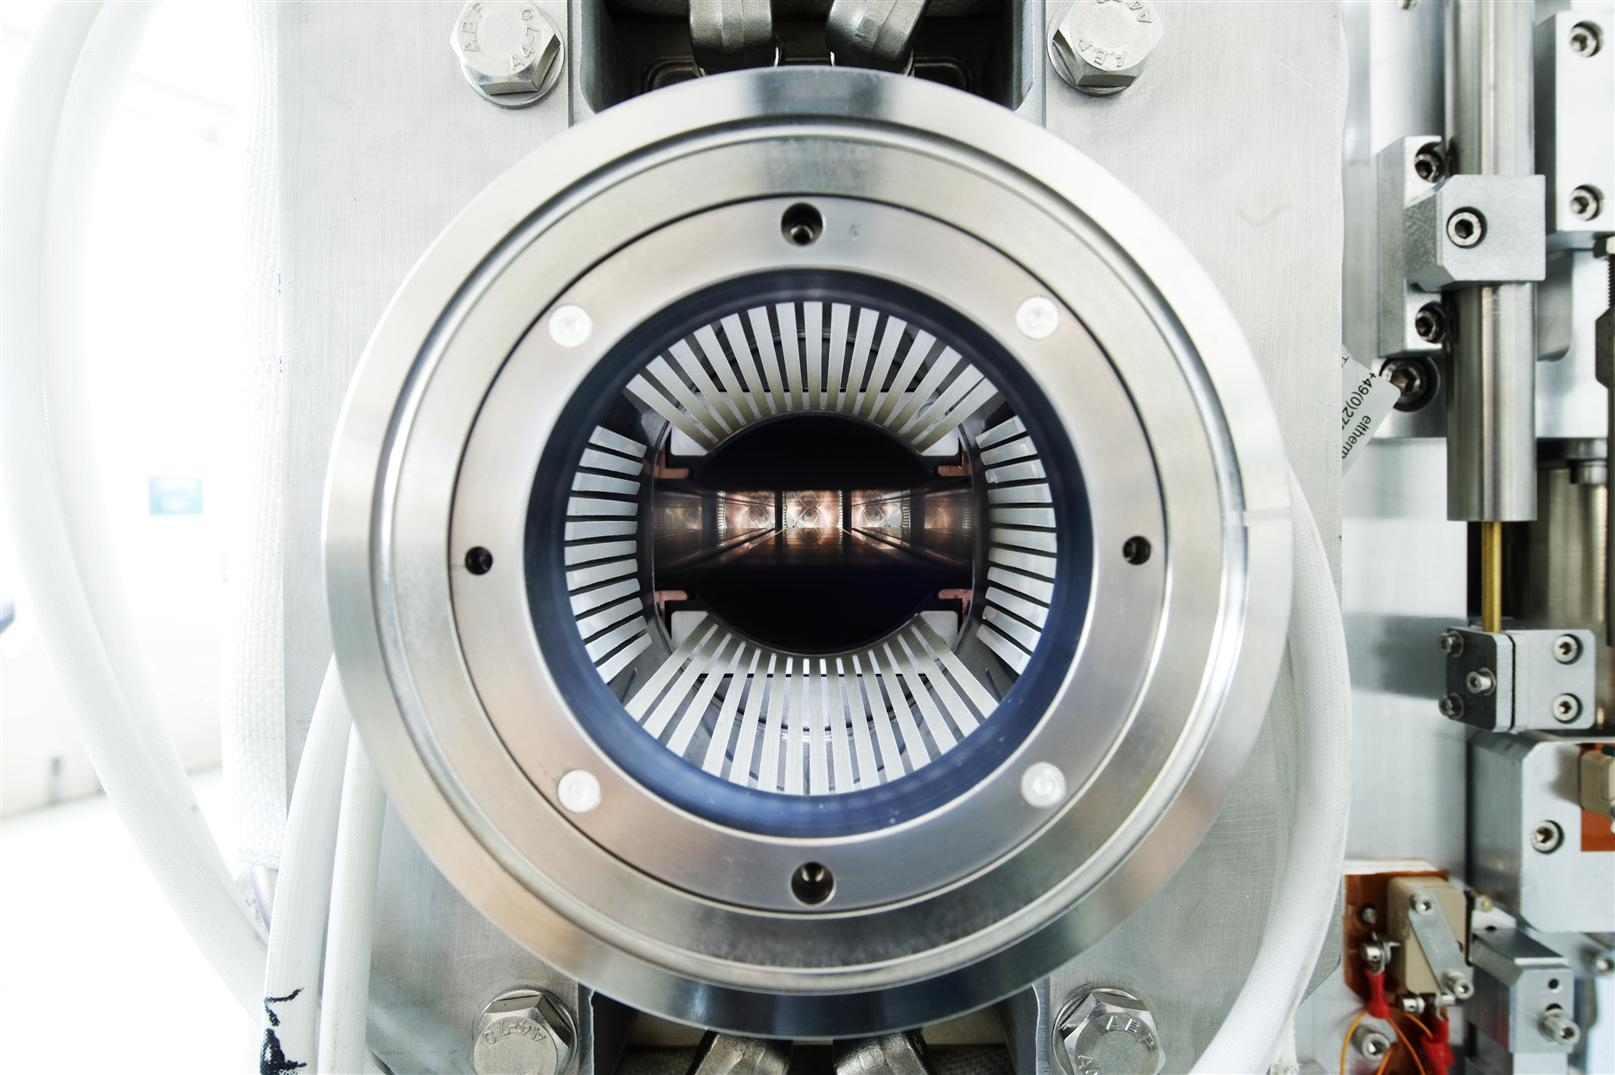
\includegraphics[width = 0.5\textwidth]{Chapter2/HL-LHC-Collimator}
	  \caption{HL-LHC Collimator.}
	  \label{fig:Chap2:HL-Collimator}
	\end{figure} 

 	\item Brand new and more powerful superconducting quadrupole magnets 
	(up to $12\,$T) made of niobium and tin will substitute the current ones ($8\,$T). These magnets will be located
	at the sides of the ATLAS and CMS detectors
	\item New Beam optics. At present, as bunches cross, the protons collide and disappear and, hence, the luminosity decreases.
	For the Run 4, in order to keep the luminosity at the same level,
	the beam focusing is designed to keep the collision rate constant.
	\item Superconducting crab cavities for giving the bunches additional transverse momentum in order to increase the probability of collisions. 
	\item New collimator sand injection magnets will also improve the performance of the machine.
	\item Thanks to the new high-temperature superconductors, currents up to $10^5\,$Amperes will be carried over long distances.
	\item New collimators that produce less electromagnetic interference with the beam are being installed. Collimators (Figure~\ref{fig:Chap2:HL-Collimator})  are
	importante because the machine protection is based on them. This elements of the accelerator absorb particles that stray from the beam trajectory and can 
	harm the devices. 
	\item The accelerator chain is improved as well with the use of the linear accelerator LINAC4 and with upgrades in the PSB, PS and PSP.	
\end{itemize}



Although increasing the collision rate of the beams is a crucial goal for CERN, improving the accelerator is not enough.
The current detectors have not been designed for HL-LHC but for the LHC and, thus, cannot handle the increased luminosity.
By increasing the luminosity while keeping the same bunch spacing, a much higher rate of collisions per bunch crossing is
achieved and this implies and higher pile-up. For Run 2, the pile up peaked around $\mu_{max}\approx70$ and that was already
quite taxing for the system in terms of tracking and reconstruction, and for Run 4 it may start around 140 and increase to 200 
interactions per bunch crossing.

Next, the main upgrades of the ATLAS detector towards de HL-LHC project are presented. 

\paragraph{Inner Tracker}
The elements in the ID receive a lot of radiation damage due the huge rate of particles hitting the detector. This radiation environment will be
even more daunting in the HL project. Therefore, the design of ATLAS (as well as all other main detectors of LHC) has to be
reviewed, especially for the most central the parts of the detector.

To deal with this, ATLAS needs much more capable trackers, therefore, the entire ID is going to be replaced
with a new ``inner tracker'' (ITk). This new detector consist on cylinder and end-caps equipped with silicon
detectors covering  a geometrical acceptance of $|\eta| < 4$.  This
expanded pseudorapidity range introduces many advantages in terms of object reconstruction
and pile-up mitigation by linking objects to the primary vertex corresponding to the hard-scatter of interest.
The new pixels sensors will be placed very close to the interaction region, where the high 
fluencies ($2\times 10^{16}\,n_{eq}$cm$^{-2}$ in the HL vs the current $10^{15}\,n_{eq}$cm$^{-2}$)
have to be tolerated while maintaining a 96\% efficiency of particle detection~\cite{CERN-LHCC-2017-021}. 

As well as the ID, the ITk is divided in two subsystems mounted in the pixel support tube: the Pixel Detectors and the strip detectors that surrounds the pixels.   
For the strips, there are four barrel layers and xix end-cap petals and for the pixels, five layers are used.


\paragraph{Calorimeters}
Due to radiation tolerance limits, the electronics for the ECAL and HCAL  have to be updated. The on-detector FE electronics 
cannot operate with the trigger rates and latencies required for the HL-LHC luminosities.
The FCAL will remain the same as in Run 2.

\paragraph{Muon Spectrometer}
The MS upgrades for the HL-LHC are focused on the muon trigger chambers. The Level-0 trigger electronics of the RPC and TCG 
will be upgraded and for the RPC the pseudorapidity coverage will be significantly increased. The front-end of the MDT is going to be 
replaced as well to address the trigger rate and latency requirements.

\paragraph{Trigger and Data Acquisition system}
\begin{wrapfigure}{R}{0.5\textwidth}
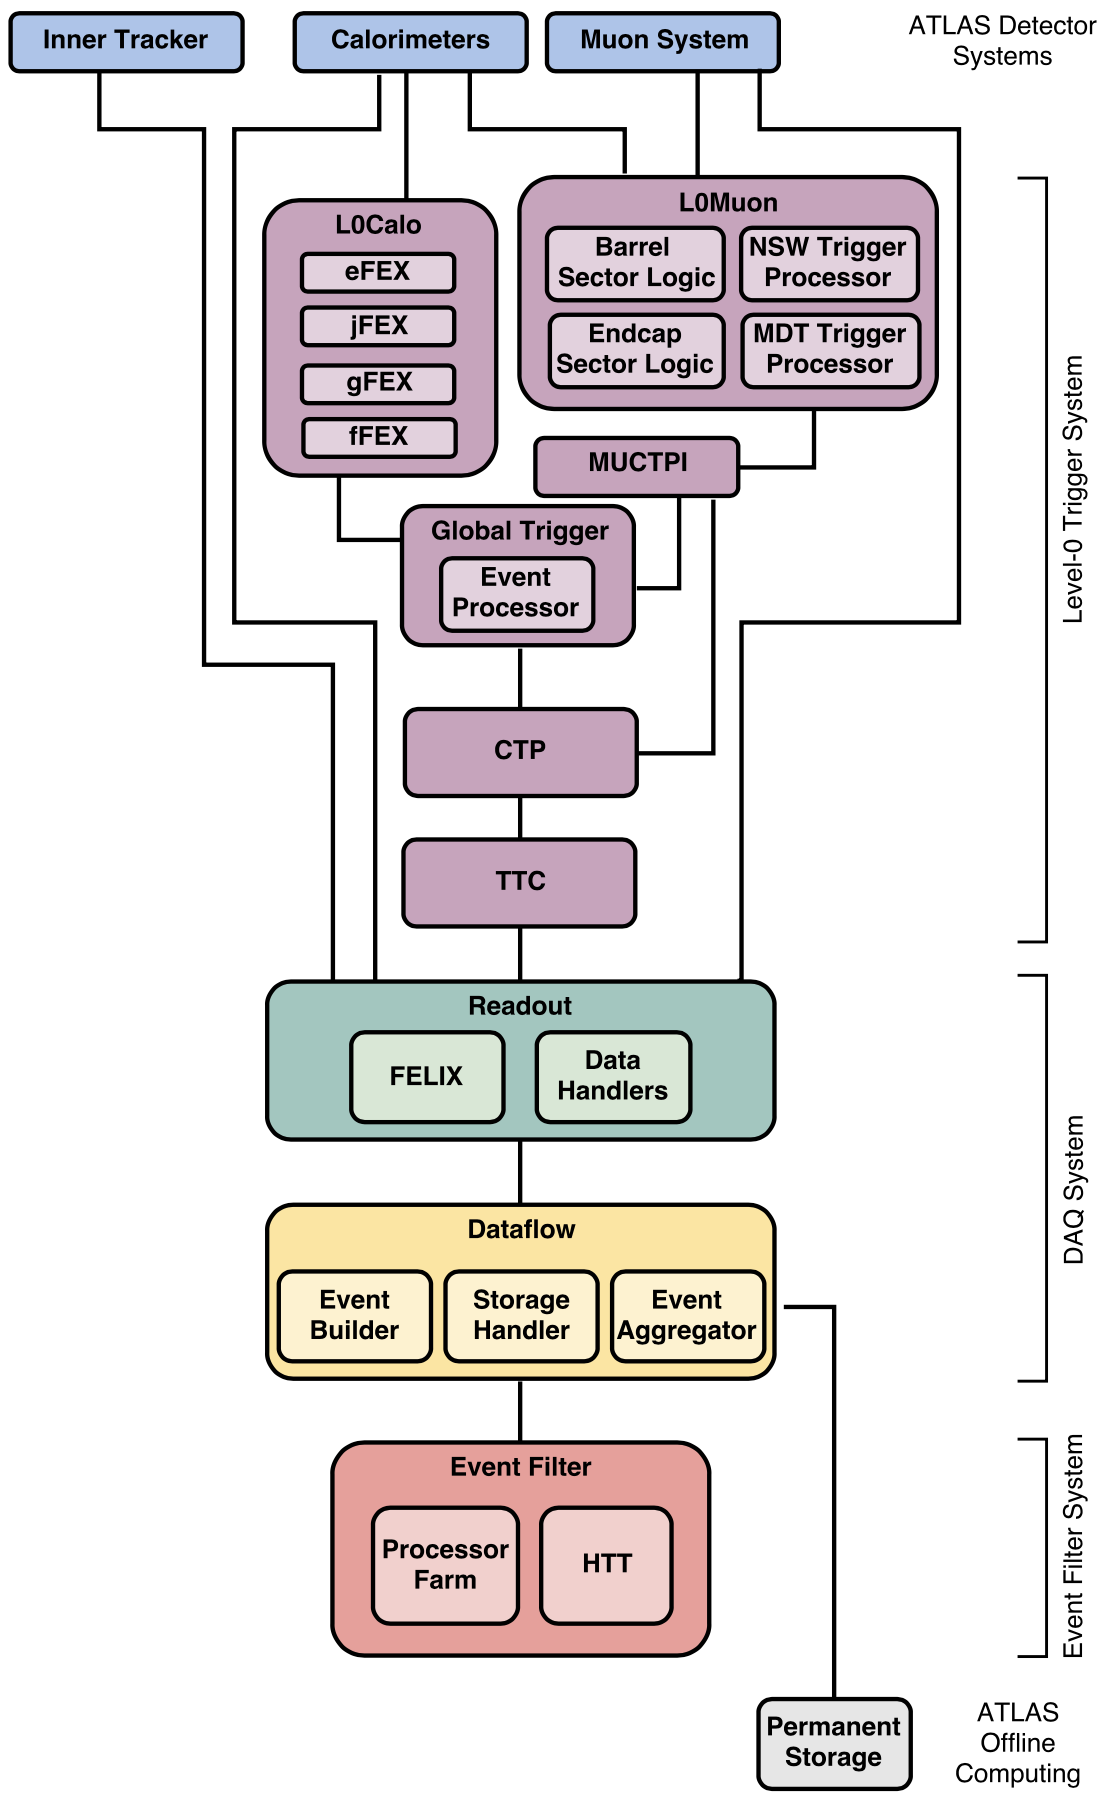
\includegraphics[width = 0.5\textwidth]{Chapter2/HL-Trigger}
\caption{	Design of the TDAQ Phase-II upgrade architecture, highlighting the organisation of the Upgrade 
		Project in three main systems~\cite{CERN-LHCC-2017-020}. Direct connections 
	  	between each Level-0 trigger component and the Readout system are suppressed for simplicity.} 
		\label{fig:Chap2:HL-Trigger}
\end{wrapfigure} 

To reconstruct the events offline, they have to be recorded in the first place, otherwise, it makes no sense to have that huge $\Pproton \Pproton$ collision rate.
 This is why while the detector hardware is being heavily upgraded, a lot of effort is being put into the trigger systems. 
The new trigger system is a multistage system that progressively takes more and more detailed information and each 
step has more time to make this decision.
It starts with $40\,$MHz input rate ($40\time 10^{6}\,$input events per second). The triggering
process starts by the Level-0 (Figure~\ref{fig:Chap2:HL-Trigger} in purple) and makes very quick decisions ($10\,\mu$s latency), reducing the rate from 40 to $1\,$MHz.
Afterwards it passes to the event filter (Figure~\ref{fig:Chap2:HL-Trigger} in orange) which takes the $1\,$MHz down to $10\,$kHz that sends to permanent storage.
The key part is that these $10\,$kHz are really the most useful  $10\,$kHz~\cite{CERN-LHCC-2017-020}. For doing so, the performance of the tracking is fundamental 
for things like particle flow identification, \MET measurements, jet tagging or tau identification.
%.........................

\end{comment}
%\pablo{From ATLAS Digest: weekly news – 11 February 2022}
%"Concerning the High Luminosity LHC, with the new schedule, LS3 will start in 2026 and the Run 4 would start in 2029. A new HL-LHC running parameters baseline is under discussion, which leads to new projections foreseeing 715/fb of pp data collected in Run 4. The beam energy for HL-LHC has also been discussed and several scenarios to reach 7 TeV per beam have been discussed. The high risk of warm-ups is a main concern and the decision will likely be postponed to the end of Run 3. Options to stay at 6.8 TeV or even backing off to 6.5 TeV to further avoid warm-ups are still on the table. Concerning the Nb3Sn inner triplets, full scale preseries prototypes are in production."  
	
	
%\subsubsection{Performance}
%\subsubsection{Challenges}

%\end{comment}  %REMOVE ENTIRE HL - LHC  : :  UNTIL HERE
\fi





%&&&%%%%%%%%%%%%%
%         	ID Alignment	       %
%%%&&&%%%%%%%%%%%      No hace falta extenderse mucho en esta sección
%\section{Alignment of the inner detector}
\section{Performance of the ATLAS detector}
\label{sec:Chap2:ID_alignement}
As vast as it is intricate, the performance of the detector  hinges crucially on the minutiae of its components and their complex interplay. 
In particular, a fundamental part for the correct operation of the ATLAS detector is the alignment of its subdetectors~\cite{ATLAS:2020ixw}. The goal of
the detector alignment is to determine the position of the detector geometry as accurately as possible in order to
correct the effects of any displacement. %In this section,
%the need of an adequate alignment is motivated, its principles discussed and my contributions presented. 
%\pablo{((los shifts no se mencionan como contribución, verdad?)}

%\subsection{Alignment of the inner detector}
As commented in Section~\ref{sec:Chap2:ID}, the ID is used to reconstruct the 
trajectories of the charged particles by combining into tracks the energy deposits
(hits) of the particles as well as identifying  primary and secondary vertices. 
These functionalities are essential for some tasks such as the lepton reconstruction
or the \bjet tagging (later described in Section~\ref{sec:Chap3:Reco:Bjets}). 
To be able to have precise and efficient tracking, the full resolution of the ID has to be exploited.
%To do so, it is crucial to know the geometry of the detector, i.e. the location and
%orientation of each of its elements. 
The detector experiences small movements that affect its geometry.
These are due to several factors such as movements during the technical stops, thermal 
expansion/contractions, % because os the cooling system, the ramping of the magnetic field, 
or any other changes in the operational conditions.
With the alignment, it is possible to account for these displacements, re-calibrate and correct their effects. %on real time"
The accuracy of the alignment algorithm is such that the position of the various detector parts may be determined
with a few microns of accuracy~\cite{ATLAS:1999vwa}.  
%This accuracy is superior to that attained by directly measuring the module placements. 
Since any misalignment of the different elements of the ID will degrade the quality of the track and object reconstruction, 
which is vital to performing any physics analysis, constant monitoring of the alignment is necessary.
During the development of this thesis, I have contributed to the alignment of the ID through the
% the refurbishment 
% of the software package for 
development of the monitoring software of the track-based ID alignment results obtained at the calibration 
loop\footnote{The calibration loop, also called 24h loop, is the process of updating the databases with the calibration results.
The calibration loop is executed every 24 hours.}.
%Cal loop = The process of database updates and primary data quality review is known as the calibration loop~\cite{ATLAS:2019fst} %and show them as a web-based service.  


%\paragraph{Importance of alignment}
%Tesis de Sebas: https://cds.cern.ch/record/2286016?ln=en
%\subsection{Alignment requirements }
\subsection{Local coordinate frame and residuals}
%\subsubsection{Local coordinate frame}
\paragraph{Local coordinate frame}\mbox{}\\
In Section~\ref{sec:Chap2:ATLAS:CoordinateSystem} the global (\textit{x, y, z}) Cartesian 
coordinate system of ATLAS is introduced. The local coordinate frame of an individual sensor
of the detector (\textit{x', y', z'}) is also given in the Cartesian system. The local system is a right-handed coordinate system
with the origin placed at the geometrical centre of the module. According to the convention,
the \textit{x'}-axis and \textit{y'}-axis are within the plane of the component and the \textit{z'}-axis
is pointing outside of this plane. The \textit{x'}-axis points to the most sensitive direction of the module. 
For the Pixel and IBL modules this is the shorter pitch side and, for the SCT, the perpendicular to the strip 
orientation. In the case of the TRT the \mbox{\textit{y'}-axis} points along the wire while the \textit{x'}-axis remains
perpendicular to both the wire and the radial direction. The local coordinates are represented schematically in 
Figure~\ref{fig:Chap2:Alignment:LocalCoordinate}.

The hits in the different subdetectors are reconstructed in the local coordinate frame of the different
modules. %While for the Pixel modules the reconstruction it is straight forward,
%in the case of the SCT the information from the two local frames associated
%to the hit are used to reconstruct it.

\begin{figure}
\centering
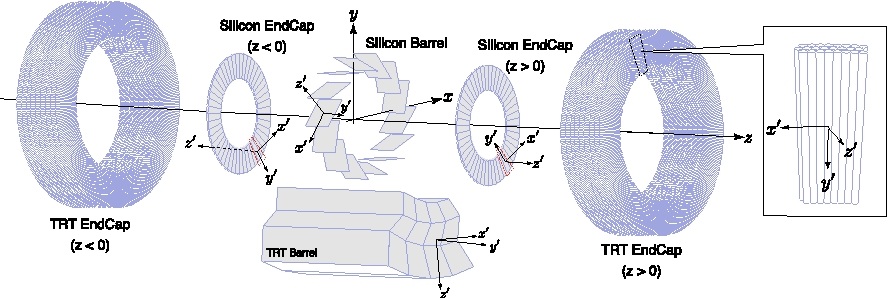
\includegraphics[width = \textwidth]{Chapter2/Alignment_LocalCoord_vect}
\caption{Schematic representation of the ATLAS global (\textit{x, y, z}) and local \mbox{(\textit{x', y', z'})} 
reference frames~\cite{ATLAS:2020ixw}. The local coordinates are shown for the Pixel, IBL, SCT and TRT. }
\label{fig:Chap2:Alignment:LocalCoordinate}
\end{figure}

%\subsubsection{Residuals}
\paragraph{Residuals}\mbox{}\\
In tracking, a residual is the distance between a hit and the intersection point of 
the extrapolated track in the sensor plane. The residual vector ($\bm{r}$) is defined as:
\begin{equation*}
	\bm{r} = (\bm{m} - \bm{e}(\bm{\tau}, \bm{\alpha}) )\, ,
\end{equation*}
where $\bm{m}$ is the vector to centre of the module and $\bm{e}(\bm{\tau}, \bm{\alpha})$
is the vector to the track intersection with the surface.  For every module crossed by the track there is a residual,
as it is shown in Figure~\ref{fig:Chap2:Alignment:Residual}. %The residuals are important since 
The alignment algorithm presented in this section is based on the minimisation of the residuals.

\begin{figure}
\centering
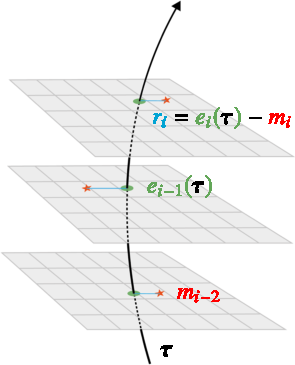
\includegraphics[width = 0.5\textwidth]{Chapter2/Alignment_residual}
\caption{Schematic representation of a charged particle crossing detector planes~\cite{ATLAS:2020ixw}.  
The red stars represent the measurements in each plane ($m_i$). The black line is the 
fitted trajectory for a given set of track parameters. The position of the intersection of the fitted 
track with the plane ($\bm{e_{i}}$) on which the $i^{th}$ measurement is made is indicated with a
green elipse. The residuals ($\bm{r_{i}}$) are represented by blue lines.}
\label{fig:Chap2:Alignment:Residual}
\end{figure}


%\subsubsection{Track parameters}
\subsection{Track parameters and degrees of freedom}
The trajectory followed by a charged particle within a magnetic field $B$ is a helix that 
can be fully parametrised by five track parameters: 
$\bm{\tau} = (d_{0},\, z_{0},\, \phi_{0},\, \theta_{0},\, q/p)$, where $d_{0}$ and $z_{0}$  
are the transverse and longitudinal impact parameters; $\phi_{0}$ and $\theta_{0}$ the 
azimuthal and polar angles of the track.  Lastly, the $q/p$ is the ratio between the particle's
charge and momentum and it measures the curvature of the tracks. 

%\subsubsection{Alignment levels and degrees of freedom}
The position and orientation of a rigid body can be described by a total of six degrees of freedom. 
This is translated into what is known as alignment parameters 
$\bm{\alpha} = (T_{x},\, T_{y},\, T_{z},\, R_{x},\, R_{y},\,R_{z})$. These correspond to the
three translations with respect to the origin of the local reference frame ($T_{x,y,z}$) 
and three rotations ($R_{x,y,z}$) around the local Cartesian axes. 



\subsection{Track based alignment}
%The distance between the hits and the fitted track should be null if the detector was perfectly aligned, 
%and the residual distribution would be centred at zero and have a width that corresponded to the 
In the case of a perfectly aligned detector, the distribution of residual vectors would be centred at 
zero and have a width that corresponds to the
module resolution. Therefore, any deviation in the residual distribution indicates a 
misalignment of the detector. 


\begin{figure}[h]
\centering
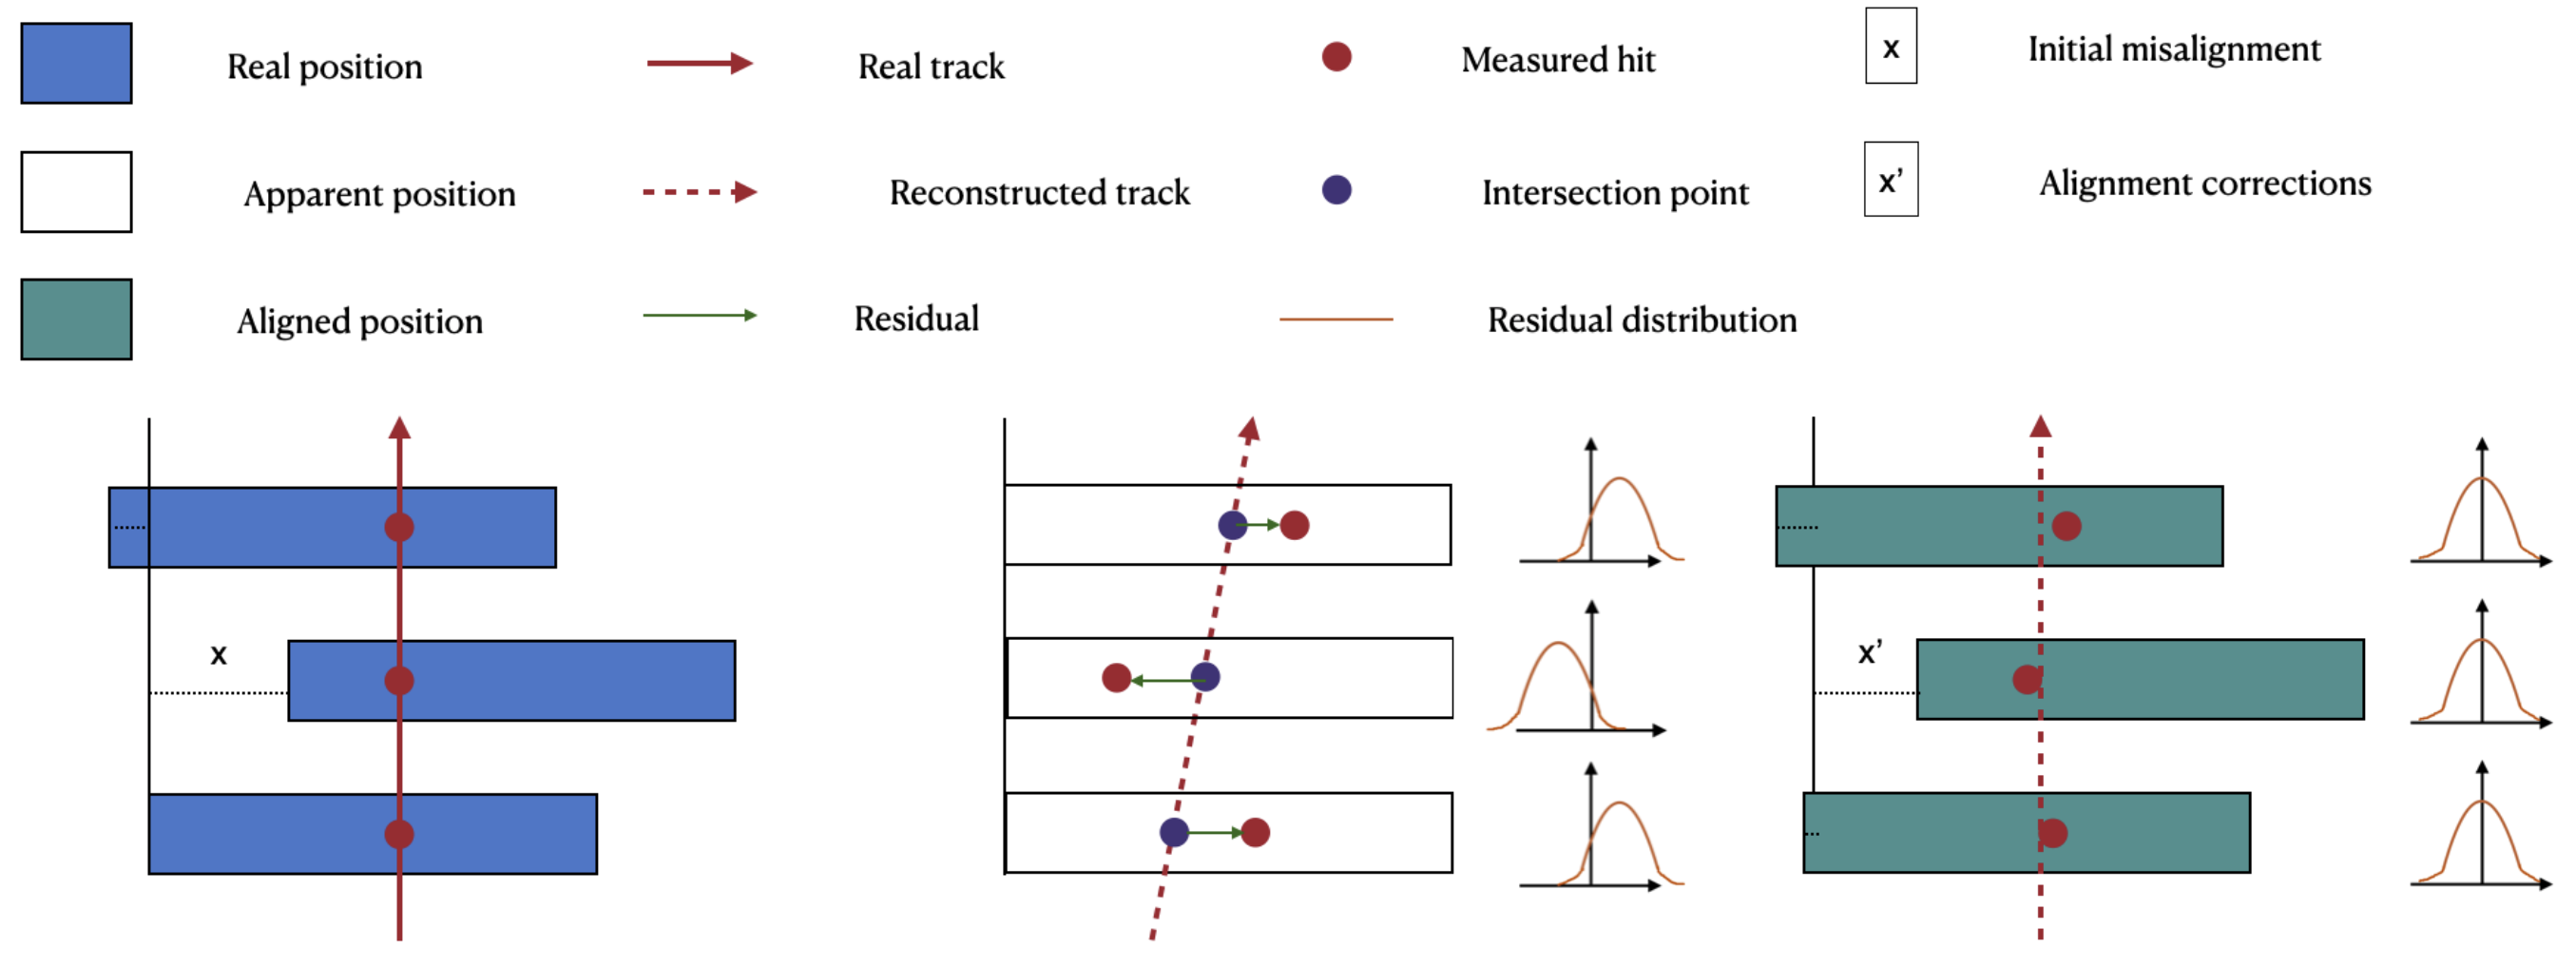
\includegraphics[width = \textwidth]{Chapter2/AlignmentChain_ToBeVectorised}
\caption{Alignment procedure scheme where each rectangle represents a detector module. 
	%The left panel represents the real (unknown) position of the detector modules and the particle track.
	%The middle panel shows the initially-expected position of the modules and the reconstructed track.
	%The right panel exemplifies how the position of the detectors is updated to resemble the real one
	%after determining the actual position of the modules provided by the track-based alignment procedures.
	%This update is done by the track-based alignment procedure.   \pablo{ I need to vectorise this image} 
	}
\label{fig:Chap2:Alignment:Chain}
\end{figure}

A schematic description of the alignment chain is illustrated in Figure~\ref{fig:Chap2:Alignment:Chain}.
The blue rectangles on the left panel of this figure represent the true position of 
the detector modules. A charged particle produces hits in each module, 
which are marked with red dots. The track of the particle is marked with a red line. The $x$ distance
is the deviation of the module from its apparent position (considering there is no misalignment). In the middle panel, the white rectangles
represent the apparent position of each module. It can be seen that the real and the 
apparent positions are not the same, differing by an unknown distance $x$. This deviation leads to a discrepancy between 
the reconstructed tracks and the true ones. The residuals in the middle panel are represented by a green
line, which corresponds to the difference between the recorded track (red dots) and the reconstructed
one (blue dots). The residual distributions in this panel are displaced from zero, indicating a misalignment.
The purpose of the alignment algorithm is to centre these distributions in zero by minimising these residuals.
As a result of the alignment procedure, the position of the detectors has been updated a distance $x'$ 
for each module. After this, the new expected position of the modules (green rectangles) is much closer to 
the real one and, hence, the residuals are more centred at zero. Anyhow, this is not perfect and the different
$x'$  are not all equal to $x$. To improve the precision, the alignment procedure is repeated iteratively 
with the calibration loop until the convergence of the corrections.

\subsubsection{Global $\chi^2$ algorithm} %1 or 2 pages explaining the algorithm
To correct the position of the ID, the alignment constants ($\bm{\alpha}$) are obtained as result 
of the minimisation of a $\chi^2$ function. This function is built from the track-hit residuals:
\begin{equation*}
	\chi^{2} =  \sum_{e}\sum_{t} \sum_{h} \left( \frac{r_{t,h}(\bm{\tau}, \bm{\alpha})}{\sigma_{h}} \right)^{2},
\end{equation*}
where the index $e$ runs over the selected events, the index $t$ runs over the reconstructed 
tracks with one event, and the index $h$ is the set of hits associated to each 
track $t$ in each event. The residual of each hit associated to track $t$ is $r_{t,h}$ and $\sigma_{h}$ is the uncertainty of the measured hit.
In vector notation, the $\chi^2$ function can be expressed as:
\begin{equation*}
	\chi^{2} =  \sum_{e} \sum_{t} \bm{r}^{T}\Omega^{-1} \bm{r},
\end{equation*}
where $\Omega$ is the covariance matrix of the corresponding measurements
and $\bm{r}$ the residual vector. 
The alignment constants $\bm{\alpha}$ are those that minimise the $\chi^2$ and, therefore,
first and second derivatives of $\chi^2$ with respect $\bm{\alpha}$  are used. %The sum
%on $t$ runs over all tracks. 
%Defining the derivative $G = d \bm{\tau}/\bm{r}%
\begin{equation*}
	\frac{d \chi^{2}}{d \bm{\alpha}} =
	 \sum_{e} \sum_{t} \left[  \left(\frac{d  \bm{r} }{d \bm{\alpha}} \right)^{T} \Omega^{-1} \bm{r} \right]^{T} +
	 \sum_{e} \sum_{t} \left[  (\bm{r}^{T} \Omega^{-1} \left( \frac{d \bm{r}}{d \bm{\alpha}} \right) \right]
	= 0
\end{equation*}
It is worth to remark that $\bm{r}$ and $\Omega$ are defined for all events and tracks with each event, so the sum will 
accumulate the residuals from all considered tracks from all the events in the data sample. The last 
expression can be simplified taking into account that $\Omega^{-1}$ is symmetric (i.e. $(\Omega^{-1})^{T} = \Omega^{-1}$) and it takes the form:
\begin{equation}\label{eq:Chap2:Chi2_A}
	\frac{d \chi^{2}}{d \bm{\alpha}} = 2 \sum_{t} \left(\frac{d  \bm{r} }{d \bm{\alpha}} \right)^{T} \Omega^{-1} \bm{r} = 0 \, .
\end{equation}
Now, since $\bm{r} = \bm{r}(\bm{\tau}, \bm{\alpha})$, partial derivatives have to be taken into account:
\begin{equation*}
	\frac{d  \bm{r} }{d \bm{\alpha}} =
	 \frac{\partial  \bm{r} }{\partial \bm{\tau}} \frac{d  \bm{\tau} }{d \bm{\alpha}} + 
	  \frac{\partial  \bm{r} }{\partial \bm{\alpha}} 
\end{equation*}
Inserting this into equation~\ref{eq:Chap2:Chi2_A}, the condition for minimising the $\chi^{2}$ turns 
to be:
\begin{equation}\label{eq:Chap2:Chi2_B}
	\sum_{t} \left(\frac{\partial  \bm{r} }{\partial \bm{\tau}} \frac{d  \bm{\tau} }{d \bm{\alpha}} + 
	  \frac{\partial  \bm{r} }{\partial \bm{\alpha}} \right)^{T} \Omega^{-1} \bm{r} = 0 \; .
\end{equation}

%\begin{comment}
%Here, the term $d\bm{\tau} / d\bm{\alpha}$ is of particular importance since its contains
%the relationship between the track and alignment parameters, and it will determine 
%the difference between the \textit{Local}  and \textit{Global} $\chi^{2}$ algorithms.
%
%If the algorithm assumes that track parameters do not depend on the alignment, i.e.
%$d\bm{\tau} / d\bm{\alpha} = 0$, it is the so-called \textit{Local} $\chi^{2}$ algorithm.
%In this case, the total derivative in equation~\ref{eq:Chap2:Chi2_A} is reduced to 
%the partial derivative of  \with respect to the 
%On the other hand, the \textit{Global} $\chi^{2}$ is based on the assumption that 
%the track and alignment parameters are dependent. 
%\end{comment}

The alignment parameters that satisfy the relation in equation~\ref{eq:Chap2:Chi2_B} are found 
by an iterative process consisting on evaluating the first and second derivatives
of the $\chi^{2}$ with respect to the current iteration alignment parameters, $\bm{\alpha}_{0}$.
Since the derivative terms of equation~\ref{eq:Chap2:Chi2_B} depend on $\bm{\alpha}$ itself, 
the procedure is repeated until a convergence criteria is achieved.
To get the set of alignment parameters corrections ($\delta \bm{\alpha}$), the alignment parameters
can be written as $\bm{\alpha} = \bm{\alpha}_{0} + \delta\bm{\alpha}$. 
%Assuming that the correction is close to the actual alignment parameters, a Taylor expansion
% is performed. 
%The minimisation condition in equation~\ref{eq:Chap2:Chi2_B} requires to calculate
%the term $\partial  \bm{r} / \partial  \bm{\tau}$. 
Therefore, from the equation~\ref{eq:Chap2:Chi2_A}, the following relation is obtained 
 \begin{equation}\label{eq:Chap2:Chi2_C}
 	\left[ \sum_{e}\sum_{t} \left( \frac{d\bm{r}}{d\bm{\alpha}_{0}}\right)^{T}\Omega^{-1}\left( \frac{d\bm{r}}{d\bm{\alpha}_{0}}\right)\right]\delta\bm{\alpha}
	+
	\sum_{e}\sum_{t} \left(\frac{d\bm{r}}{d\bm{\alpha}_{0}}\right)^{T}\Omega^{-1}\bm{r}(\bm{\tau}_{0}, \bm{\alpha}_{0}) 
	= 0 \,.
\end{equation}
Hence, from this equation it is possible to define the alignment matrix ($M_{a}$) and vector ($v_a$) as:
\begin{equation*}
	M_{a} = \sum_{e}\sum_{t} \left(\frac{d\bm{r}}{d\bm{\alpha}_{0}}\right)^{T}\Omega^{-1}\frac{d\bm{r}}{d\bm{\alpha}_{0}} \, ,
\end{equation*}
\begin{equation*}
	v_{a} = \sum_{e}\sum_{t} \left(\frac{d\bm{r}}{d\bm{\alpha}_{0}}\right)^{T}\Omega^{-1}\bm{r}(\bm{\tau}_{0}, \bm{\alpha}_{0})  \, .
\end{equation*}
And the relation in equation~\ref{eq:Chap2:Chi2_C} can be rewritten as $M_{a} \delta\bm{\alpha} + v_{a} = 0$, implying
that $\delta\bm{\alpha} = -M_{a}^{-1}v_{a}$. The alignment parameters $\bm{\alpha}$ 
are iteratively derived until convergence is reached. The iterative expression is $\bm{\alpha}_{N} = \bm{\alpha}_{N-1}+\delta\bm{\alpha}_{N}$,
where $N$ is the current iteration.

The Global $\chi^2$ algorithm encompasses all alignable modules, factoring in their intercorrelations, 
which makes solving equation~\ref{eq:Chap2:Chi2_C} computationally challenging. Given the intricate granularity 
and sophistication of the ID, alignment can be undertaken at various hierarchical levels. These levels correspond 
to the ID's assembly structure, with the complexity ascending progressively. This gradation is realised 
by mapping the residuals, initially computed at the module level, onto more expansive surfaces 
corresponding to broader ID structures. The subcomponents of the ID are categorised into five tiers (see Table~\ref{table:Chap2:AligntLvls}), 
ranging from a count of 7 structures to $351\times 10^{3}$, based on their structural composition. 

\begin{table}[h]
    \centering
    \resizebox{\textwidth}{!}{%
    \begin{tabular}{c c c}
        \toprule
        Level 	& Description 									& Number of structures \\ \midrule
        1     		& IBL, Pixel, SCT end-caps, TRT barrel and end-caps	& 7		\\
\multirow{2}{*}{Si2} & IBL Layers, Pixel end-cap disks and barrel layers, & \multirow{2}{*}{32} \\
      & \multicolumn{1}{l}{SCT end-cap disks and barrel layers} &                      \\
        Si3   		& IBL modules, Pixel modules and SCT modules		& 6112	\\
        TRT2  	& TRT barrel modules and end-cap wheels			& 176	\\
        TRT3  	& TRT straw tubes								& $351\times 10^{3}$	\\
        \bottomrule
    \end{tabular}}
    \caption{Alignment configuration split by levels used during Run 2 data-taking period.}
    \label{table:Chap2:AligntLvls}
\end{table}
 




 
 %Additionally, the track fit can be further improved by adding supplementary constraining terms that account 
% for the effects of multiple Coulomb scatterings of the particle with the detector.

%\subsubsection{Weak modes}
% Igual me da perecita explicar lo weak models :D



%\subsection{Alignment towards Run 3}
%\pablo{Preguntar a Paolo sobre esto. ¿realmente quiero escribir sobre este tema?}
%\subsubsection{Pseudo-real-time-online monitoring}

%\subsection{Web-based display for alignment monitoring}
\subsection{ID alignment monitoring}
% Twiki: https://twiki.cern.ch/twiki/bin/viewauth/AtlasComputing/AlignmentWebDisplayHowTo
% Git repository: https://gitlab.cern.ch/atlas-idalignment/InDetAlignmentWebMonitor
The ID Alignment Monitoring Web Display (Figure~\ref{fig:Chap2:Alignment:WebDisplay}) is an application intended for monitoring the track-based
alignment results obtained at the calibration loop for the ID. It helps to evaluate the computed 
alignment corrections as well as many graphical distributions directly related to the performance. 
%\pablo{I have not explained what the calibration loop is :(}

The web application is structured with a server overseen by the ATLAS Distributed Computing.
It incorporates a suite of backend scripts designed for generating distributions, 
refreshing the data, and managing HTTP requests from the users. The frontend allows to the user
to interact with the application by requesting alignment-related information.  
This tool is integrated within Athena\footnote{Athena represents a specific implementation of a component-based architecture, drawing inspiration from LHCb's Gaudi~\cite{Mato:1998gfa}. It is tailored for an extensive variety of physics data-processing tasks.}, the established software framework for ATLAS~\cite{Duckeck:2005rb}.


%The web application consists of a server, managed by ATLAS Distributed Computing, and a
%collection of scripts to produce distributions, update the information and handle the http requests.
%It is available at Athena\footnote{Athena is a
%concrete realisation of a component-based architecture (based on LHCb's Gaudi~\cite{Mato:1998gfa}) 
%which was designed for a wide range of physics data-processing applications.}, 
%the software framework for ATLAS~\cite{Duckeck:2005rb}. 

%Part of my personal work has consisted in writing the code for both
%the frontend and backend of the ID Alignment Monitoring Web Display. 
A segment of my responsibilities encompassed the development and implementation
of both the client-side (frontend) and server-side (backend) 
code for the ID Alignment Monitoring Web Display. 
%The implemented design ...
%From an outdated set of scripts, the backend of the application has been remodelled. In the new version
%all the code duplicities have been suppressed by defining classes, methods and functions. 
%The same lines where written over and over again.

%\begin{comment}
%Several new functionalities have been added, to name some:
%	\item The web uses the standard Athena setup instead of loading a 
%	bash script in which the Athena version had to be hardcoded.
%	\item Debug levels using ATLAS printing style methods have been implemented.
%	\item Now it is possible to update a single run or list of runs while in the 
%	previous version it was necessary to execute the program over all runs again.
%	\item It is not necessary to hardcode the year anymore, it is automatically now.
%	\item Depending on which run was decided to plot, it was necessary to hardcode
%	the year in he scripts. Now the web tool allows to do this from its interface.
%	\item In the new version it is possible to access the ATLAS Metadata Interface\footnote{
%	Known as AMI, it is a generic software ecosystem for retrieving scientific data by metadata 
%	criteria. It allows to search for real and simulated data by metadata criteria as well as browse, view, 
%	compare and create ATLAS AMI-Tags.} information.
%	\item The runtime of the code has been speed up by performing the execution in a single loop in contrast
%	to the two-loops structure of the previous version. 
	% Before we used to make a loop over all runs (\texttt{runListInTestingFolder}) 
	% and if for a certain run the info had to be updated or it was new, we added this 
	% run to a list (\texttt{RunsWithNewData}) over which we made a second loop fill 
	% the information. Now we do everything in a single loop over all runs filling the 
	% info on the fly if necessary. This makes the code more clean, clear and 
	% understandable.
%
%\end{comment}

In the enhanced version of the Alignment Monitoring Web Display, several advancements 
and refinements have been made compared to its predecessor:
\begin{itemize}
	\item Integration with the standard Athena setup has been achieved.
	\item Conformity to ATLAS styling and debugging standards has been 
	ensured~\cite{AtlasDesign2023}. %Eisenhandler:1110290
	These standards are a compendium of rules, recommendations and advice for 
	presenting the information within the ATLAS collaboration. The web presents
	a professional visual identity that is both memorable and easy to recognise.
	\item Enhanced efficiency in execution has been introduced by allowing updates 
	for individual runs or batches of runs.
	\item The system now dynamically updates the year, eliminating the necessity for 
	manual hardcoding.
	\item Through frontend interactions, users can now select any run for visualisation,
	thereby eliminating hardcoded dependencies.
	\item Users can now query the ATLAS Metadata Interface\footnote{Known 
	as AMI, it is a generic software ecosystem for retrieving scientific data by metadata 
	criteria. It allows to search for real and simulated data by metadata criteria as well as browse, view, 
	compare and create ATLAS AMI-Tags}  for relevant data.
	\item Algorithmic optimisation has been performed, streamlining code execution through a singular iterative loop.
	\item The codebase has been refined to eliminate redundancies and duplicities with respect
	to the previous versions.
\end{itemize}


\begin{figure}[h]
	\centering
  	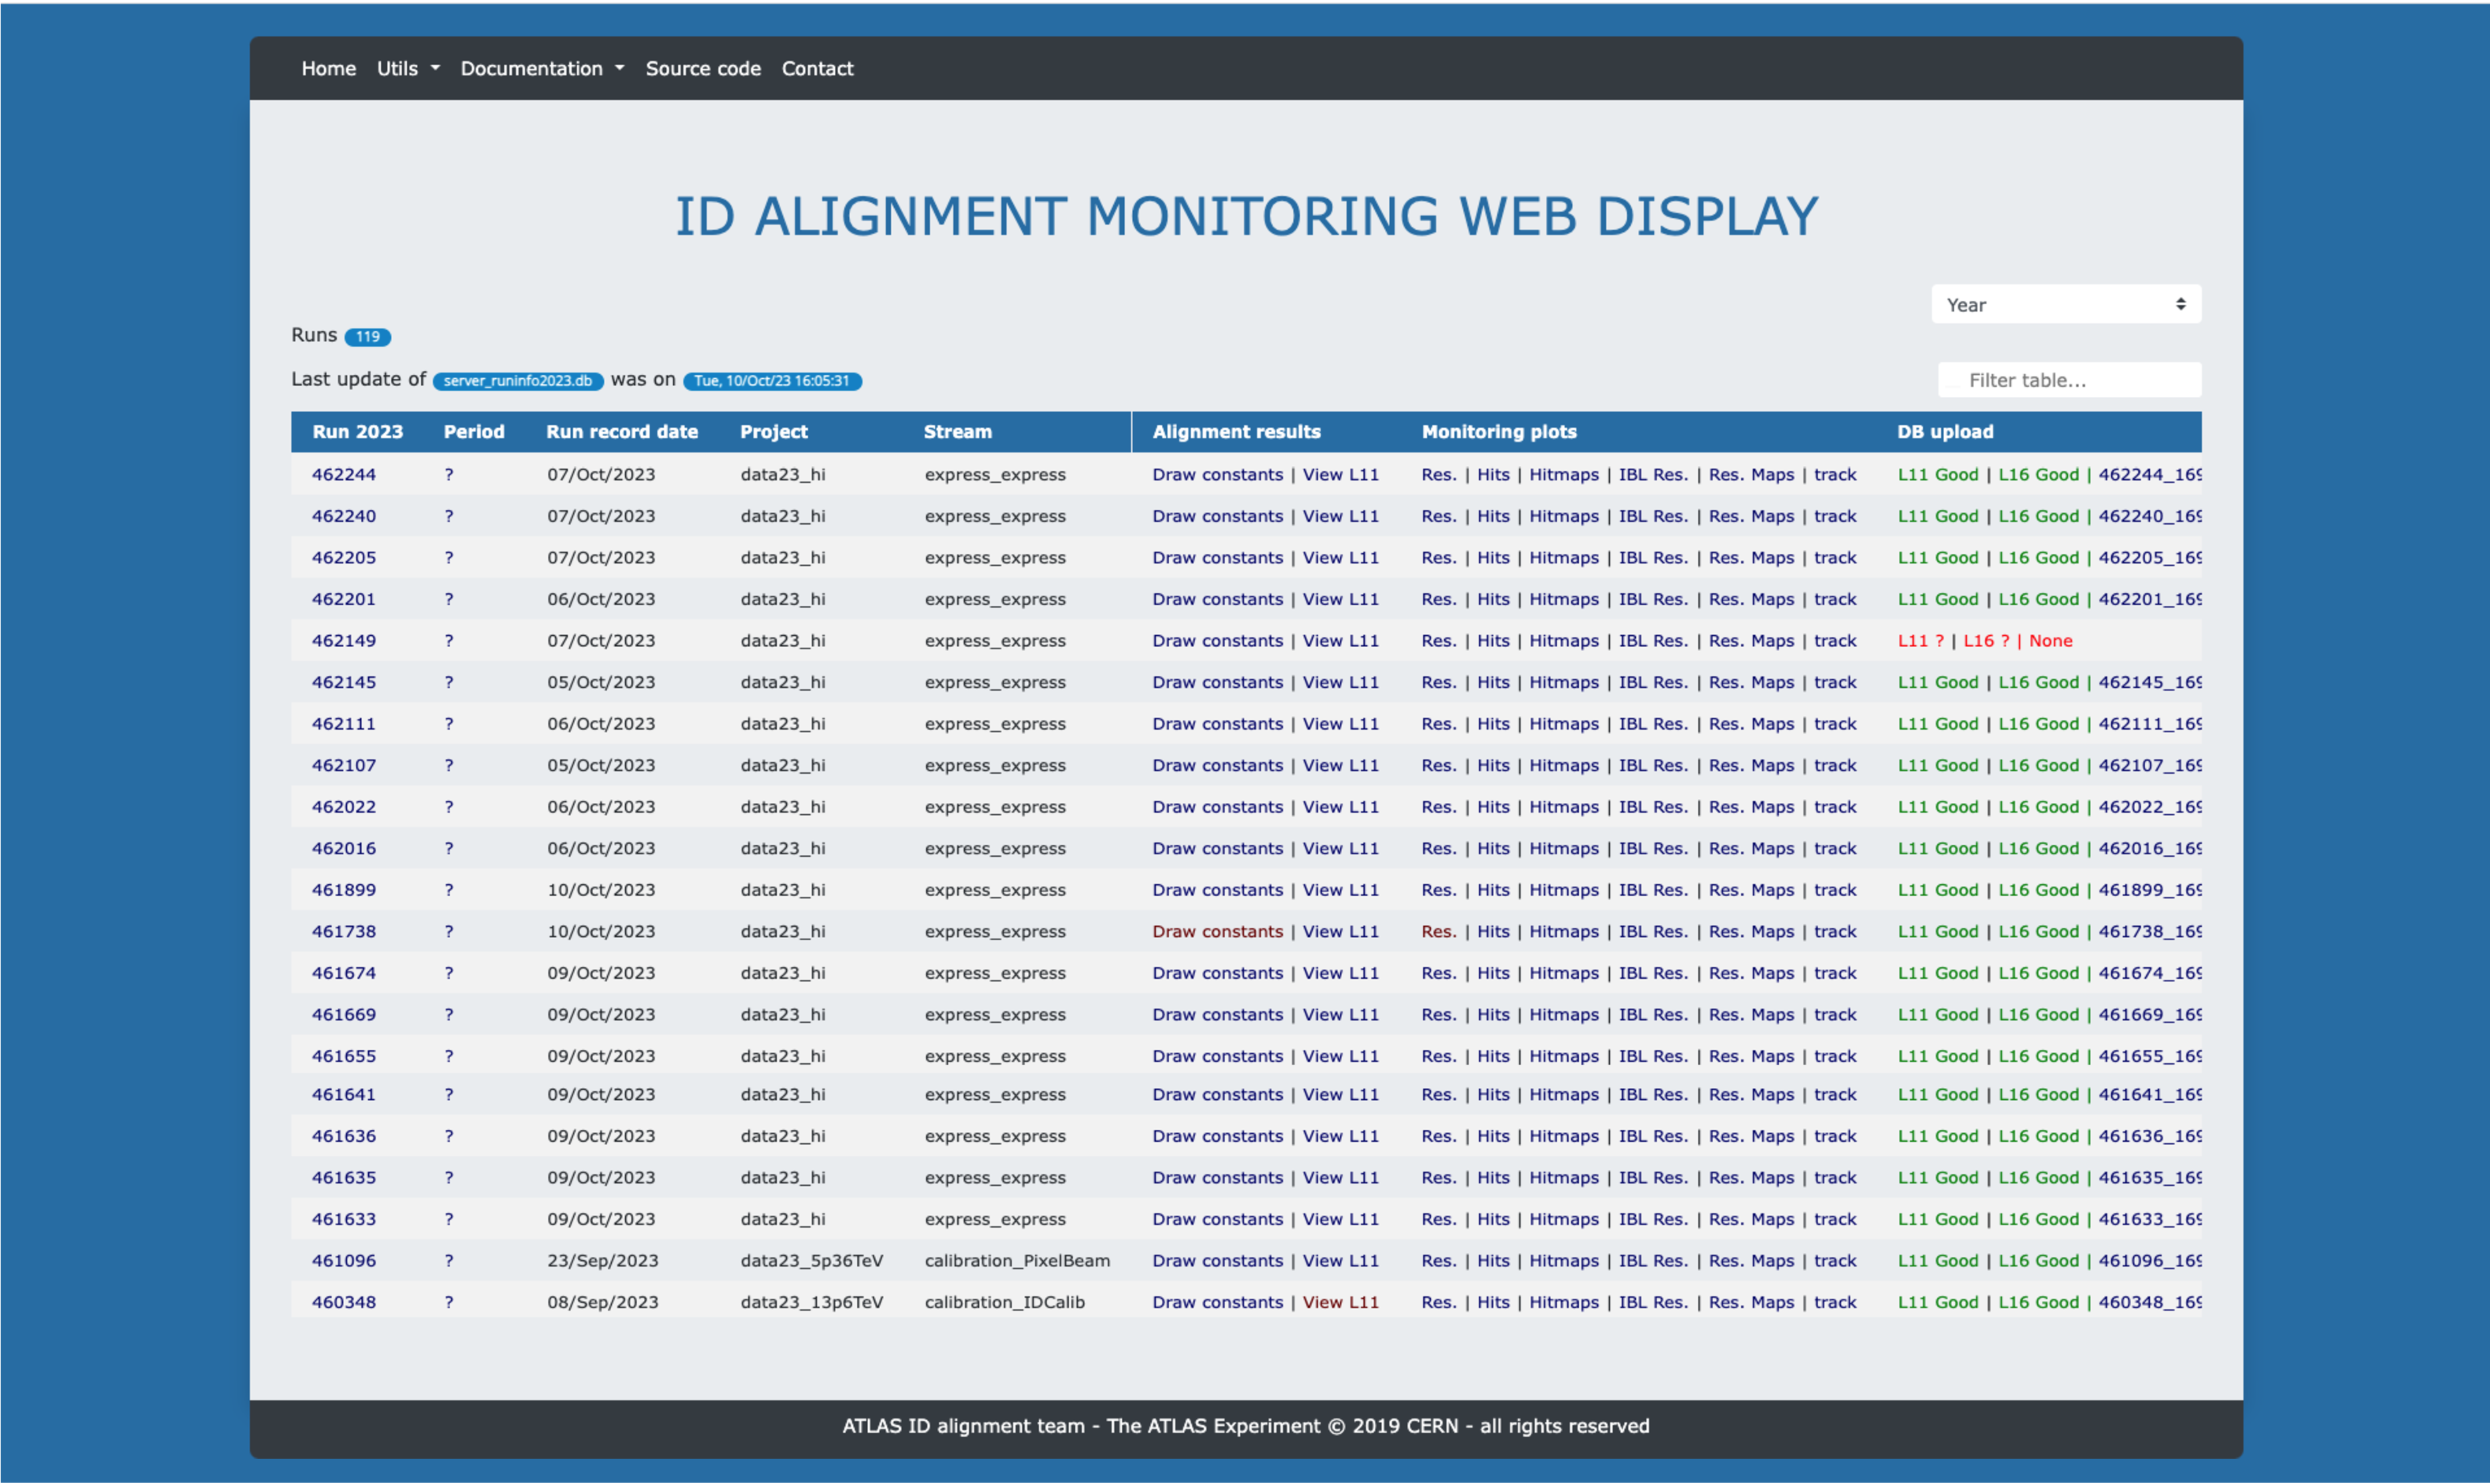
\includegraphics[width=0.9\columnwidth]{Chapter2/WebDisplay_Bueno}
	\caption{Main page of the ID Alignment Monitoring Web Display on wide resolution screen. The
	monitor presents the runs and allows to access the alignment information and plots. Queries can be used
	to filter the runs presented.}
	\label{fig:Chap2:Alignment:WebDisplay} 	
	% https://atlasalignment-dev.cern.ch/webapp/
\end{figure}

The graphical interface and layout of the application are designed to adhere to the ATLAS 
style guidelines. The frontend code foundation leans on the CherryPy library~\cite{CherryPyDoc}, 
an object-oriented web framework developed in Python.
This choice is motivated by its simplicity and good capabilities. 
However, it is pertinent to note that contemporary web 
development trends see an inclination towards more 
feature-intensive Python web frameworks, such as Django and Flask.
 As a result, CherryPy, while still effective, might not be the premier choice for newer undertakings.

Supplementing the core functionalities, the application seamlessly integrates 
CSS, HTML~\cite{Berners-Lee:2639699}, and Java.  %~\cite{MDNCSS2023}~\cite{javaTechInsider1995}
The revamped web interface provides users with an intuitive mechanism to determine the displayed information. 
A pivotal enhancement is its responsive design\footnote{Responsive design in web programming refers to the 
approach of creating web pages that automatically adjust and optimise their layout and content based on the 
screen size and orientation of the device on which they are viewed.}, 
enabling impeccable adaptability across devices, from desktops to mobiles. 
This feature ensures that shifters\footnote{The term ``shifters''  refers to the individuals who are assigned to monitor 
the ATLAS detector and its data-acquisition systems during data-taking periods. In this context, I am referring to to 
the ID alignment shifters.} can effortlessly access alignment data from any device, optimising their workflow. 
This mobile-centric adaptability is powered by Bootstrap~\cite{EfroTibs93}, a leading CSS framework renowned for 
championing responsive, mobile-first frontend web development.

Other enhancements in the frontend include:
\begin{itemize}
	\item The navigation bar has been enriched, offering a wider array of options 
	for seamless navigation.
	\item A sophisticated filter mechanism has been incorporated, enabling users 
	to exclusively display runs that meet specific criteria.
	\item An intuitive selector is now integrated, showcasing the years available 
	in the database for hassle-free selection.
	\item Accessibility has taken a front seat, with the introduction of features like
	the hover selector, a grid-based display for plots, and a modal image gallery (lightbox) that simplifies plot navigation. All these features have been meticulously crafted using CSS\footnote{CSS was first proposed on 1994 at CERN.}. %~\cite{howcomeCascade1994}
\end{itemize}

Cumulatively, these advancements not only bolster the execution speed of the application but also
provide access to more information, and allow to easily manage and access the desired data.  
The ID Alignment Monitoring Web Display that I engineered is currently being used actively by members of 
the ATLAS collaboration to monitor the ID alignment during Run 3 as well as the reprocessing of the data 
of Run 2. 
It has significantly simplified the monitoring of alignment, making the task 
more efficient and user-friendly. 

%\pablo{Escribe párrafo conclusiones !! :: decir que se está utilizando actualmente y que gracias a ello me cualifiqué como autor de ATLAS.}

%Regarding the frontend, it has been developed from the scratch. 
%The aesthetics of the web page is the most visible change in the monitor display.
%The frontend code is based on CherryPy~\cite{CherryPyDoc}, an object-oriented web application framework using 
%the Python programming language, and also includes CSS, HTML and Java.
%The enhanced web display allows to easily choose which information is shown.  
%The web has been designed to adapt to mobile devices, 
%as Figure~\ref{fig:Chap2:Alignment:WebDisplay_mobile} shows. To do so, it uses Bootstrap,
%a CSS framework directed at responsive, mobile-first frontend web development .


%The navigation bar of the web has also being improved, having a better organisation, more 
%option and, if the browser screen is narrowed, it collapses into a desplegable sidebar.
%A filter has been added that allows to show only the runs that follow the desired specific criteria.
%A desplegable to select the years has been included, the script reads from the available 
%years in the database. A year selector presentes the possible years via a script that
%reads the available data. The hoover function highlights the text as the pointer goes
%over it. The plots are presented in a cleaner way using grid view to select the plot of interest
%and light boxes to highlight them. The legends of the plots have also been modified
%to remove duplicated items.




%\begin{figure}[htp]
%  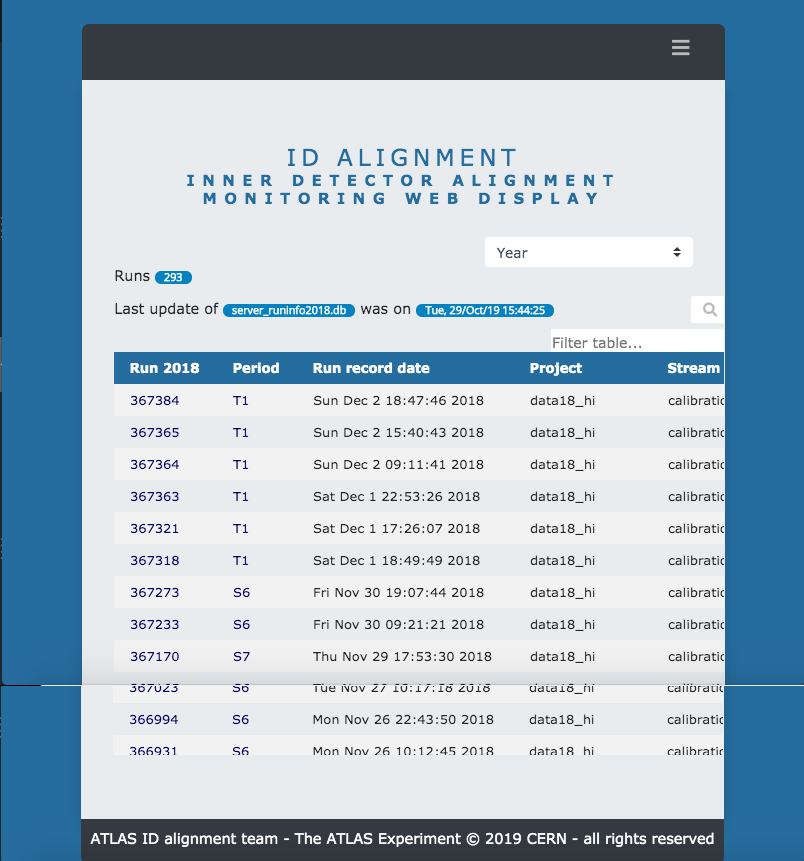
\includegraphics[width=0.5\columnwidth]{Chapter2/WebDisplay_Final_Mobile.jpg} \hspace{0.3 cm}
%  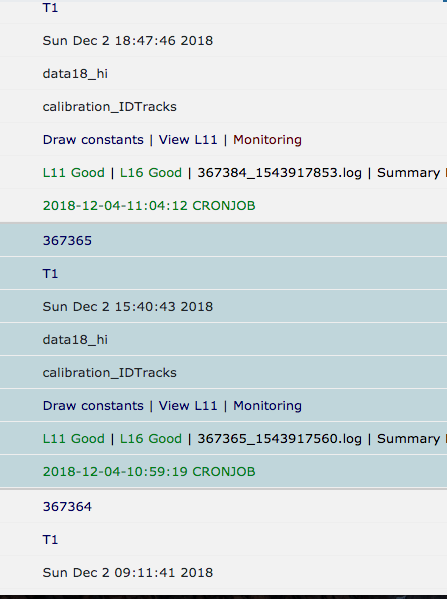
\includegraphics[width=0.4\columnwidth]{Chapter2/WebDisplay_Final_Mobile_3.png}
%\caption{Main page of the ID Alignment Monitoring Web Display on narrow screens 
%such as the ones of a mobile device.}
%\label{fig:Chap2:Alignment:WebDisplay_mobile}
%\end{figure}



%\subsection{Alignment results during Run 2}
%\pablo{Here I should find some plot that summarises the results of the alignment and I must 
%highlight the importance of alignment to perform the analysis.}




%&&&%%%%%%%%%%%%%%%%%%%%%%%%%%%%
%      	LHC - Energy and Cross-section        %
%%%&&&%%%%%%%%%%%%%	%%%%%%%%%%%%%
%\section{Basic concepts for accelerator physics}
%\label{sec:Chap2:LHC:lumi}
%\pablo{Aún hay que ver por dónde pongo esta sección,}

%In this section are covered some fundamental concepts in accelerator physics. 
%These concepts include energy, luminosity, and cross section. Understanding 
%these elements is crucial for comprehending the dynamics of particle accelerators 
%and the results obtained from particle-physics experiments. 


\begin{comment}
%%%%%%%%%%%
%        Energy         %
%%%%%%%%%%%
\subsection{Energy}
\label{sec:Chap1:LHC:Energy}
%\paragraph{Energy}\mbox{}\\
Another name to refer to the field of Particle Physics is ``high energy physics''. Particles such as the Higgs boson or the top quark are 
more than 100 times heavier than the proton so, in order to produce them, huge energies are required.
The centre-of-mass energy, \CM, allows the production of physical effects. The greater the energy is, 
the larger is the range of the different processes that can be produced by the accelerator. 

The four-vector, $\pfour  =  (E, \momentum)$, of a particle of mass $m$ describes its kinematics with its energy $E$ and \momentum.
The square of the four-vector, $\pfour^2$, corresponds to the particle mass:
\begin{equation}
	\pfour^2 = E^2 - \momentum^2 = m^2
\end{equation}
When two particles of mass $m_1$ and $m_2$  and momenta $\momentum_1$ and $\momentum_2$ respectively collide, the centre-of-mass energy,
\CM, can be expressed as:
\begin{equation}\label{eq:Chap2:EnergyGeneral}
	s = E^{2}_{CM} = (\pfour_1 + \pfour_2)^2 = (E_1 +E_2)^2 - (\momentum_1 +  \momentum_2)^2
\end{equation}

For symmetric colliding beams, such those of LHC, the collision point is at rest in the laboratory frame ($\momentum_1 = -\momentum_2$) and, hence, 
the energy is 
\begin{equation}
	s = E^{2}_{CM} = (E_1 +E_2)^2 
\end{equation}
Since the  energy of each beam is $6.5\,$TeV during Run 2, the centre-of-mass energy of LHC collisions is % as explained in Section~\ref{sec:Chap2:LHC:AcceleratorComplex}

\begin{equation}
	\CM = E_{CM} = (E_{beam1} + E_{beam2}) = 6.5\,\textrm{TeV} + 6.5\,\textrm{TeV} = 13\,\textrm{TeV}
\end{equation}

When LHC is used for fix target experiments, one of the particles in the collision is at rest ($\momentum_2 = 0$) and the equation~\ref{eq:Chap2:EnergyGeneral}
writes as:
\begin{equation}
	E^{2}_{CM} = (m_{1}^2 +m_{2^2 } + 2m_{2}E_{1,lab})
\end{equation}
Then, the energy for a $\Pproton \Pproton$ fix target collision with one beam at $650\,$GeV is
\begin{equation}
\begin{split}
	E^{2}_{CM} 	&= (m_{p}^2  +m_{p}^2  + 2m_{p}E_{beam}) \\
				&= 2(0.938\,\textrm{GeV})^2 + 2\cdot0.938\,\textrm{GeV} \cdot 650\,\textrm{GeV} = 1221.2\,\textrm{GeV}^2\\
	E_{CM}		&= 34.9\,\textrm{GeV}
\end{split}
\end{equation}
This shows why colliding beams are essential to achieve high centre of mass energies.


%%%%%%%%%%%
%        Cross-sec     %
%%%%%%%%%%%
\subsection{Cross section}
\label{sec:Chap1:LHC:Cross-Section}
%\paragraph{Cross-section}\mbox{}\\
The cross section ($\sigma$) is a metric of how likely is a particular reaction to occur. 
It is formally defined as the effective area that characterises the interaction probability between two particles. 
Mathematically, it is expressed as:
\begin{equation*}
\sigma = \frac{\text{number of interactions}}{\text{number of incident particles}  \times \text{solid angle}}
\end{equation*}

The higher the cross section is for a process, the more probable is for it to take place. %how often a process occurs
Denoted by $\sigma$, it is measured in units of area named barns: 1 barn = b = $10^{-24}\,$$\textrm{ cm}^2$. For instance, for the LHC energy:
\begin{itemize}
	\item $\sigma(\Pproton\Pproton \rightarrow X) \approx 0.1\,$b
	\item $\sigma(\Pproton\Pproton \rightarrow X + \PH) \approx 1 \times 10^{-11}\,$b
	\item $\sigma(\Pproton\Pproton \rightarrow X + \PH$; $\PH \rightarrow \Pgamma \Pgamma) \approx 50 \times 10^{-15}\,$b
\end{itemize}

%------------------------------------------
%\begin{wrapfigure}{r}{5.5cm}
%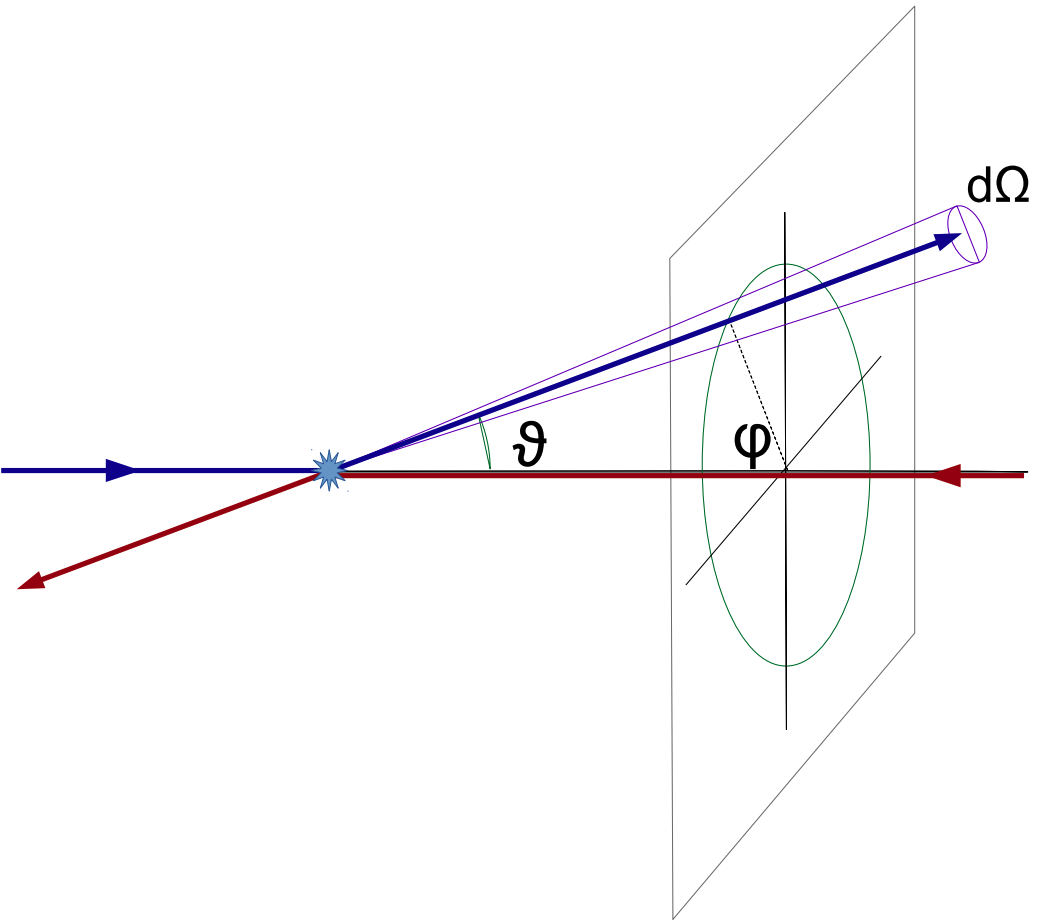
\includegraphics[width=5.5cm]{Chapter2/DifferentialCrossSection}
%\end{wrapfigure} 
%In experiments with a rotational symmetry, such is the case for ATLAS, it is usual to define the differential cross section ($\frac{d\sigma}{d\Omega}$) as the cross section per solid angle. 
%If the differential cross section is integrated over corresponding the angular range, the cross-section for a specific region ($\sigma_{\varphi}$) is obtained:
%\begin{equation}
%	\sigma_{\vartheta} = \int_{0}^{\vartheta} \int_{0}^{2\pi} \frac{d\sigma}{d\Omega} \textrm{sin}(\vartheta)\, d\phi d\vartheta
%\end{equation}
%with $\vartheta \in [0, \pi]$ is the coverage of the scattering angle. 
%\par
%------------------------------------------


It is usual to define the differential cross-section ($\frac{d\sigma}{d\Omega}$) as the cross-section per solid angle. 
If the differential cross-section is integrated over corresponding the angular range, the cross section 
for a specific region ($\sigma_{\varphi}$) is obtained:

\begin{minipage}{0.45\textwidth}
\begin{equation*}
	\sigma_{\vartheta} = \int_{0}^{\vartheta} \int_{0}^{2\pi} \frac{d\sigma}{d\Omega} \textrm{sin}(\vartheta)\, d\phi d\vartheta
\end{equation*}
where $\vartheta \in [0, \pi]$ is the coverage of the scattering angle. 
\end{minipage} \hfill
\begin{minipage}{0.45\textwidth}
 	  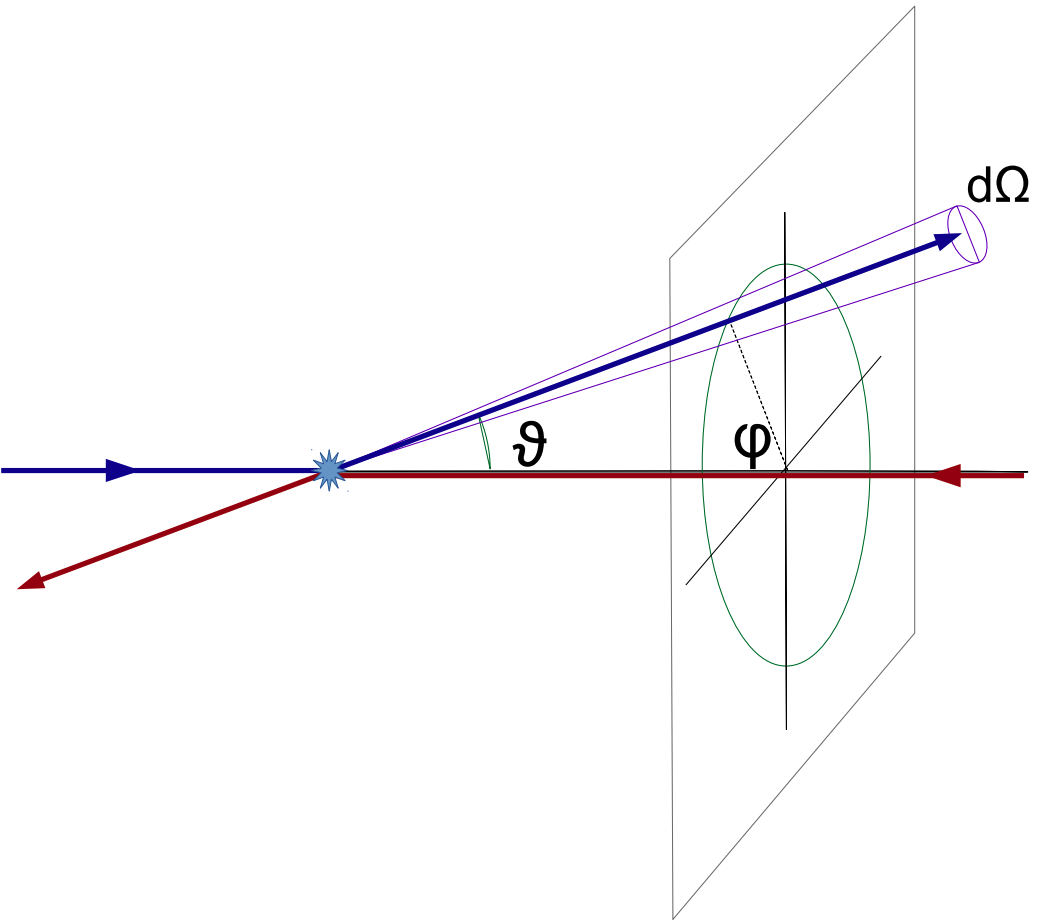
\includegraphics[width = \textwidth]{Chapter2/DifferentialCrossSection}
\end{minipage} 

%\begin{comment}
%\pablo{this paragraph may be removed}
The total cross-section is determined by the amplitude of the scattering matrix $\mathcal{M}$, 
which is independent of the experimental setup. The $\mathcal{M}$, also known as scattering amplitude, 
relates the initial state and the final state of a physical system undergoing a scattering process.
The $\mathcal{M}$ is calculated by summing all possible Feynman diagrams contributing to the hard-scatter
process at the desired order.
Using $\mathcal{M}$, the total cross-section for a process is determined by:
\begin{equation}\label{eq:chap1:Pheno:XS}
	\sigma_{tot} = \int \frac{d\sigma}{d\Omega} \, d\Omega = \int \frac{1}{\Phi} |\mathcal{M}|^{2}\, dQ
\end{equation}
being $\Phi$ the incident particle flux in the process and the parameter $dQ$ describes the kinematic phase space.
%The $\mathcal{M}$ is often referred as Matrix Element (ME).
%\end{comment}
\end{comment}



%POSTAMBLE
\begin{comment}

%\bibliographystyle{../../jhep}
%\bibliography{../../biblio}
asdf
%\end{document}

%ENDPOSTAMBLE
\end{comment}
